\documentclass[11pt,a4paper]{report}

% ===== 核心宏包与中文支持 =====
\usepackage[utf8]{inputenc}
\usepackage{xeCJK}
\usepackage{graphicx}
\usepackage{amsmath, amssymb, amsfonts}
\usepackage{listings}
\usepackage{xcolor}
\usepackage{geometry}
\usepackage{tcolorbox}
\usepackage{booktabs}
\usepackage{tabularx}
\usepackage{setspace}
\usepackage{enumitem}
\usepackage{float}
\usepackage[hidelinks]{hyperref}
\usepackage{bookmark}
\usepackage{fancyhdr}
\usepackage{titlesec}
\usepackage{tocloft}

% 三级标题统一：纯数字编号 + 左对齐（block 模式，CJK 安全）
\titleformat{\chapter}[block]
  {\normalfont\Huge\bfseries\raggedright}
  {\thechapter}{1em}{}
\titlespacing*{\chapter}{0pt}{0pt}{16pt}

\titleformat{\section}[block]
  {\normalfont\Large\bfseries\raggedright}
  {\thesection}{1em}{}
\titlespacing*{\section}{0pt}{14pt}{6pt}

\titleformat{\subsection}[block]
  {\normalfont\large\bfseries\raggedright}
  {\thesubsection}{1em}{}
\titlespacing*{\subsection}{2em}{10pt}{4pt}

% --- PDF 书签与元数据 ---
\hypersetup{
    colorlinks=false,
    pdfborder={0 0 0},
    bookmarks=true,
    bookmarksnumbered=true,
    bookmarksopen=true,
    bookmarksopenlevel=2,
    pdfcreator={XeLaTeX},
    pdftitle={Python BootCamp 完整课程笔记（9章合辑）},
    pdfauthor={黄子扬},
}

% ===== 页面美化设置 =====
\geometry{top=0.7in,bottom=0.8in,left=0.6in,right=0.6in}
\onehalfspacing
\tcbuselibrary{skins,breakable}
\setlength{\parindent}{0pt}
\setlength{\parskip}{0.6em}

% ===== 代码样式配置 =====
\definecolor{mainblue}{RGB}{0,51,102}
\definecolor{examred}{RGB}{180,0,0}
\definecolor{codebg}{RGB}{248,248,248}
\definecolor{commentgreen}{RGB}{0,128,0}

\lstset{
    backgroundcolor=\color{codebg},
    basicstyle=\ttfamily\footnotesize,
    keywordstyle=\color{blue}\bfseries,
    commentstyle=\color{commentgreen},
    stringstyle=\color{orange},
    breaklines=true,
    showstringspaces=false,
    frame=single,
    frameround=tttt,
    framesep=6pt,
    rulecolor=\color{gray!40},
    xleftmargin=0em,
    numbers=left,
    numbersep=5pt,
    numberstyle=\tiny\color{gray},
    language=Python,
    morekeywords={None, True, False, plt, np, pd, fig, ax, subplots, DataFrame, Series, loc, iloc, at, iat, merge, join, groupby, def, return, if, elif, else, for, in, while, break, continue, pass, class, self, super, property, lambda, inplace, astype, cut, assign, import, as, from, with, try, except, raise, and, or, not, del, range, len, type, sum, min, max, sorted},
}

% ===== 自定义教学框 =====
\newtcolorbox{concept}[1]{colback=blue!5, colframe=mainblue, fonttitle=\bfseries, title={{【Concept / 核心概念】#1}}, arc=3pt, breakable}
\newtcolorbox{warning}[1]{colback=red!5, colframe=examred, fonttitle=\bfseries, title={{【Warning / 避坑指南】#1}}, arc=3pt, breakable}
\newtcolorbox{examplebox}[1]{colback=green!2, colframe=green!40!black, fonttitle=\bfseries, title={{【Example / 实战案例】#1}}, arc=2pt, breakable}

% ===== 页眉页脚 =====
\pagestyle{fancy}
\fancyhf{}
\fancyhead[L]{\small\bfseries\leftmark}
\fancyhead[R]{\small\thepage}
\renewcommand{\headrulewidth}{0.5pt}

% ===== 目录美化 =====
\renewcommand{\cftchapleader}{\cftdotfill{\cftdotsep}}
\renewcommand{\cftsecleader}{\cftdotfill{\cftdotsep}}
\setlength{\cftbeforechapskip}{0.4em}
\setlength{\cftbeforesecskip}{0.2em}
\renewcommand{\cftchapfont}{\bfseries\color{mainblue}}
\renewcommand{\cftsecfont}{\color{mainblue!80!black}}
\renewcommand{\cftchappagefont}{\bfseries\color{mainblue}}

% ===== 行内代码着色 =====
\let\oldtexttt\texttt
\renewcommand{\texttt}[1]{\textcolor{mainblue}{\oldtexttt{#1}}}

% ===== 文档信息 =====

\begin{document}

% --- 封面 ---
\begin{titlepage}
\thispagestyle{empty}
\begin{center}

\vspace*{1.5cm}

% 校徽：左 HIT / 右 emlyon
\begin{minipage}[c]{0.48\textwidth}
  \centering
  
\includegraphics[height=2.2cm]{HIT_logo.png}
\end{minipage}
\hfill
\begin{minipage}[c]{0.48\textwidth}
  \centering
  
\includegraphics[height=2.2cm]{emlyon_logo.png}
\end{minipage}

\vspace{1.2cm}

{\large 哈尔滨工业大学 \quad 法国里昂商学院 \\ Harbin Institute of Technology \quad emlyon business school \par}

\vspace{1.2cm}

\rule{\linewidth}{0.5pt}

\vspace{0.8cm}

{\Huge\bfseries Object Oriented Programming \\[0.3em] Python BootCamp \par}

\vspace{0.8cm}

\rule{\linewidth}{0.5pt}

\vspace{1.5cm}

{\Large\textbf{黄子扬} \par}
\vspace{0.3em}
{\large Ziyang Huang \par}
\vspace{0.3em}
{\normalsize 二叉苹果树 \par}

\vfill

{\large \today \par}

\end{center}
\end{titlepage}

% --- 前言 ---
\chapter*{Preface / 前言}
\addcontentsline{toc}{chapter}{Preface / 前言}

本课程 \textbf{Object Oriented Programming}（课程代码 22EM31202C）是哈尔滨工业大学与法国里昂商学院联合举办的\textbf{应用数据科学本科项目（BSc in Applied Data Science）}一年级春季学期专业核心课，共 32 学时、2 学分，考核方式为\textbf{考试课}。课程由 \textbf{Imène BRIGUI} 老师与 \textbf{Saeed VARASTEN YAZDI} 老师联合讲授。

课程从 Python 变量与数据类型起步，逐步深入控制结构、数据结构、模块与包、面向对象编程（类、对象、封装、继承、多态）、文件 IO 与异常处理，最终覆盖数据科学标准库 Matplotlib 和 Pandas 的实战应用，强调理论与实践并重。

\vspace{1em}

\noindent \textbf{关于作者}：黄子扬（ID：二叉苹果树），哈尔滨工业大学经济与管理学院 2025 级大数据管理与应用（中外合作办学）本科生。这份笔记诞生于期末备考阶段——将 9 章课程 PDF 逐一拆解，用 \LaTeX{} 重排为结构化双语笔记，确保覆盖原课件全部内容。初稿完成后，借助 Claude Code + DeepSeek V4 Pro 辅助完成了格式优化、标题统一、附录速查、封面排版等打磨工作，最终形成这份完整课程笔记。

相关资源与更新见 GitHub：\href{https://github.com/huangziyangggg/OOP-Course-Notes}{\texttt{huangziyangggg/OOP-Course-Notes}}

\newpage

\tableofcontents
\newpage

% ============================================================
\chapter{01 - Variables \& Data Types / 变量与数据类型}
% ============================================================



% ======================================================================
\section{Variables / 变量基础}
% ======================================================================

\begin{concept}{What is a Variable? / 什么是变量？}
    In Python, variables are names that can be assigned a value and then used to refer to that value throughout your code. \\
    在 Python 中，变量是可以被赋值并在代码中反复引用的名称。

    Variables are fundamental to programming for two reasons:
    \begin{enumerate}[itemsep=0.3em]
        \item \textbf{Keep values accessible / 保持值可访问}：You can assign the result of a time-consuming operation to a variable so your program doesn't have to perform the operation each time you need the result.
        \item \textbf{Give values context / 赋予值上下文}：The number 28 could mean lots of different things. Giving it a name like \texttt{num\_students} makes the meaning clear.
    \end{enumerate}
\end{concept}

\subsection{The Assignment Operator / 赋值运算符}
\begin{concept}{How it works / 赋值逻辑}
    The \texttt{=} symbol is called the \textbf{assignment operator}. It takes the value on the \textbf{right} and assigns it to the name on the \textbf{left}. \\
    Python 使用 \texttt{=} 符号进行赋值。它将等号右侧的值"绑定"到左侧的名字上。
\end{concept}

\begin{examplebox}{Basic Assignment / 基础赋值}
\begin{lstlisting}
age = 25
print(age)      # Output: 25
\end{lstlisting}
\end{examplebox}

\begin{concept}{How print() Works / print() 的工作原理}
    \texttt{print()} is a function that displays output. Python looks for the variable name, finds its assigned value, and \textbf{replaces} the variable name with its value before calling the function. \\
    \texttt{print()} 是一个函数，用于显示输出。Python 先查找变量名对应的值，\textbf{用值替换}变量名后再调用函数。
\end{concept}

\subsection{Naming Rules \& Conventions / 命名规则与规范}

\begin{itemize}[itemsep=0.3em]
    \item \textbf{Valid Characters / 合法字符}：Uppercase and lowercase letters (A–Z, a–z), digits (0–9), and underscores (\_). Variable names can be as long or as short as you like.
    \item \textbf{Case Sensitivity / 大小写敏感}：\texttt{age} is not the same as \texttt{Age}. Using \texttt{print(Age)} when only \texttt{age} is defined will raise a \texttt{NameError}.
    \item \textbf{Style / 规范}：Common practice is to write variable names in \texttt{lower\_case\_with\_underscores} (e.g., \texttt{car\_length}).
\end{itemize}

\begin{warning}{Variable Name Rules / 变量命名禁忌}
    \begin{itemize}
        \item \textbf{No Digit Start / 严禁数字开头}：Names cannot begin with a digit. \texttt{3text = 4} is invalid.
        \item \textbf{Reserved Words / 保留字}：Do NOT name variables \texttt{print}, \texttt{for}, \texttt{in}, \texttt{list}, \texttt{str}, \texttt{int} — these are built-in functions you will override.
        \item \textbf{Meaningful Names / 命名要有意义}：Always use names that describe the data (e.g., \texttt{car\_length} instead of \texttt{L}).
        \item \textbf{Don't make names too long / 不要太长}：Find a balance between descriptiveness and length.
    \end{itemize}
\end{warning}

\begin{examplebox}{Valid and Invalid Names / 合法与非法命名}
\begin{lstlisting}
# Valid names / 合法命名
test1 = 1
_alpha = 2
L = 3
car_length = 2000

# Invalid names / 非法命名
# 3text = 4         # Error: cannot start with digit
# my-var = 5        # Error: hyphen is not allowed
\end{lstlisting}
\end{examplebox}

\subsection{Comments / 代码注释}

\begin{concept}{What are Comments? / 什么是注释？}
    Comments are lines of text that don't affect how a program runs. They document what code does or why the programmer made certain decisions. \\
    注释是不影响程序运行的文本行，用于记录代码用途或编程决策的原因。

    The most common way to write a comment is to begin a new line with the \texttt{\#} character. When Python runs your code, it ignores lines starting with \texttt{\#}.
\end{concept}

\begin{examplebox}{Comment Examples / 注释示例}
\begin{lstlisting}
# This variable stores the car length in cm
L = 2000
print(L)

H = 146   # This variable stores the car height in cm
print(H)
\end{lstlisting}
\end{examplebox}

% ======================================================================
\section{Data Types / 数据类型百科}
% ======================================================================

\begin{concept}{What is a Data Type? / 什么是数据类型？}
    The term \textbf{data type} refers to what kind of data a value represents. Python has several built-in data types. \\
    \textbf{数据类型}指一个值代表什么类型的数据。Python 有多种内置数据类型。
\end{concept}

\subsection{Primitive Types / 原始类型}

\medskip
\centering
\renewcommand{\arraystretch}{1.5}
\begin{tabular}{@{}llll@{}}
\toprule
\textbf{Type / 类型} & \textbf{Keyword} & \textbf{Description / 描述} & \textbf{Example / 示例} \\ \midrule
Integer / 整数 & \texttt{int} & Whole numbers / 整数 & \texttt{100} \\
Float / 浮点数 & \texttt{float} & Decimal numbers / 小数 & \texttt{10.7} \\
Boolean / 布尔值 & \texttt{bool} & \texttt{True} or \texttt{False} (Capitalized!) & \texttt{True} \\
String / 字符串 & \texttt{str} & Text data / 引号内的文本 & \texttt{"Hello"} \\ \bottomrule
\end{tabular}
\medskip

\subsection{The type() Function / type() 函数}

\begin{concept}{Determining Data Type / 确定数据类型}
    The \texttt{type()} function is used to determine the data type of a given value or variable. \\
    \texttt{type()} 函数用于判断任何值或变量的数据类型。
\end{concept}

\begin{examplebox}{Using type() / type() 实操}
\begin{lstlisting}
num = 100               # An integer variable
length = 10.7           # A floating point variable

print(type(num))        # <class 'int'>
print(type(length))     # <class 'float'>
\end{lstlisting}
\end{examplebox}

\subsection{Boolean Data Type / 布尔类型}

\begin{concept}{True or False / 真与假}
    The boolean data type (\texttt{bool}) can have only one of two values: \texttt{True} or \texttt{False} (both must be \textbf{capitalized}!). \\
    布尔型只有两个值：\texttt{True}（真）和 \texttt{False}（假），首字母\textbf{必须大写}！

    Booleans are fundamental for conditional expressions — we will explore them more in later chapters.
\end{concept}

\begin{examplebox}{Boolean Examples / 布尔值示例}
\begin{lstlisting}
is_finished = True
print(type(is_finished))    # <class 'bool'>

is_finished = False
print(type(is_finished))    # <class 'bool'>
\end{lstlisting}
\end{examplebox}

% ======================================================================
\section{Strings: Complete Guide / 字符串完全指南}
% ======================================================================

\subsection{Properties \& Creation / 属性与创建}

\begin{concept}{Three Key Properties / 三大核心属性}
    Strings in Python are identified as a contiguous set of characters represented in quotation marks. They have three important properties:
    \begin{enumerate}[itemsep=0.3em]
        \item \textbf{Characters / 字符}：Strings contain individual letters or symbols called characters.
        \item \textbf{Length / 长度}：Strings have a length, defined as the number of characters the string contains. Use \texttt{len()} to get it.
        \item \textbf{Sequence / 序列}：Characters in a string appear in a sequence — each character has a \textbf{numbered position} (index) in the string.
    \end{enumerate}
    字符串是引号内的连续字符集。三个核心属性：(1)由字符组成 (2)有长度 (3)字符按序列排列。
\end{concept}

\subsection{Quotes and Escape Characters / 引号与转义字符}

\begin{warning}{Quote Conflicts / 引号冲突}
    If you use double quotes inside a string delimited by double quotes, you'll get an error:
    \begin{lstlisting}
# text1 = "She said, "What time is it?""  # ERROR!
    \end{lstlisting}
    \textbf{Solutions / 解决方案}：
    \begin{enumerate}
        \item Use single quotes outside, double quotes inside:
        \texttt{text1 = 'She said, "What time is it?"'}
        \item Use the escape character \texttt{\textbackslash}:
        \texttt{text1 = "She said, \textbackslash"What time is it?\textbackslash""}
    \end{enumerate}
\end{warning}

\begin{examplebox}{Escape Character / 转义字符示例}
\begin{lstlisting}
text1 = 'She said, "What time is it?"'
text2 = "She said, \"What time is it?\""
print(text1)    # She said, "What time is it?"
print(text2)    # She said, "What time is it?"
\end{lstlisting}
\end{examplebox}

\subsection{Determine the Length of a String / 获取字符串长度}

\begin{examplebox}{Using len() / len() 函数}
    \texttt{len()} is a Python built-in function that returns the number of characters in a string (including spaces).
\begin{lstlisting}
text2 = "This is a test string"
print(len(text2))   # Output: 22
\end{lstlisting}
\end{examplebox}

\subsection{Multiline Strings / 多行字符串}

\begin{concept}{Two Ways to Create Multiline Strings / 两种多行字符串方式}
    To deal with long strings, you can break them up across multiple lines:
    \begin{enumerate}[itemsep=0.3em]
        \item \textbf{Backslash method / 反斜杠法}：Put a backslash (\texttt{\textbackslash}) at the end of each line except the last.
        \item \textbf{Triple quotes method / 三引号法}：Use triple quotes (\texttt{"""} or \texttt{'''}) as delimiters.
    \end{enumerate}
\end{concept}

\begin{examplebox}{Multiline String Examples / 多行字符串示例}
\begin{lstlisting}
# Method 1: Backslash / 反斜杠法
long_text = "This planet has--or rather had--a problem, which was \
this: most of the people living on it were unhappy for pretty much of the time."
print(long_text)

# Method 2: Triple quotes / 三引号法
long_text = """This planet has--or rather had--a problem, which was
this: most of the people living on it were unhappy for pretty much of the time."""
print(long_text)
\end{lstlisting}
\end{examplebox}

\subsection{Concatenation, Indexing, and Slicing / 拼接、索引与切片}

\subsubsection{Concatenation / 字符串拼接}
\begin{concept}{Joining Strings with + / 用 + 拼接字符串}
    You can combine, or concatenate, two strings using the \texttt{+} operator.
\end{concept}

\begin{examplebox}{Concatenation Example / 拼接示例}
\begin{lstlisting}
string1 = "Hello"
string2 = "World"
string3 = string1 + string2
print(string3)      # Output: HelloWorld (no space!)
\end{lstlisting}
\end{examplebox}

\subsubsection{Indexing / 索引}
\begin{concept}{The Rule of 0 / 从 0 开始计数}
    In Python, counting always starts at \textbf{zero (0)}. Each character in a string has a numbered position called an \textbf{index}. \\
    Python 计数永远从 0 开始。字符串中的每个字符都有一个称为索引的编号位置。
\end{concept}

\begin{examplebox}{Positive and Negative Indexing / 正索引与负索引}
\begin{lstlisting}
text = "Python BootCamp"

# Positive index / 正索引（从左到右，从 0 开始）
print(text[0])      # 'P' (第一个字符)
print(text[7])      # 'B'

# Negative index / 负索引（从右到左，从 -1 开始）
print(text[-1])     # 'p' (最后一个字符)
print(text[-5])     # 't'
\end{lstlisting}
\end{examplebox}

\subsubsection{Slicing / 切片}
\begin{concept}{Extracting Substrings / 提取子字符串}
    You can extract a portion of a string (called a \textbf{substring}) by inserting a colon between two index numbers inside square brackets: \texttt{[start:stop]}. \\
    \textbf{Critical Rule / 关键规则}：Inclusive on the left, \textbf{EXCLUSIVE} on the right. \\
    切片格式为 \texttt{[start:stop]}，左闭右开——包含 start，不包含 stop。
\end{concept}

\begin{examplebox}{Slicing Examples / 切片实战}
\begin{lstlisting}
text = "Python BootCamp"

# Basic slicing [start:stop]
print(text[0:6])    # 'Python' (indices 0,1,2,3,4,5 — NOT 6)
print(text[7:11])   # 'Boot'

# Omit start: assumes 0
print(text[:6])     # 'Python' (same as text[0:6])

# Omit stop: goes to the end
print(text[7:])     # 'BootCamp'

# Both omitted: the whole string
print(text[:])      # 'Python BootCamp'
\end{lstlisting}
\end{examplebox}

\subsection{Immutability / 不可变性}

\begin{warning}{Strings Are Immutable / 字符串不可修改}
    You cannot change characters once a string is created. Strings are \textbf{immutable}. \\
    字符串一旦创建就不可修改。试图执行 \texttt{text[6] = '\_'} 会抛出 \texttt{TypeError}：\texttt{'str' object does not support item assignment}.

    \textbf{Solution / 解决方法}：Most string methods return a \textbf{modified copy} — you must reassign to keep the result.
\end{warning}

\begin{examplebox}{Immutability Demonstration / 不可变性演示}
\begin{lstlisting}
name = "Emlyon"
name.upper()            # Returns "EMLYON" but does NOT change 'name'!
print(name)             # Still "Emlyon"

name = name.upper()     # Correct: reassign the result
print(name)             # Now "EMLYON"
\end{lstlisting}
\end{examplebox}

\subsection{String Methods / 字符串方法大全}

\begin{concept}{What are String Methods? / 什么是字符串方法？}
    Strings come bundled with special functions called \textbf{string methods} that you can use to manipulate strings. The dot (\texttt{.}) tells Python that what follows is the name of a method. \\
    字符串附带特殊的函数称为字符串方法，点号 (\texttt{.}) 表示接下来是方法名。
\end{concept}

\begin{examplebox}{Common String Methods / 常用字符串方法}
\begin{lstlisting}
# 1. Case Conversion / 大小写转换
print("Python BootCamp".lower())        # 'python bootcamp'
print("Python BootCamp".upper())        # 'PYTHON BOOTCAMP'

# 2. Removing Whitespace / 去除首尾空白
print(" Python BootCamp".strip())       # 'Python BootCamp'

# 3. Counting Substrings / 统计子串出现次数
text = "Python BootCamp is the best Python program ever!"
print(text.count("Python"))             # Output: 2

# 4. Finding Substring Position / 查找子串位置
print(text.find("Python"))              # Output: 0 (first occurrence)
print(text.find("python"))              # Output: -1 (not found!)

# 5. Check Start and End / 检查首尾
print("Python BootCamp".startswith('P'))  # True
print("Python BootCamp".endswith('p'))    # False

# 6. Replace / 替换
print("Hello World".replace("World", "Python"))  # 'Hello Python'
\end{lstlisting}
\end{examplebox}

\begin{warning}{find() Returns -1 When Not Found / find() 找不到返回 -1}
    The \texttt{find()} method returns the index of the first occurrence, or \textbf{-1} if the substring is not found. This is different from indexing with \texttt{[]}, which would raise an error. \\
    \texttt{find()} 找不到时返回 \texttt{-1}（不是报错），与直接用 \texttt{[]} 索引不同。
\end{warning}

% ======================================================================
\section{The None Data Type / 特殊类型 None}
% ======================================================================

\begin{concept}{NoneType / 空值类型}
    The \texttt{None} keyword is used to define a null value, or no value at all. \\
    \texttt{None} 用于表示"空值"或"无值"。

    \textbf{Critical Distinctions / 关键区分}：
    \begin{itemize}
        \item \texttt{None} is NOT the same as \texttt{0}
        \item \texttt{None} is NOT the same as \texttt{False}
        \item \texttt{None} is NOT the same as an empty string \texttt{""}
        \item \texttt{None} is a data type of its own (\texttt{NoneType})
        \item Only \texttt{None} can be \texttt{None}
    \end{itemize}
\end{concept}

\begin{examplebox}{None Example / None 示例}
\begin{lstlisting}
my_var = None
print(my_var)       # None
print(type(my_var)) # <class 'NoneType'>
\end{lstlisting}
\end{examplebox}

% ======================================================================
\section{Operators / 运算符}
% ======================================================================

\subsection{Arithmetic Operators / 算术运算符}

\medskip
\centering
\renewcommand{\arraystretch}{1.5}
\begin{tabular}{@{}lll@{}}
\toprule
\textbf{Operator} & \textbf{Operation / 操作} & \textbf{Example / 示例} \\ \midrule
\texttt{+}  & Addition / 加法          & \texttt{2 + 2 = 4} \\
\texttt{-}  & Subtraction / 减法       & \texttt{5 - 2 = 3} \\
\texttt{*}  & Multiplication / 乘法    & \texttt{3 * 2 = 6} \\
\texttt{/}  & Division / 标准除法      & \texttt{5 / 2 = 2.5} \\
\texttt{//} & Floor Division / 整除    & \texttt{5 // 2 = 2} \\
\texttt{**} & Exponent / 幂运算        & \texttt{3 ** 2 = 9} \\ \bottomrule
\end{tabular}
\medskip

\begin{warning}{/ vs // 的区别}
    In Python 3, \texttt{/} denotes \textbf{standard division} (always returns float), while \texttt{//} denotes \textbf{floor division} (integer division, discards the remainder). \\
    Python 3 中，\texttt{/} 是标准除法（返回 float），\texttt{//} 是整除（丢弃余数）。
\end{warning}

\begin{examplebox}{Arithmetic Operators Demo / 算术运算符演示}
\begin{lstlisting}
print(2 + 2)        # 4
print(3 * 2)        # 6
print(3 ** 2)       # 9
print(5 / 2)        # 2.5 (standard division)
print(5 // 2)       # 2 (floor division)
\end{lstlisting}
\end{examplebox}

\subsection{Arithmetic on Strings / 字符串上的算术运算}

\begin{concept}{Operators work differently on strings / 运算符对字符串有特殊行为}
    Some arithmetic operators also work on \texttt{str} type:
    \begin{itemize}
        \item \texttt{+} on strings: concatenation / 拼接——将两个字符串首尾相接
        \item \texttt{*} between string and int: repetition / 重复——将字符串重复指定次数
    \end{itemize}
    注意：\texttt{+} 两边是字符串时是拼接（不是算术加法）；\texttt{*} 左边是字符串、右边是整数时是重复。
\end{concept}

\begin{examplebox}{String Arithmetic / 字符串运算}
\begin{lstlisting}
print('2' + '4')        # '24' (concatenation, not addition!)
print(2 * 'S')          # 'SS' (repetition)
# print('2' * '4')      # Error! Cannot multiply string by string
\end{lstlisting}
\end{examplebox}

\subsection{Comparison Operators / 比较运算符}

\begin{concept}{Comparison Produces Boolean / 比较结果总是布尔值}
    The result of a comparison is always a boolean value (\texttt{True} or \texttt{False}). \\
    比较运算的结果永远是布尔值（\texttt{True} 或 \texttt{False}）。
\end{concept}

\medskip
\centering
\renewcommand{\arraystretch}{1.5}
\begin{tabular}{@{}lll@{}}
\toprule
\textbf{Operator} & \textbf{Description / 描述} & \textbf{Example / 示例} \\ \midrule
\texttt{==} & Equal / 等于               & \texttt{1 == 1} $\rightarrow$ \texttt{True} \\
\texttt{!=} & Not equal / 不等于          & \texttt{2.3 != 2.313} $\rightarrow$ \texttt{True} \\
\texttt{<}  & Less than / 小于             & \texttt{2.5 < 9} $\rightarrow$ \texttt{True} \\
\texttt{>}  & Greater than / 大于          & \texttt{2.4 > 2.399} $\rightarrow$ \texttt{True} \\
\texttt{<=} & Less than or equal / 小于等于  & \texttt{3 <= 3} $\rightarrow$ \texttt{True} \\
\texttt{>=} & Greater than or equal / 大于等于 & \texttt{2.4 >= 2.399} $\rightarrow$ \texttt{True} \\ \bottomrule
\end{tabular}
\medskip

\begin{examplebox}{Comparison Examples / 比较运算示例}
\begin{lstlisting}
print(2.5 < 3)          # True
print(2 == 2)           # True
print(2 != 3)           # True
print(5 >= 5)           # True
print(10 < 3)           # False
\end{lstlisting}
\end{examplebox}

\subsection{Logical Operators / 逻辑运算符}

\begin{concept}{Combining Boolean Values / 组合布尔值}
    Logical operators take boolean values as input and produce either \texttt{True} or \texttt{False} as output. \\
    逻辑运算符接收布尔值并返回布尔值。
\end{concept}

\medskip
\centering
\renewcommand{\arraystretch}{1.5}
\begin{tabularx}{\textwidth}{@{}l>{\raggedright\arraybackslash}X>{\raggedright\arraybackslash}X@{}}
\toprule
\textbf{Operator} & \textbf{Description / 描述} & \textbf{Rule / 规则} \\ \midrule
\texttt{x or y}  & If either is True $\rightarrow$ True; otherwise False. / 任一为真则真 & Returns \texttt{True} if at least one is \texttt{True} \\
\texttt{x and y} & If both are True $\rightarrow$ True; otherwise False. / 两者为真才真 & Returns \texttt{True} only if \textbf{both} are \texttt{True} \\
\texttt{not x}   & Reverses the boolean value. / 取反 & Returns \texttt{False} if \texttt{x} is \texttt{True}; \texttt{True} if \texttt{x} is \texttt{False} \\ \bottomrule
\end{tabularx}
\medskip

\begin{examplebox}{Logical Operators Demo / 逻辑运算符演示}
\begin{lstlisting}
# or: True if either is True
print((2 == 3) or (4 < 5))      # True (4 < 5 is True)

# and: True only if BOTH are True
print((2 == 3) and (4 < 5))     # False (2 == 3 is False)

# not: Reverses the boolean
print(not (2 == 3))             # True (reverses False to True)
print(not True)                 # False
\end{lstlisting}
\end{examplebox}

% ======================================================================
\section{Type Casting / 类型转换}
% ======================================================================

\begin{concept}{Converting Between Types / 类型之间的转换}
    If you want to change one data type to another, use the following functions: \\
    使用以下函数进行类型转换：\texttt{int()}, \texttt{str()}, \texttt{float()}, \texttt{bool()}.

    These four data types (\texttt{int}, \texttt{float}, \texttt{str}, \texttt{bool}) are called \textbf{Primitive Types}.
\end{concept}

\begin{examplebox}{Type Casting Examples / 类型转换示例}
\begin{lstlisting}
print(int(9.9))         # 9 (truncates, does NOT round!)
print(str(5))           # '5'
print(bool(1))          # True
# print(int("Yes!"))    # ValueError: invalid literal for int()
\end{lstlisting}
\end{examplebox}

\begin{warning}{String + Int = Error! / 字符串 + 整数 = 报错！}
    You MUST cast \texttt{str} to \texttt{int} before doing arithmetic operations:
\begin{lstlisting}
# Wrong / 错误
a = 34
b = "10"
# print(a + b)        # TypeError! Cannot add int and str

# Correct / 正确
a = 34
b = "10"
print(a + int(b))       # 44
\end{lstlisting}
\end{warning}

\begin{concept}{Truthiness / 真值判定规则}
    Almost any value is evaluated to \texttt{True} if it has some sort of content:
    \begin{itemize}[itemsep=0.3em]
        \item Any string is \texttt{True}, \textbf{except} empty strings (\texttt{""}). / 任何非空字符串为 \texttt{True}。
        \item Any number is \texttt{True}, \textbf{except} \texttt{0}. / 任何非零数字为 \texttt{True}。
        \item \texttt{bool(0)} $\rightarrow$ \texttt{False}; \texttt{bool("")} $\rightarrow$ \texttt{False}
    \end{itemize}
    \textbf{Falsy values / 假值（以下值会被判为 False）}：\texttt{0}, \texttt{0.0}, \texttt{""}, \texttt{None}, \texttt{False}, empty containers / 空容器.
\end{concept}

% ======================================================================
\section{String Formatting / 字符串格式化输出（四种方法）}
% ======================================================================

\begin{concept}{The Goal / 目标}
    Suppose you have \texttt{name = "Doctor Strange"}, \texttt{heads = 2}, \texttt{arms = 3}. \\
    You want to display: \textbf{"Doctor Strange has 2 heads and 3 arms."}

    There are \textbf{four} ways to achieve this in Python.
\end{concept}

\subsection{Method 1: Commas in print() / 用逗号分隔}

\begin{examplebox}{Comma Method / 逗号法}
\begin{lstlisting}
name = "Doctor Strange"
heads = 2
arms = 3
print(name, "has", str(heads), "heads and", str(arms), "arms.")
# Output: Doctor Strange has 2 heads and 3 arms.
\end{lstlisting}
    Note: \texttt{print()} automatically inserts spaces between comma-separated items. You must convert numbers to strings with \texttt{str()}. \\
    注意：\texttt{print()} 会自动在逗号分隔的项之间插入空格。数字必须用 \texttt{str()} 转为字符串。
\end{examplebox}

\subsection{Method 2: Concatenation with + / 字符串拼接法}

\begin{examplebox}{Concatenation Method / 拼接法}
\begin{lstlisting}
print(name + " has " + str(heads) + " heads and " + str(arms) + " arms.")
# Output: Doctor Strange has 2 heads and 3 arms.
\end{lstlisting}
    Note: Tedious! Must manually add spaces and convert numbers to strings. \\
    注意：这种方法写起来很繁琐！必须手动添加空格、用 \texttt{str()} 转换数字。
\end{examplebox}

\subsection{Method 3: f-strings (Best Practice, Python 3.6+) / f-字符串（推荐）}

\begin{concept}{f-strings / f-字符串格式化}
    Two important things to notice:
    \begin{enumerate}
        \item The string literal starts with the letter \texttt{f} before the opening quotation mark.
        \item Variable names surrounded by curly braces \texttt{\{} and \texttt{\}} are replaced with their corresponding values \textbf{without} needing \texttt{str()}.
    \end{enumerate}
    f-strings are only available in \textbf{Python version 3.6 and above}.
\end{concept}

\begin{examplebox}{f-string Example / f-字符串示例}
\begin{lstlisting}
print(f"{name} has {heads} heads and {arms} arms.")
# Output: Doctor Strange has 2 heads and 3 arms.
\end{lstlisting}
\end{examplebox}

\subsection{Method 4: .format() Method / .format() 方法}

\begin{examplebox}{.format() Method / .format() 方法示例}
\begin{lstlisting}
print("{} has {} heads and {} arms.".format(name, heads, arms))
# Output: Doctor Strange has 2 heads and 3 arms.
\end{lstlisting}
    Curly braces \texttt{\{\}} act as placeholders, filled by \texttt{.format()} arguments in order.
\end{examplebox}

\subsection{Method 5 (Legacy): \% Operator / \% 运算符（旧式）}

\begin{examplebox}{\% Operator / \% 运算符示例}
\begin{lstlisting}
print("%s has %s heads and %s arms." % (name, heads, arms))
# Output: Doctor Strange has 2 heads and 3 arms.
\end{lstlisting}
    \texttt{\%s} is a placeholder for string; values are provided in parentheses after \texttt{\%}.
\end{examplebox}

% ======================================================================
\section{User Input / 用户输入}
% ======================================================================

\begin{concept}{The input() Function / input() 函数}
    The \texttt{input()} function gets input from the user. It:
    \begin{itemize}[itemsep=0.3em]
        \item Displays a \textbf{prompt} (a string that tells the user what to enter).
        \item Waits for the user to type something and press Enter.
        \item \textbf{Always returns a string} — even if the user types a number!
    \end{itemize}
\end{concept}

\begin{examplebox}{input() Examples / 用户输入示例}
\begin{lstlisting}
# Basic usage
name = input()
print(name)

# With a prompt / 带提示信息的输入
age = input("Please enter your age: ")
print(age)              # age is a STRING, not a number!
print(type(age))        # <class 'str'>

# Convert to number if needed / 如需数字，必须转换
age = int(input("Please enter your age: "))
print(age + 1)          # Now it works as a number
\end{lstlisting}
\end{examplebox}

\begin{warning}{input() Always Returns a String / input() 永远返回字符串}
    Even if the user types \texttt{42}, the result is the string \texttt{"42"}, NOT the integer \texttt{42}. Use \texttt{int()} or \texttt{float()} to convert. \\
    即使用户输入 42，返回的也是字符串 \texttt{"42"}，需要用 \texttt{int()} 或 \texttt{float()} 转换后才能做数学运算。
\end{warning}

% ======================================================================
\section{Quick Reference / 速查表}
% ======================================================================

\medskip
\centering
\small
\renewcommand{\arraystretch}{1.3}
\begin{tabular}{@{}ll@{}}
\toprule
\textbf{Operation / 操作} & \textbf{Syntax / 语法} \\ \midrule
赋值 & \texttt{x = 10} \\
检查类型 & \texttt{type(x)} \\
获取长度 & \texttt{len(s)} \\
索引（正） & \texttt{s[0]} \\
索引（负） & \texttt{s[-1]} \\
切片 & \texttt{s[start:stop]} \\
小写 & \texttt{s.lower()} \\
大写 & \texttt{s.upper()} \\
去空白 & \texttt{s.strip()} \\
计数 & \texttt{s.count(sub)} \\
查找 & \texttt{s.find(sub)} \\
开头判断 & \texttt{s.startswith(prefix)} \\
结尾判断 & \texttt{s.endswith(suffix)} \\
替换 & \texttt{s.replace(old, new)} \\
转整数 & \texttt{int(x)} \\
转浮点 & \texttt{float(x)} \\
转字符串 & \texttt{str(x)} \\
转布尔 & \texttt{bool(x)} \\
f-字符串 & \texttt{f"\{var\}"} \\
用户输入 & \texttt{input(prompt)} \\
整除 & \texttt{//} \\
幂运算 & \texttt{**} \\
逻辑与 & \texttt{and} \\
逻辑或 & \texttt{or} \\
逻辑非 & \texttt{not} \\
等于 & \texttt{==} \\
不等于 & \texttt{!=} \\ \bottomrule
\end{tabular}
\medskip



% ============================================================
\chapter{02 - Control Structures / 控制结构}
% ============================================================



% ======================================================================
\section{Boolean Recap / 布尔值回顾}
% ======================================================================

\begin{concept}{Review from Lecture 01}
    Booleans are one of the data types. They can only be one of two values: \texttt{True} or \texttt{False}. \\
    布尔型只有两个值：\texttt{True}（真）和 \texttt{False}（假）。

    Booleans can result from:
    \begin{itemize}[itemsep=0.3em]
        \item \textbf{Comparison operators}: \texttt{==, !=, <, >, <=, >=} (e.g., \texttt{41 > 42} $\rightarrow$ \texttt{False}).
        \item \textbf{Logical operators}: \texttt{and}, \texttt{or}, \texttt{not} — these act on Booleans and produce Booleans.
    \end{itemize}
    布尔值可以通过比较运算符和逻辑运算符产生。这是条件判断的基础。
\end{concept}

% ======================================================================
\section{Conditionals: If-Statements / 条件判断}
% ======================================================================

\subsection{Basic Logic / 基础逻辑}

\begin{concept}{What is an If-Statement? / 什么是 If 语句？}
    If-statements allow you to execute parts of your code based on whether a condition is met. \\
    If 语句允许程序根据条件是否满足来决定执行哪段代码。

    \textbf{The Rule / 核心规则}：As long as the statement after the \texttt{if} keyword evaluates to \texttt{True}, the \textbf{indented} code block will run. If the statement is \texttt{False}, all the indented parts will be skipped. \\
    只要 \texttt{if} 后面的条件为 \texttt{True}，缩进的代码块就会运行。如果为 \texttt{False}，缩进部分会被完全跳过。
\end{concept}

\subsection{The Full Structure: if / elif / else}

\begin{concept}{Three Keywords / 三个关键字}
    \begin{itemize}[itemsep=0.5em]
        \item \textbf{\texttt{if}}：The first condition to check. / 第一个必检条件。
        \item \textbf{\texttt{elif}} (else if)：Checks additional conditions \textbf{only if} the previous \texttt{if} (or \texttt{elif}) was \texttt{False}. / 仅在前面的条件为 \texttt{False} 时才检查额外条件。
        \item \textbf{\texttt{else}}：Runs if \textbf{none} of the above conditions were \texttt{True}. It is the fallback. / 以上所有条件都不满足时的兜底执行。
    \end{itemize}
\end{concept}

\begin{examplebox}{Price Classification / 价格分级案例}
    课件中通过以下案例展示了完整的 \texttt{if-elif-else} 结构：
\begin{lstlisting}
price = 42
if price > 100:
    print("expensive")          # Runs if price > 100
elif price > 50:                # Checked ONLY if price <= 100
    print("moderate")           # Runs if 50 < price <= 100
else:                           # Runs if all above are False
    print("cheap")              # Runs if price <= 50
# Output: cheap
\end{lstlisting}
\end{examplebox}

\begin{warning}{Execution Order / 执行顺序（重要）}
    In an \texttt{if-elif-else} chain:
    \begin{enumerate}[itemsep=0.3em]
        \item Python checks each condition \textbf{from top to bottom}.
        \item The \textbf{first} condition that is \texttt{True} gets executed.
        \item All subsequent conditions are \textbf{skipped} — even if they would also be \texttt{True}!
    \end{enumerate}
    从上到下检查，第一个为真的条件被执行，其余全部跳过！
\end{warning}

\subsection{Inline Conditionals / 行内条件判断}

\begin{examplebox}{Simple If-Statement / 简单 If 判断}
    课件展示了只需判断单个条件的场景：
\begin{lstlisting}
name = "John"
if len(name) < 3:
    print("your name is short!")    # Won't run because len("John") = 4
\end{lstlisting}
    如果条件为 \texttt{False}，缩进代码块什么都不执行。
\end{examplebox}

\begin{concept}{Ternary Operator (One-line if/else) / 三元运算符}
    Python also supports a one-line conditional expression for simple true/false assignments:
\begin{lstlisting}
# Syntax: value_if_true if condition else value_if_false
result = "short" if len(name) < 3 else "not short"
\end{lstlisting}
    三元运算符适合简单的二选一赋值，不适合复杂逻辑。
\end{concept}

% ======================================================================
\section{Functions / 函数基础}
% ======================================================================

\subsection{Why Functions? / 为什么需要函数？}

\begin{concept}{Building Blocks of Python / Python 的积木块}
    Functions are the building blocks of almost every Python program. They're where the real action takes place. \\
    函数是几乎所有 Python 程序的基本构建块，真正的逻辑都在函数里。

    Functions break code into smaller chunks, and are great for:
    \begin{itemize}[itemsep=0.3em]
        \item Tasks that a program uses \textbf{repeatedly} — instead of writing the same code each time, just call the function. \\
        重复使用的任务——不必每次重写相同代码，直接调用函数即可。
        \item Breaking complex problems into manageable pieces. \\
        把复杂问题拆解为可管理的小块。
        \item Making code more readable and maintainable. \\
        让代码更易读、更易维护。
    \end{itemize}
\end{concept}

\begin{concept}{Built-in vs. User-Defined / 内置函数 vs 自定义函数}
    \begin{itemize}[itemsep=0.3em]
        \item \textbf{Built-in functions}：Come built into Python itself (e.g., \texttt{print()}, \texttt{len()}, \texttt{type()}).
        \item \textbf{User-defined functions}：Functions you create yourself to perform specific tasks.
    \end{itemize}
    你已经用过 \texttt{print()} 和 \texttt{len()} 等内置函数，现在你将学会定义自己的函数。
\end{concept}

\subsection{How Function Calls Work / 函数调用的三步流程}

\begin{concept}{The Three Steps of a Function Call / 函数调用的三个步骤}
    \begin{enumerate}[itemsep=0.5em]
        \item \textbf{Call / 调用}：The function is called, and any arguments are passed to the function as input.
        \item \textbf{Execute / 执行}：The function executes, and some action is performed with the arguments.
        \item \textbf{Return / 返回}：The function returns, and the original function call is \textbf{replaced with the return value}.
    \end{enumerate}
\end{concept}

\begin{examplebox}{Understanding len() / 理解 len() 的执行过程}
\begin{lstlisting}
num_letters = len("emlyon")
print(num_letters)          # Output: 6
\end{lstlisting}
    What happens behind the scenes:
    \begin{enumerate}
        \item \texttt{len()} is called with the argument \texttt{"emlyon"}.
        \item The length of the string is calculated — the number 6.
        \item \texttt{len()} returns 6 and replaces the function call with the value.
        \item Python then assigns \texttt{6} to \texttt{num\_letters}. Equivalent to: \texttt{num\_letters = 6}
    \end{enumerate}
\end{examplebox}

\begin{warning}{Calling Errors / 调用错误}
    Functions like \texttt{len()} require exactly one argument. Calling \texttt{len()} without input will raise a \texttt{TypeError}:\\
    \texttt{TypeError: len() takes exactly one argument (0 given)}

    \begin{itemize}[itemsep=0.3em]
        \item Some functions can be called with \textbf{no} arguments.
        \item Some functions can take \textbf{as many arguments as you like}.
        \item \texttt{len()} requires \textbf{exactly one} argument.
    \end{itemize}
\end{warning}

\subsection{Writing Your Own Functions / 定义自己的函数}

\begin{concept}{Two Parts of a Function / 函数的两大部分}
    Every function has two parts:
    \begin{enumerate}
        \item \textbf{Function Signature / 函数签名}：Defines the name of the function and any inputs (parameters) it expects. Starts with the \texttt{def} keyword.
        \item \textbf{Function Body / 函数体}：Contains the code that runs every time the function is used. Must be \textbf{indented}!
    \end{enumerate}
\end{concept}

\begin{examplebox}{Creating Your First Function / 创建你的第一个函数}
\begin{lstlisting}
def multiply(x, y):         # Function signature: name + parameters
    product = x * y         # Function body (indented!)
    return product          # Return statement: sends result back

# Calling the function
result = multiply(2, 4)     # result = 8
print(result)               # 8
\end{lstlisting}
\end{examplebox}

\begin{concept}{Key Points About User-Defined Functions / 自定义函数要点}
    \begin{itemize}[itemsep=0.3em]
        \item \texttt{def} keyword creates a new function. The function is assigned to a variable with the same name as the function name.
        \item Function names become variables, so they must follow the \textbf{same naming rules} as variables.
        \item You call a user-defined function just like any other function: \texttt{function\_name(arguments)}.
        \item \texttt{return} sends a value back. If there is no \texttt{return} statement, the function returns \texttt{None}.
    \end{itemize}
\end{concept}

\subsection{Arguments and Return Values / 参数与返回值}

\begin{concept}{Key Terminology / 关键术语}
    \begin{itemize}[itemsep=0.5em]
        \item \textbf{Parameter / 形参}：A variable in the function signature that defines what input the function expects (e.g., \texttt{x} and \texttt{y} in \texttt{def multiply(x, y)}).
        \item \textbf{Argument / 实参}：The actual value passed to the function when calling it (e.g., \texttt{2} and \texttt{4} in \texttt{multiply(2, 4)}).
        \item \textbf{Return Value / 返回值}：When a function is done executing, it returns a value as output. The function call is replaced by this value.
    \end{itemize}
\end{concept}

% ======================================================================
\section{Scope / 作用域的秘密}
% ======================================================================

\begin{concept}{Local vs. Global / 局部与全局}
    Names (variable names) are unique. Each function has its own \textbf{local scope} with its own set of names. Code outside functions is in the \textbf{global scope}. \\
    变量名是唯一的。函数内部拥有独立的"局部作用域"，函数外部的代码属于"全局作用域"。
\end{concept}

\begin{examplebox}{Scope Demonstration / 作用域演示}
\begin{lstlisting}
x = 2                       # Global x / 全局变量

def func():
    x = 3                   # NEW local x — does NOT change global x!
    print("Inside:", x)     # Prints 3 (local x)

func()                      # Output: Inside: 3
print("Outside:", x)        # Output: 2 (global x unchanged!)
\end{lstlisting}
    \textbf{关键理解}：函数内部的 \texttt{x = 3} 创建了一个\textbf{全新的局部变量}，不会影响全局的 \texttt{x}。
\end{examplebox}

\begin{concept}{Scope Hierarchy / 作用域层级}
    Scopes have a hierarchy. When Python encounters a variable name:
    \begin{enumerate}[itemsep=0.3em]
        \item First, it looks in the \textbf{local scope} (inside the current function).
        \item If not found, it moves up to the \textbf{global scope} (outside all functions).
        \item If still not found, it raises a \texttt{NameError}.
    \end{enumerate}
    Python 查找变量时先从局部找，找不到才去全局找。
\end{concept}

\begin{examplebox}{Scope Lookup Example / 作用域查找示例}
\begin{lstlisting}
x = 5                       # Global

def func():
    y = x + 5               # x not found locally → uses global x (5)
    print("Inside, y =", y) # Output: Inside, y = 10

func()
print("Outside, x =", x)    # Output: Outside, x = 5
# print(y)                  # NameError! y only exists in func()'s local scope
\end{lstlisting}
    \textbf{注意}：函数内部可以\textbf{读取}全局变量，但不能直接修改它（除非用 \texttt{global} 关键字）。
\end{examplebox}

% ======================================================================
\section{Loops / 循环：程序如何做重复工作}
% ======================================================================

\begin{concept}{Why Loops? / 为什么需要循环？}
    Programmers don't want to work hard — they want to work \textbf{smart}. Loops are the tool for that. \\
    程序员不想做重复劳动——循环就是用来解决这个问题的。

    Imagine your boss wants you to print numbers from 1 to 10. Without loops, you'd write \texttt{print()} ten times. With loops, it's just a few lines. \\
    想象老板让你打印 1 到 10。没有循环你得写 10 次 \texttt{print()}，有了循环只需要几行代码。

    Loops help with tasks that are similar and repetitive, from simple (printing numbers) to complex (nested loops with conditionals).
\end{concept}

\subsection{For Loops / For 循环}

\begin{concept}{For Loop Structure / For 循环结构}
    \begin{lstlisting}
for [every_element] in [my_sequence]:
    do something
    \end{lstlisting}
    \begin{itemize}[itemsep=0.3em]
        \item \texttt{every\_element / 迭代变量}：A variable created by the loop that takes on each value in the sequence, one at a time. / 循环每次迭代时被赋值为序列中的下一个元素。
        \item \texttt{my\_sequence / 被遍历序列}：The sequence to iterate over (list, tuple, string, range, etc.). / 被遍历的序列（列表、元组、字符串、range 等）。
        \item The loop runs once for each item in the sequence. / 循环对序列中的每个元素执行一次。
    \end{itemize}
\end{concept}

\subsubsection{The range() Function / range() 函数}

\begin{concept}{range(start, stop) / range() 详解}
    \texttt{range(1, 11)} produces numbers from \texttt{1} up to (but \textbf{NOT} including) \texttt{11} — i.e., 1, 2, 3, …, 10. \\
    \texttt{range(1, 11)} 产生 1 到 10 的序列，\textbf{不包含}终点 11——和切片一样遵循"左闭右开"规则。

    \textbf{Syntax / 三种语法}：
    \begin{itemize}[itemsep=0.3em]
        \item \texttt{range(stop)} — starts at 0, goes up to (but not including) stop. / 从 0 开始，到 stop-1 结束。
        \item \texttt{range(start, stop)} — starts at start, goes up to (but not including) stop. / 从 start 开始，到 stop-1 结束。
        \item \texttt{range(start, stop, step)} — starts at start, increments by step each time. / 从 start 开始，每次增加 step（步长）。
    \end{itemize}
\end{concept}

\begin{examplebox}{Printing Numbers with for / 用 for 循环打印数字}
\begin{lstlisting}
for i in range(1, 11):
    print(i)                # Prints 1, 2, 3, ..., 10 (each on new line)
\end{lstlisting}
    其中 \texttt{i} 是迭代变量，依次取值为 1, 2, 3, …, 10。
\end{examplebox}

\subsection{While Loops / While 循环}

\begin{concept}{When to Use While? / 什么时候用 While？}
    Used when we only know \textbf{when to stop}, but not \textbf{how many times} to run. \\
    用于只知道"什么时候停"，但不知道要运行几次的情况。

    \textbf{Structure / 结构}：
    \begin{lstlisting}
while [condition]:
    do whatever
    \end{lstlisting}
    Before starting each iteration, the condition is checked. If \texttt{True}, the loop runs. If \texttt{False}, the loop exits.
\end{concept}

\begin{examplebox}{While Loop vs For Loop / While 循环与 For 循环对比}
\begin{lstlisting}
# For loop version — finite, known iterations
for i in range(1, 11):
    print(i)

# While loop version — same result, different approach
counter = 1
while counter < 11:
    print(counter)
    counter = counter + 1       # MUST update counter!
\end{lstlisting}
\end{examplebox}

\begin{warning}{Infinite Loops / 无限循环风险}
    A \texttt{while} loop could run \textbf{forever} if the condition never becomes \texttt{False}! \\
    如果条件永远不为假，\texttt{while} 循环会无休止运行！

    \textbf{Key Differences / For 与 While 的主要区别}：
    \begin{itemize}[itemsep=0.3em]
        \item \textbf{For loop / For 循环}：Creates a variable to iterate over a given sequence. It is \textbf{finite} — you know exactly how many times it will run. / 自动创建迭代变量，遍历已知序列——你确切知道循环会执行多少次。
        \item \textbf{While loop / While 循环}：Does NOT create an iteration variable for you. You must create and update your own counter. It \textbf{could run forever} if you're not careful. / 不会自动创建迭代变量，你必须手动初始化并更新计数器——稍有不慎就会无限循环。
    \end{itemize}
\end{warning}

\subsection{Control Keywords / 循环控制关键字}

\begin{concept}{break, continue, pass / 三大控制关键字}
    这三个关键字可以改变循环的正常执行流程。
\end{concept}

\begin{examplebox}{Control Keywords Demo / 控制关键字对比}
\begin{lstlisting}
# Example: break — 立即终止整个循环
for i in range(1, 11):
    if i == 5:
        break           # Exit loop completely when i = 5
    print(i)            # Prints: 1, 2, 3, 4 (stops at 5)
\end{lstlisting}

\begin{lstlisting}
# Example: continue — 跳过本次循环剩余部分
for i in range(1, 11):
    if i == 5:
        continue        # Skip the rest of THIS iteration
    print(i)            # Prints: 1, 2, 3, 4, 6, 7, 8, 9, 10 (no 5!)
\end{lstlisting}

\begin{lstlisting}
# Example: pass — 占位符，什么都不做
for i in range(1, 11):
    if i == 5:
        pass            # Do nothing — just a placeholder
    print(i)            # Prints: 1, 2, 3, 4, 5, 6, 7, 8, 9, 10
\end{lstlisting}
\end{examplebox}

\medskip
\centering
\renewcommand{\arraystretch}{1.5}
\begin{tabular}{@{}lll@{}}
\toprule
\textbf{Keyword} & \textbf{Effect / 作用} & \textbf{Use Case / 使用场景} \\ \midrule
\texttt{break}    & Aborts the loop entirely / 直接终止整个循环 & 搜索到目标后退出 \\
\texttt{continue} & Skips the rest of the current iteration / 跳过本次循环剩余部分 & 跳过不需要处理的特殊情况 \\
\texttt{pass}     & A placeholder that does nothing / 占位符 & 预留代码位置，防止空代码块报错 \\ \bottomrule
\end{tabular}
\medskip

% ======================================================================
\section{Summary / 速查表}
% ======================================================================

\medskip
\centering
\small
\renewcommand{\arraystretch}{1.3}
\begin{tabular}{@{}ll@{}}
\toprule
\textbf{Structure / 结构} & \textbf{Syntax / 语法} \\ \midrule
If 判断 & \texttt{if condition:} \\
Elif 判断 & \texttt{elif condition:} \\
Else 兜底 & \texttt{else:} \\
定义函数 & \texttt{def name(params):} \\
返回结果 & \texttt{return value} \\
For 循环 & \texttt{for var in sequence:} \\
While 循环 & \texttt{while condition:} \\
终止循环 & \texttt{break} \\
跳过本次 & \texttt{continue} \\
占位符 & \texttt{pass} \\
Range 序列 & \texttt{range(start, stop, step)} \\ \bottomrule
\end{tabular}
\medskip



% ============================================================
\chapter{03 - Data Structures / 数据结构}
% ============================================================



% ======================================================================
\section{Introduction / 什么是数据结构}
% ======================================================================

\begin{concept}{Data Structure / 数据结构}
    A data structure models a collection of data, such as a list of numbers, a row in a spreadsheet, or a record in a database. \\
    数据结构是对数据集合的建模。

    So far, you have been working with fundamental data types like \texttt{str}, \texttt{int}, and \texttt{float}. Many real-world problems are easier to solve when simple data types are combined into more complex data structures. \\
    Python has three built-in data structures that are the focus of this chapter: \textbf{Tuples}, \textbf{Lists}, and \textbf{Dictionaries}. (Plus \textbf{Sets} as a bonus.)
\end{concept}

\subsection{Recap: print() Advanced / print() 进阶参数}

\begin{concept}{sep and end Parameters / sep 和 end 参数}
    \texttt{print()} can print one or multiple objects. By default:
    \begin{itemize}
        \item Objects are separated by a whitespace (\texttt{sep=" "}).
        \item Output ends with a line break (\texttt{end="\textbackslash n"}).
    \end{itemize}
    These behaviors can be changed via the \texttt{sep} and \texttt{end} parameters.
\end{concept}

\begin{examplebox}{print() with sep and end / print() 的 sep 和 end 参数}
\begin{lstlisting}
# Default behavior
print("hello", "there")
# Output: hello there (separated by space, ends with newline)

# Custom sep and end
print("hello", "there", sep="", end="!")
# Output: hellothere! (no separator, ends with "!" instead of newline)
\end{lstlisting}
\end{examplebox}

% ======================================================================
\section{Tuples / 元组 (Parentheses: \texttt{()})}
% ======================================================================

\subsection{What is a Tuple? / 什么是元组？}

\begin{concept}{Sequence Type / 序列类型}
    A \textbf{sequence} is an ordered list of values. Each element in a sequence is assigned an integer, called an \textbf{index}, that determines the order in which the values appear. Just like strings, the index of the first value in a sequence is \texttt{0}. \\
    序列是有序的值列表。每个元素都有一个整数索引，从 0 开始。

    \textbf{Tuples are ordered} because their elements appear in a fixed order. The first element of \texttt{(1, 2, 3)} is 1, the second is 2, the third is 3.
\end{concept}

\subsection{Core Properties / 核心属性}

\begin{itemize}[itemsep=0.5em]
    \item \textbf{Ordered / 有序}：Elements appear in a fixed sequence.
    \item \textbf{Heterogeneous / 异构}：Can contain different types (e.g., \texttt{(1, "John", "Red")}).
    \item \textbf{Index starts at 0}：索引从 0 开始。
    \item \textbf{Immutable / 不可变}：Once created, you cannot change, add, or remove elements.
\end{itemize}

\begin{examplebox}{Tuple Basics / 元组基础}
\begin{lstlisting}
tuple1 = (1, 2, 3)
print(type(tuple1))             # <class 'tuple'>

# Heterogeneous / 异构：可以包含不同类型
tuple2 = (1, "John", "Red")
print(tuple2)                   # (1, 'John', 'Red')

# Empty tuple / 空元组
tuple3 = ()
print(len(tuple3))              # 0
\end{lstlisting}
\end{examplebox}

\subsection{Tuple Operations / 元组操作}

\begin{examplebox}{Length, Indexing, Slicing / 长度、索引、切片}
\begin{lstlisting}
tuple2 = (1, "John", "Red")

# Length / 长度
print(len(tuple2))              # 3

# Indexing / 索引（和字符串一样！）
print(tuple2[1])                # 'John'

# Slicing / 切片
print(tuple2[1:3])              # ('John', 'Red')
\end{lstlisting}
\end{examplebox}

\subsection{Checking Existence / 成员检查}

\begin{examplebox}{The in Keyword / in 关键字}
\begin{lstlisting}
tuple2 = (1, "John", "Red")

if "Red" in tuple2:
    print('There is red')       # This runs
else:
    print('There is no red')
\end{lstlisting}
\end{examplebox}

\subsection{Iteration / 元组遍历}

\begin{examplebox}{Tuples Are Iterable / 元组可迭代}
\begin{lstlisting}
tuple2 = (1, "John", "Red")
for item in tuple2:
    print(item)
# Output:
# 1
# John
# Red
\end{lstlisting}
\end{examplebox}

\begin{warning}{Immutability / 不可变性的后果}
    Like strings, tuples are \textbf{immutable}. You cannot change the value of an element once created. \\
    元组一旦创建就无法修改。试图执行 \texttt{tuple2[1] = "David"} 会抛出 \texttt{TypeError}: \texttt{'tuple' object does not support item assignment}.
\end{warning}

% ======================================================================
\section{Lists / 列表 (Square Brackets: \texttt{[]})}
% ======================================================================

\subsection{What is a List? / 什么是列表？}

\begin{concept}{Another Sequence Type / 另一个序列类型}
    The list data structure is another sequence type in Python. Just like strings and tuples, lists contain items that are indexed by integers, starting with 0.

    A list literal looks almost exactly like a tuple literal, except it uses \textbf{square brackets} \texttt{[ ]} instead of parentheses.
\end{concept}

\begin{examplebox}{Creating Lists / 创建列表}
\begin{lstlisting}
mylist1 = [1, 2, 3]
print(type(mylist1))            # <class 'list'>

# Like tuples, lists can contain different types
mylist2 = [1, "John", "Red"]
print(mylist2)                  # [1, 'John', 'Red']

# Create a list from string using split()
groceries = "eggs, milk, cheese"
grocery_list = groceries.split(", ")
print(grocery_list)             # ['eggs', 'milk', 'cheese']
\end{lstlisting}
\end{examplebox}

\subsection{Mutability / 可变性（关键区别）}

\begin{concept}{Lists Are Mutable / 列表是可变的}
    Unlike tuples, lists are \textbf{mutable}. You can change the value at an index even after the list has been created. \\
    列表是\textbf{可变}的，你可以随时修改、添加或删除其中的元素。
\end{concept}

\begin{examplebox}{Mutability Demo / 可变性演示}
\begin{lstlisting}
grocery_list = ['eggs', 'milk', 'cheese']
grocery_list[1] = 'butter'
print(grocery_list)             # ['eggs', 'butter', 'cheese']
\end{lstlisting}
\end{examplebox}

\subsection{List Methods / 列表常用方法}

\begin{concept}{Why Methods? / 为什么需要方法？}
    Although you can add and remove elements with slice notation, list methods provide a more \textbf{natural and readable} way to mutate a list. \\
    虽然可以用切片增删元素，但列表方法更加直观易读。
\end{concept}

\begin{examplebox}{insert(), pop(), append(), extend() / 四大核心方法}
\begin{lstlisting}
mylist2 = []
mylist2.insert(0, 'A')          # Insert 'A' at index 0
print(mylist2)                  # ['A']

mylist2.insert(2, 'C')          # Insert at index 2 (beyond end → appended)
print(mylist2)                  # ['A', 'C']

mylist2.insert(1, 'B')          # Insert 'B' at index 1
print(mylist2)                  # ['A', 'B', 'C']

# pop(i): Remove and RETURN the value at index i
out = mylist2.pop(2)            # Removes 'C'
print(out)                      # 'C'
print(mylist2)                  # ['A', 'B']

# append(x): Add to the end
mylist2.append('D')
print(mylist2)                  # ['A', 'B', 'D']

# extend(iterable): Add multiple elements to the end
mylist2.extend(['E', 'F'])
print(mylist2)                  # ['A', 'B', 'D', 'E', 'F']
\end{lstlisting}
\end{examplebox}

\begin{warning}{pop() with Out-of-range Index / pop() 越界问题}
    Python raises an \texttt{IndexError} if you pass to \texttt{.pop()} an argument larger than the last index. \\
    如果传给 \texttt{pop()} 的索引超出范围，会抛出 \texttt{IndexError}。
\end{warning}

\subsection{Working with Lists of Numbers / 数字列表}

\begin{concept}{Built-in Functions for Numbers / 数字专用内置函数}
    Python provides convenient built-in functions for working with lists of numbers.
\end{concept}

\begin{examplebox}{sum(), min(), max() / 求和、最小值、最大值}
\begin{lstlisting}
mylist3 = [4, 17, 42, 5]

# Traditional way / 传统方式
total = 0
for number in mylist3:
    total = total + number
print(total)                    # 68

# Pythonic way / Python 风格
print(sum(mylist3))             # 68
print(min(mylist3))             # 4
print(max(mylist3))             # 42
\end{lstlisting}
\end{examplebox}

\subsection{The Reference Pitfall / 引用陷阱（重要考点）}

\begin{warning}{Memory Reference / 内存地址引用}
    Assigning one list to another (\texttt{list2 = list1}) does \textbf{NOT} create a copy. Both refer to the \textbf{same object in memory}! \\
    直接赋值只是起了个"别名"，修改其中一个，另一个也会跟着变。

    A variable name is really just a \textbf{reference} to a specific location in computer memory. Instead of copying all the contents, \texttt{large\_cats = animals} assigns the memory location referenced by \texttt{animals} to \texttt{large\_cats}. Both variables now refer to the \textbf{same object}.
\end{warning}

\begin{examplebox}{Right Way to Copy / 正确拷贝方式}
\begin{lstlisting}
animals = ["lion", "tiger"]

# WRONG way / 错误方式 — 只是别名
large_cats = animals
large_cats.append("Leopard")
print(large_cats)   # ['lion', 'tiger', 'Leopard']
print(animals)      # ['lion', 'tiger', 'Leopard'] — ALSO changed!

# RIGHT way / 正确方式 — 使用切片创建独立副本
animals = ["lion", "tiger"]
large_cats = animals[:]         # Creates a NEW list with same values
large_cats.append("Leopard")
print(large_cats)   # ['lion', 'tiger', 'Leopard']
print(animals)      # ['lion', 'tiger'] — unchanged!
\end{lstlisting}
\end{examplebox}

\subsection{Nesting Lists and Tuples / 嵌套结构}

\begin{concept}{Lists/Tuples Can Contain Lists/Tuples / 嵌套结构}
    Lists and tuples can contain lists and tuples as values. A \textbf{nested list} (or nested tuple) is a list or tuple that is contained as a value in another list or tuple. \\
    列表和元组可以互相嵌套。这在数据分析中常用于表示矩阵。
\end{concept}

\begin{examplebox}{Nested Structures / 嵌套示例}
\begin{lstlisting}
my_nested_list = [[1, 2], [3, 4]]
print(my_nested_list)           # [[1, 2], [3, 4]]
print(my_nested_list[1])        # [3, 4]

# Double index notation / 双重索引
print(my_nested_list[1][0])     # 3 (first element of second sublist)
\end{lstlisting}
\end{examplebox}

\subsection{Sorting Lists / 列表排序}

\begin{concept}{.sort() vs sorted() / 原地排序 vs 返回新序列}
    \begin{itemize}[itemsep=0.5em]
        \item \textbf{\texttt{list.sort()}}：Sorts the list \textbf{in-place} (modifies the original list). Returns \texttt{None}. Available for \textbf{lists only}. \\
        \textbf{原地排序}——直接修改原列表，返回 \texttt{None}。\textbf{仅列表可用}。
        \item \textbf{\texttt{sorted(iterable)}}：Returns a \textbf{new sorted list} from any iterable. The original is unchanged. Works on \textbf{any iterable} (lists, tuples, strings, etc.). \\
        \textbf{返回新序列}——从任意可迭代对象生成新的排序列表，原数据不变。\textbf{适用于所有可迭代对象}。
    \end{itemize}
\end{concept}

\begin{examplebox}{Sorting Examples / 排序示例}
\begin{lstlisting}
# .sort() — in-place, list only
numbers = [1, 10, 5, 3]
numbers.sort()                  # Modifies 'numbers' directly
print(numbers)                  # [1, 3, 5, 10]

# sorted() — returns new list, works on any iterable
numbers = [1, 10, 5, 3]
new = sorted(numbers, reverse=True)
print(new)                      # [10, 5, 3, 1]
print(numbers)                  # [1, 10, 5, 3] — unchanged!

# Sort by key / 按自定义规则排序
colors = ["red", "yellow", "green", "blue"]
colors.sort(key=len)            # Sort by string length
print(colors)                   # ['red', 'blue', 'green', 'yellow']
\end{lstlisting}
\end{examplebox}

% ======================================================================
\section{Dictionaries / 字典 (Curly Braces: \texttt{\{k: v\}})}
% ======================================================================

\subsection{Key-Value Pairs / 键值对逻辑}

\begin{concept}{Mapping vs. Sequence / 映射 vs 序列}
    Dictionaries, like lists and tuples, store a collection of objects. However, instead of storing objects in a \textbf{sequence}, dictionaries hold information in pairs of data called \textbf{key-value pairs}. \\
    字典通过唯一的"键"（key）来存储和查找"值"（value），而不是靠位置索引。

    \begin{itemize}[itemsep=0.3em]
        \item \textbf{Key}：A unique name that identifies the value part of the pair. / 用于标识值的唯一名称。
        \item \textbf{Value}：The data associated with that key. / 与键关联的数据。
        \item Each key is separated from its value by a colon (\texttt{:}).
        \item Each key-value pair is separated by a comma (\texttt{,}).
        \item The entire dictionary is enclosed in curly braces \texttt{\{ \}}.
    \end{itemize}

    \textbf{Sequence types} (Lists/Tuples) use integers as indices. \textbf{Dictionaries} use unique keys as labels — fundamentally different!
\end{concept}

\subsection{Creating and Accessing Dictionaries / 创建与访问}

\begin{examplebox}{Dictionary Basics / 字典基础操作}
\begin{lstlisting}
# Creating a dictionary / 创建字典
capitals = {
    "France": "Paris",
    "Spain": "Madrid",
    "Italy": "Rome",
}
print(capitals)
# {'France': 'Paris', 'Spain': 'Madrid', 'Italy': 'Rome'}

# Empty dictionary / 空字典（两种方式）
dict_example = {}
dict_example = dict()

# Accessing values / 访问值
print(capitals['France'])       # 'Paris'
\end{lstlisting}
\end{examplebox}

\subsection{Adding and Removing Items / 增删条目}

\begin{concept}{Dictionaries Are Mutable / 字典是可变的}
    Like lists, dictionaries are mutable data structures. You can add and remove items dynamically. \\
    字典是可变的，可以动态增删条目。
\end{concept}

\begin{examplebox}{Adding and Deleting / 增删操作}
\begin{lstlisting}
capitals = {"France": "Paris", "Spain": "Madrid"}

# Adding a new item / 添加新条目
capitals['Germany'] = "Berlin"
print(capitals)
# {'France': 'Paris', 'Spain': 'Madrid', 'Germany': 'Berlin'}

# Deleting an item / 删除条目
del capitals["Spain"]
print(capitals)
# {'France': 'Paris', 'Germany': 'Berlin'}
\end{lstlisting}
\end{examplebox}

\subsection{Existence Check / 存在性检查}

\begin{warning}{KeyError When Key Doesn't Exist / 访问不存在的键会报错}
    Accessing a non-existent key raises a \textbf{KeyError}. Always use \texttt{in} to check first! \\
    访问不存在的键会抛出 \texttt{KeyError}，务必先用 \texttt{in} 检查！
\end{warning}

\begin{examplebox}{Safe Key Access / 安全的键访问}
\begin{lstlisting}
capitals = {"France": "Paris", "Spain": "Madrid"}

# Check before accessing / 先检查再访问
if "Spain" in capitals.keys():
    print(capitals["Spain"])    # 'Madrid'

# Simpler version / 更简洁的写法
if "Spain" in capitals:         # in 默认检查 keys
    print(capitals["Spain"])
\end{lstlisting}
\end{examplebox}

\subsection{Iterating Over Dictionaries / 字典遍历}

\begin{concept}{Different Ways to Iterate / 多种遍历方式}
    Dictionaries are iterable, but looping over them is different than looping over lists or tuples.
\end{concept}

\begin{examplebox}{Dictionary Iteration / 字典遍历方法}
\begin{lstlisting}
capitals = {"France": "Paris", "Spain": "Madrid", "Italy": "Rome"}

# Method 1: Loop over keys (default) / 默认遍历键
for key in capitals:
    print(key)
# Output: France, Spain, Italy (order may vary in Python < 3.7)

# Method 2: Access both key and value / 同时遍历键和值
for country in capitals:
    print(f"The capital of {country} is {capitals[country]}")

# Method 3: Using .items() — most "Pythonic" / 最 Python 的写法
for country, capital in capitals.items():
    print(f"The capital of {country} is {capital}")
# .items() returns (key, value) tuples that can be unpacked
\end{lstlisting}
\end{examplebox}

% ======================================================================
\section{Sets / 集合 (Curly Braces: \texttt{\{\}})}
% ======================================================================

\begin{concept}{What is a Set? / 什么是集合？}
    A set is a collection which is:
    \begin{itemize}[itemsep=0.3em]
        \item \textbf{Unordered / 无序}：Elements have no fixed position.
        \item \textbf{Mutable container / 容器可变}：You can add or remove elements after creation.
        \item \textbf{Hashable elements / 元素需可哈希}：Elements usually must be immutable values such as numbers, strings, or tuples.
        \item \textbf{Unindexed / 无索引}：You cannot access items by index (no \texttt{set[0]}).
        \item \textbf{No Duplicates / 不重复}：Sets cannot have two items with the same value. Duplicates are automatically removed!
    \end{itemize}
    集合是无序、无索引、不可重复的数据结构。集合本身可以增删元素，但元素需要是可哈希对象；写入相同值会被自动去重。
\end{concept}

\begin{examplebox}{Set Creation / 创建集合}
\begin{lstlisting}
myset = {"apple", "banana", "cherry"}
print(myset)                    # {'apple', 'banana', 'cherry'}
print(type(myset))              # <class 'set'>

# Duplicates are automatically removed! / 重复值自动去重
myset = {"apple", "banana", "cherry", "apple"}
print(myset)                    # {'apple', 'banana', 'cherry'} (no duplicate)
\end{lstlisting}
\end{examplebox}

\begin{warning}{Empty Set Requires set() / 空集合必须用 set()}
    \texttt{\{\}} creates an empty \textbf{dictionary}, NOT an empty set! \\
    \texttt{\{\}} 创建的是空\textbf{字典}，不是空集合！
    \begin{lstlisting}
empty_dict = {}                 # This is a dict!
empty_set = set()               # This is a set!
print(type(empty_set))          # <class 'set'>
    \end{lstlisting}
\end{warning}

\begin{examplebox}{Set Operations / 集合运算}
    集合最大的优势在于数学集合运算——去重、交集、并集、差集等操作一行搞定：
\begin{lstlisting}
A = {1, 2, 3, 4}
B = {3, 4, 5, 6}

# Add/Remove elements / 添加与删除
A.add(10)                           # {1, 2, 3, 4, 10}
A.remove(10)                        # {1, 2, 3, 4} — KeyError if not found
A.discard(99)                       # Safe remove — no error if missing

# Union / 并集：A 或 B 中的所有元素
print(A | B)                        # {1, 2, 3, 4, 5, 6}
print(A.union(B))                   # Equivalent

# Intersection / 交集：同时在 A 和 B 中的元素
print(A & B)                        # {3, 4}
print(A.intersection(B))            # Equivalent

# Difference / 差集：在 A 中但不在 B 中的元素
print(A - B)                        # {1, 2}

# Symmetric Difference / 对称差：仅在 A 或仅在 B（不同时存在）
print(A ^ B)                        # {1, 2, 5, 6}

# Subset & Superset / 子集与超集
print({1, 2} <= A)                  # True — {1, 2} is subset of A
print(A >= {1, 2})                  # True — A is superset of {1, 2}

# Practical use: deduplicate a list / 实战：列表去重
duplicates = [1, 2, 2, 3, 3, 3, 4]
unique = list(set(duplicates))      # [1, 2, 3, 4] — 一行去重！
\end{lstlisting}
\end{examplebox}

% ======================================================================
\section{How to Pick a Data Structure? / 如何选择数据结构？}
% ======================================================================

\medskip
\centering
\renewcommand{\arraystretch}{1.8}
\begin{tabular}{@{}p{4cm}p{4cm}p{4cm}@{}}
\toprule
\textbf{Use a List / 用列表} & \textbf{Use a Tuple / 用元组} & \textbf{Use a Dictionary / 用字典} \\ \midrule
Data has a natural order / 数据有自然顺序 & Data has a natural order / 数据有自然顺序 & Data is unordered, or order does not matter / 数据无序 \\
You need to update/alter data / 需要更新修改数据 & You will NOT update/alter data / 不需要修改数据 & You need to update/alter data / 需要更新修改数据 \\
Primary purpose is iteration / 主要用于遍历 & Primary purpose is iteration / 主要用于遍历 & Primary purpose is looking up values / 主要用于按键查找 \\ \bottomrule
\end{tabular}
\medskip

% ======================================================================
\section{List Comprehensions / 列表推导式}
% ======================================================================

\begin{concept}{Short-hand for Loops / for 循环的优雅简写}
    A list comprehension is a succinct way to create a list from an existing iterable. It is a \textbf{short-hand for a for loop}. \\
    列表推导式是 \texttt{for} 循环的优雅简写形式，一行代码就能完成"遍历+转换+过滤"。
\end{concept}

\begin{examplebox}{Comprehension vs Traditional Loop / 推导式 vs 传统循环}
\begin{lstlisting}
numbers = (1, 2, 3, 4, 5)

# Traditional for loop / 传统 for 循环
squares = []
for num in numbers:
    squares.append(num**2)
print(squares)                  # [1, 4, 9, 16, 25]

# List comprehension / 列表推导式（一行搞定！）
squares = [num**2 for num in numbers]
print(squares)                  # [1, 4, 9, 16, 25]
\end{lstlisting}
\end{examplebox}

\begin{examplebox}{Comprehension with Type Conversion / 推导式 + 类型转换}
    列表推导式常用于将列表中的值转换为不同类型：
\begin{lstlisting}
# Convert strings to floats / 字符串列表 → 浮点数列表
str_numbers = ["1.5", "2.3", "5.25"]
float_numbers = [float(value) for value in str_numbers]
print(float_numbers)            # [1.5, 2.3, 5.25]
\end{lstlisting}
\end{examplebox}

\begin{concept}{Comprehension with Condition / 带条件的推导式}
    You can add an \texttt{if} condition at the end to \textbf{filter} elements, and the same syntax extends to dictionaries and sets. \\
    推导式支持条件过滤，且不限于列表——字典推导式和集合推导式同样简洁。
\end{concept}

\begin{examplebox}{Filtered \& Dict/Set Comprehension / 条件过滤 + 字典/集合推导式}
\begin{lstlisting}
numbers = [1, 2, 3, 4, 5, 6]

# List comprehension with condition / 带过滤的列表推导式
even_squares = [num**2 for num in numbers if num % 2 == 0]
print(even_squares)                     # [4, 16, 36]

# if-else inside comprehension (ternary) / 条件表达式在左侧
labels = ["even" if n % 2 == 0 else "odd" for n in numbers]
print(labels)                           # ['odd', 'even', 'odd', 'even', ...]

# Dictionary comprehension / 字典推导式
squares_dict = {num: num**2 for num in numbers}
print(squares_dict)                     # {1: 1, 2: 4, 3: 9, 4: 16, ...}

# Dict comprehension with filter / 带过滤的字典推导式
even_squares_dict = {n: n**2 for n in numbers if n % 2 == 0}
print(even_squares_dict)                # {2: 4, 4: 16, 6: 36}

# Set comprehension / 集合推导式
unique_lengths = {len(str(n)) for n in numbers}
print(unique_lengths)                   # {1} — all single-digit lengths are 1

# Nested comprehension / 嵌套推导式（展开二维列表）
matrix = [[1, 2, 3], [4, 5, 6], [7, 8, 9]]
flattened = [x for row in matrix for x in row]
print(flattened)                        # [1, 2, 3, 4, 5, 6, 7, 8, 9]
\end{lstlisting}
\end{examplebox}

% ======================================================================
\section{Quick Reference / 速查表}
% ======================================================================

\medskip
\centering
\small
\renewcommand{\arraystretch}{1.3}
\begin{tabular}{@{}ll@{}}
\toprule
\textbf{Operation / 操作} & \textbf{Syntax / 语法} \\ \midrule
创建元组 & \texttt{t = (1, 2, 3)} \\
创建列表 & \texttt{lst = [1, 2, 3]} \\
创建字典 & \texttt{d = \{"a": 1\}} \\
创建集合 & \texttt{s = \{1, 2, 3\}} / \texttt{s = set()} \\
列表追加 & \texttt{lst.append(x)} \\
列表插入 & \texttt{lst.insert(i, x)} \\
列表弹出 & \texttt{lst.pop(i)} \\
列表扩展 & \texttt{lst.extend(iterable)} \\
列表排序(原地) & \texttt{lst.sort()} \\
列表排序(返回新) & \texttt{sorted(iterable)} \\
字典取值 & \texttt{d["key"]} / \texttt{d.get("key")} \\
字典添加 & \texttt{d["new\_key"] = value} \\
字典删除 & \texttt{del d["key"]} \\
检查键存在 & \texttt{"key" in d} \\
字典遍历 & \texttt{for k, v in d.items():} \\
列表推导式 & \texttt{[expr for var in iterable]} \\
带条件推导式 & \texttt{[expr for var in iterable if cond]} \\
print 分隔符 & \texttt{print(x, y, sep=",")} \\
print 结尾符 & \texttt{print(x, end="!")} \\ \bottomrule
\end{tabular}
\medskip



% ============================================================
\chapter{04 - Modules and Packages / 模块与包}
% ============================================================



% ======================================================================
\section{Modules and Importing / 模块与导入}
% ======================================================================

\begin{concept}{What is a Module? / 什么是模块？}
    A module is a file containing Python code that can be re-used in other Python code files. \\
    模块是一个包含 Python 代码的文件，可以在其他代码中重复使用。

    There are libraries already included with Python and others we have to install before being able to import and use them.
\end{concept}

\subsection{Four Import Variations / 四种导入方式}

\begin{concept}{Import Syntax / 导入语法}
    Check the following four variations for importing modules from packages:
    \begin{enumerate}[itemsep=0.5em]
        \item \texttt{import [package]} — imports the entire package.
        \item \texttt{import [package] as [other\_name]} — imports with an alias (shorter name).
        \item \texttt{from [package] import [module]} — imports only a specific module/function.
        \item \texttt{from [package] import [module] as [other\_name]} — imports a specific item with alias.
    \end{enumerate}
\end{concept}

\begin{examplebox}{Import Examples / 导入示例}
\begin{lstlisting}
# 1. Basic import
import numpy
arr = numpy.array([1, 2, 3])

# 2. Import with alias (most common for NumPy/Pandas)
import numpy as np
arr = np.array([1, 2, 3])

# 3. Import specific function
from math import sqrt
print(sqrt(16))             # 4.0

# 4. Import specific function with alias
from math import sqrt as square_root
print(square_root(16))      # 4.0
\end{lstlisting}
\end{examplebox}

% ======================================================================
\section{Standard Library / 标准库核心模块}
% ======================================================================

\begin{concept}{What is the Standard Library? / 什么是标准库？}
    The \textbf{Standard Library} doesn't need to be installed separately — it comes with your Python installation. These are often called \textbf{inbuilt packages}. \\
    标准库随 Python 安装自带，无需额外安装。也叫"内置包"。

    External libraries like NumPy and Pandas must be installed before using them. \\
    NumPy、Pandas 等外部库则需要先用 pip 安装才能使用。标准库和外部库的区分是考试常见考点。
\end{concept}

\subsection{Copy Module / 复制模块}

\begin{concept}{Assignment vs Copy / 赋值与复制的区别}
    Assignment (\texttt{=}) does not copy objects; it creates a \textbf{binding} (reference) between a name and an object. For mutable collections, a copy is sometimes needed so one can change one copy without changing the other. \\
    赋值只是创建引用（别名），不是真正的复制。对于可变集合，有时需要真正的副本来独立修改。

    \begin{itemize}[itemsep=0.5em]
        \item \textbf{Shallow Copy / 浅拷贝}（\texttt{copy.copy}）：Creates a new container, but elements inside still reference the original objects.
        \item \textbf{Deep Copy / 深拷贝}（\texttt{copy.deepcopy}）：Recursively copies everything — completely independent from the original.
    \end{itemize}
\end{concept}

\begin{examplebox}{Shallow Copy Example / 浅拷贝案例}
\begin{lstlisting}
import copy
animals = ["lion", "tiger"]

# Without copy — just a reference
large_cats = animals
large_cats.append("Leopard")
print(animals)      # ['lion', 'tiger', 'Leopard'] — CHANGED!

# With copy.copy — independent copy
animals = ["lion", "tiger"]
large_cats = copy.copy(animals)
large_cats.append("Leopard")
print(large_cats)   # ['lion', 'tiger', 'Leopard']
print(animals)      # ['lion', 'tiger'] — unchanged!
\end{lstlisting}
\end{examplebox}

\begin{examplebox}{Deep Copy Example / 深拷贝案例}
\begin{lstlisting}
import copy

# Nested list — shallow copy still shares inner objects
original = [[1, 2, 3], [4, 5, 6]]
shallow = copy.copy(original)
deep = copy.deepcopy(original)

# Modify inner element of shallow copy
shallow[0][0] = 999
print(original)          # [[999, 2, 3], [4, 5, 6]] — CHANGED!
print(shallow)           # [[999, 2, 3], [4, 5, 6]]
print(deep)              # [[1, 2, 3], [4, 5, 6]] — unchanged!

# Modify inner element of deep copy
deep[1][0] = 777
print(original)          # [[999, 2, 3], [4, 5, 6]] — unchanged!
print(deep)              # [[1, 2, 3], [777, 5, 6]] — independent!

# Key insight: shallow copy copies the container only;
# deep copy recursively copies everything inside.
\end{lstlisting}
\end{examplebox}

\subsection{Math Module / 数学模块}

\begin{concept}{What's Inside math? / math 模块的内容}
    The \texttt{math} package includes mathematical constants and functions:
    \begin{itemize}[itemsep=0.3em]
        \item \textbf{Constants / 常量}：\texttt{math.pi}, \texttt{math.e}.
        \item \textbf{Functions / 函数}：\texttt{log}, \texttt{cos}, \texttt{sin}, \texttt{ceil} (向上取整), \texttt{floor} (向下取整).
    \end{itemize}
\end{concept}

\begin{examplebox}{math Module Examples / math 模块示例}
\begin{lstlisting}
import math

print(math.log(5, 2))       # Logarithm base 2 of 5
print(math.pi)              # 3.141592653589793
print(math.floor(2.6))      # 2 (round down)
print(math.ceil(2.6))       # 3 (round up)
\end{lstlisting}
\end{examplebox}

\subsection{Time Module / 时间模块}

\begin{concept}{What's Inside time? / time 模块的内容}
    The \texttt{time} package deals with time and timing-related things. \\
    \texttt{time.time()} returns the seconds that have passed since \textbf{January 1st 1970 00:00:00} (the Unix epoch).
\end{concept}

\begin{examplebox}{Time Module Examples / time 模块示例}
\begin{lstlisting}
import time

# Get current Unix timestamp / 获取当前时间戳
print(time.time())          # e.g., 1717718400.123456

# Pause execution for 2 seconds / 暂停 2 秒
print("Wait...")
time.sleep(2)
print("Hi")                 # Printed after 2 seconds

# Timing how long a function takes / 测量函数执行时间
def my_function():
    for n in range(1000000):
        n += 2 * n

start_time = time.time()
my_function()
elapsed = time.time() - start_time
print(f"{elapsed:.4f} seconds")
\end{lstlisting}
\end{examplebox}

\begin{examplebox}{Time Object with localtime() / 本地时间对象}
\begin{lstlisting}
now = time.localtime()
print(now)                          # time.struct_time object
print(now.tm_year)                  # Current year, e.g., 2026
print(now.tm_mon)                   # Current month
print(now.tm_mday)                  # Current day
\end{lstlisting}
\end{examplebox}

% ======================================================================
\section{External Libraries \& Pip / 外部库与包管理}
% ======================================================================

\begin{concept}{Why Pip? / 为什么需要 Pip？}
    External packages need to be installed before using them. They are not included with Python by default. \texttt{pip} is the package manager for Python — it automates installing, upgrading, and removing third-party packages. \\
    Python 默认不自带第三方库（如 NumPy、Pandas），必须先安装才能用。\texttt{pip} 是 Python 的官方包管理器，自动完成第三方包的安装、升级和卸载。

    \texttt{pip} is a command line tool — you must run it from a terminal. \\
    \texttt{pip} 是命令行工具，必须在终端中运行（不是在 Python 脚本里）。
\end{concept}

\begin{examplebox}{Common pip Commands / 常用 pip 命令}
\begin{lstlisting}
# Check pip version / 检查 pip 版本
pip --version

# Upgrade pip itself / 升级 pip 自身
pip install --upgrade pip

# List all installed packages / 列出已安装的所有包
pip list

# Install a package / 安装包
pip install numpy

# Install a specific version / 安装特定版本
pip install numpy==1.16.5

# Uninstall a package / 卸载包
pip uninstall numpy
\end{lstlisting}
\end{examplebox}

% ======================================================================
\section{Numerical Computing with NumPy / NumPy 数值计算}
% ======================================================================

\subsection{Why NumPy? / 为什么 NumPy 这么快？}

\begin{concept}{The Type-Checking Bottleneck / 类型检查瓶颈}
    Python lists can store any object, so the interpreter must check the data type for \textbf{every} operation. NumPy uses \textbf{ndarrays} with a \textbf{fixed data type}, skipping these checks and using \textbf{vectorized operations}. \\
    Python 列表因为支持异构数据，每次计算都要检查类型。NumPy 通过固定数据类型（\texttt{dtype}）并使用向量化计算，速度快几十倍。
\end{concept}

\begin{examplebox}{Speed Comparison / 速度对比}
    NumPy 的向量化运算比纯 Python 列表快几十倍——关键原因是不需要对每个元素逐一进行类型检查。
\begin{lstlisting}
import random
import numpy as np

# Create 1,000,000 random integers with Python list / 用 Python 列表创建100万随机整数
measurements = [random.randint(150, 200) for _ in range(1_000_000)]

# NumPy version / 转换为 NumPy 数组
measurements_array = np.array(measurements)

# NumPy's vectorized mean is MUCH faster / 向量化均值快约50倍！
np.mean(measurements_array)     # ~50x faster than sum/len on list
\end{lstlisting}
\end{examplebox}

\subsection{Creating NumPy Arrays / 创建 NumPy 数组}

\begin{concept}{Multiple Ways to Create Arrays / 多种创建方式}
    \begin{itemize}[itemsep=0.5em]
        \item \textbf{From list / 从列表创建}：\texttt{np.array([10, 2, 35])}——最基础的方式，将 Python 列表转为 ndarray。
        \item \textbf{arange / 等差数组}：Like \texttt{range()} but returns ndarray. \texttt{np.arange(start=2, stop=14, step=2)}——类似 \texttt{range()}，但返回 NumPy 数组。
        \item \textbf{linspace / 等间距数组}：Creates array with N evenly spaced values. \texttt{np.linspace(start=-5, stop=5, num=9)}——在起点和终点之间等距取 N 个点。
        \item \textbf{zeros / ones / 全零/全一数组}：Arrays filled with 0 or 1. \texttt{np.zeros(3)}, \texttt{np.ones((2, 3))}——创建全零或全一数组，常用于初始化。
    \end{itemize}
\end{concept}

\begin{examplebox}{Creating Arrays / 创建数组案例}
\begin{lstlisting}
import numpy as np

# From list
print(np.array([10, 2, 35]))            # [10  2 35]

# arange: like range but NumPy
print(list(range(5)))                   # [0, 1, 2, 3, 4]
print(np.arange(start=2, stop=14, step=2))  # [ 2  4  6  8 10 12]

# linspace: N evenly spaced values
print(np.linspace(start=-5, stop=5, num=9))
# [-5.  -3.75 -2.5 -1.25  0.   1.25  2.5  3.75  5. ]

# zeros and ones
print(np.zeros(3))                      # [0. 0. 0.]
print(np.ones(3))                       # [1. 1. 1.]

# Multidimensional with shape argument
print(np.zeros((2, 2)))                 # 2x2 matrix of zeros
# [[0. 0.]
#  [0. 0.]]
print(np.ones((2, 3)))                  # 2x3 matrix of ones
\end{lstlisting}
\end{examplebox}

\subsection{Anatomy of Arrays / 数组解剖}

\begin{concept}{dtype, shape, ndim / 三大核心属性}
    \begin{itemize}[itemsep=0.5em]
        \item \textbf{\texttt{.dtype}}：Data type of the array elements. Can be \texttt{int}, \texttt{float}, \texttt{bool}, etc. \\
        数组元素的数据类型（\texttt{int}整数、\texttt{float}浮点数、\texttt{bool}布尔值等）。统一 dtype 是 NumPy 高性能的关键。
        \item \textbf{\texttt{.shape}}：A tuple with the number of elements in each dimension. E.g., \texttt{(3, 4)} for a 3×4 array. \\
        形状——一个元组，记录每个维度的元素数量。例如 \texttt{(3, 4)} 表示 3 行 × 4 列。
        \item \textbf{\texttt{.ndim}}：The total number of dimensions. \\
        维度总数——1 表示一维数组（向量），2 表示二维数组（矩阵），3 表示三维张量。
    \end{itemize}
\end{concept}

\begin{examplebox}{Array Anatomy / 数组属性详解}
\begin{lstlisting}
import numpy as np

# dtype — data type
values = [0, 1, 2, 3, 4]
int_arr = np.array(values, dtype='int')
print(int_arr, int_arr.dtype)           # [0 1 2 3 4] int64

# NumPy casts values to match dtype
bool_arr = np.array(values, dtype='bool')
print(bool_arr, bool_arr.dtype)
# [False  True  True  True  True] bool

# Without explicit dtype: "smallest common denominator"
values = [0, 1, 2.5, 3, 4]
float_arr = np.array(values)
print(float_arr, float_arr.dtype)       # all become float64

# 1D Array
one_dim_arr = np.array([1, 2, 3, 4])
print(one_dim_arr.shape)                # (4,)
print(one_dim_arr.ndim)                 # 1

# 2D Array
values = [[1, 2, 3, 4, 5],
          [1, 2, 3, 4, 1],
          [1, 2, 3, 4, 2]]
two_dim_arr = np.array(values)
print(two_dim_arr.shape)                # (3, 5)
print(two_dim_arr.ndim)                 # 2

# Access 2D elements: [row, column]
print(two_dim_arr[1, 3])                # 4
two_dim_arr[1, 3] = 10                 # Lists are mutable!
print(two_dim_arr)

# 3D Array
values = [[[1, 2, 3, 4]] * 3] * 6
three_dim_arr = np.array(values)
print(three_dim_arr.shape)              # (6, 3, 4)
print(three_dim_arr.ndim)               # 3
print(three_dim_arr[1, 1, 1])           # Access 3D element
\end{lstlisting}
\end{examplebox}

\subsection{Reshape / 重塑数组形状}

\begin{examplebox}{Using reshape() / reshape() 用法}
\begin{lstlisting}
a = np.arange(start=2, stop=14)         # [2, 3, ..., 13] — 12 elements
print(a.shape)                          # (12,)

# Reshape to 3x4
print(a.reshape(3, 4))
# [[ 2  3  4  5]
#  [ 6  7  8  9]
#  [10 11 12 13]]

# -1 auto-detects the size of that dimension
print(a.reshape(2, -1))                 # 2x6
print(a.reshape(2, -1).shape)           # (2, 6)
\end{lstlisting}
\end{examplebox}

\subsection{Comparing Arrays / 数组比较}

\begin{examplebox}{Equality and np.isclose() / 相等比较与 np.isclose()}
\begin{lstlisting}
a = np.zeros((3, 3))
b = np.zeros((3, 3))
print(a == b)                   # All True (element-wise comparison)

# Floating point precision issue!
a[0, 0] += 0.000000000000001
print(a == b)                   # One element is now False!

# Use np.isclose() for floating point comparison
print(np.isclose(a, b))         # All True (tolerates tiny differences)
\end{lstlisting}
\end{examplebox}

\subsection{Mathematical Operations / 数学运算（向量化）}

\begin{concept}{Vectorization / 向量化}
    Numpy's mathematical functions operate on arrays in a \textbf{vectorized} manner — applied to each element without explicit for-loops. Vectorized functions are called \textbf{ufuncs} (universal functions) in NumPy. \\
    向量化操作直接作用于整个数组的每个元素，不需要写 \texttt{for} 循环。
\end{concept}

\begin{examplebox}{Vectorized Operations / 向量化运算}
\begin{lstlisting}
arr = np.arange(1, 10)          # [1 2 3 4 5 6 7 8 9]

# Element-wise operations / 逐元素运算
print(arr * 3)                  # [ 3  6  9 12 15 18 21 24 27]
print(arr * arr)                # [ 1  4  9 16 25 36 49 64 81]
print(arr + (arr * 2))          # [ 3  6  9 12 15 18 21 24 27]
print(arr - arr)                # [0 0 0 0 0 0 0 0 0]
print(arr / arr)                # [1. 1. 1. ...]
print(arr ** 2)                 # [ 1  4  9 16 25 36 49 64 81]

# Matrix multiplication (inner product for 1D)
print(arr @ arr)                # 285 (= 1*1 + 2*2 + ... + 9*9)
# Same as: np.sum(arr * arr)

# Universal functions / 通用数学函数
print(np.log(arr))
print(np.log2(arr))
print(np.exp(arr))
print(np.sin(arr))
\end{lstlisting}
\end{examplebox}

\begin{warning}{* vs @ / 逐元素乘法 vs 矩阵乘法}
    \begin{itemize}[itemsep=0.3em]
        \item \texttt{arr * arr}：Element-wise multiplication / 逐元素乘法.
        \item \texttt{arr @ arr}：Matrix product (inner product for 1D vectors) / 矩阵相乘（一维时为内积）.
    \end{itemize}
    混淆这两个操作会导致完全不同的结果！
\end{warning}

\subsection{Aggregation Functions / 聚合函数与轴}

\begin{concept}{Reducing Dimensionality / 降维操作}
    Aggregation functions (min, max, sum, average) reduce dimensionality. They provide an \textbf{axis} argument to specify which dimension to reduce. \\
    聚合函数降低数组维度。\texttt{axis} 参数指定沿着哪个轴聚合。
\end{concept}

\begin{examplebox}{Aggregation with axis / 聚合与轴参数}
\begin{lstlisting}
two_dim_arr = np.random.randint(0, high=20, size=(3, 4))
print(two_dim_arr)              # 3x4 random array

# Aggregation over whole array / 对整个数组聚合
print(np.min(two_dim_arr))      # Minimum of ALL elements
print(np.max(two_dim_arr))      # Maximum of ALL elements
print(np.sum(two_dim_arr))      # Sum of ALL elements

# axis=0: Operation applied across rows (column-wise)
# 纵向聚合：按列计算，结果 shape 为 (4,)
print(np.min(two_dim_arr, axis=0))  # Min of each column

# axis=1: Operation applied across columns (row-wise)
# 横向聚合：按行计算，结果 shape 为 (3,)
print(np.average(two_dim_arr, axis=1))  # Avg of each row
\end{lstlisting}
\end{examplebox}

\begin{warning}{axis Meaning / axis 参数含义}
    \begin{itemize}
        \item \textbf{\texttt{axis=0}}：Operation across rows — reduces to one value per \textbf{column}. / 纵向（按列计算）.
        \item \textbf{\texttt{axis=1}}：Operation across columns — reduces to one value per \textbf{row}. / 横向（按行计算）.
    \end{itemize}
    Think of it as: the axis you specify is the one that \textbf{disappears}!
\end{warning}

\subsection{Combining Arrays / 数组合并}

\begin{examplebox}{concatenate, append, stack / 数组合并三剑客}
\begin{lstlisting}
a = np.arange(10)                   # [0 1 2 3 4 5 6 7 8 9]
b = np.arange(10)[::-1]             # [9 8 7 6 5 4 3 2 1 0]

# concatenate: joins a sequence of arrays
print(np.concatenate((a, b)))
# [0 1 2 3 4 5 6 7 8 9 9 8 7 6 5 4 3 2 1 0]

# append: uses concatenate internally
print(np.append(a, b))

# stack: stacks along a NEW axis (creates new dimension)
print(np.stack((np.arange(10), np.arange(10))))
# [[0 1 2 3 4 5 6 7 8 9]
#  [0 1 2 3 4 5 6 7 8 9]]
\end{lstlisting}
\end{examplebox}

\begin{warning}{Concatenation Creates Copies / 合并操作会创建副本}
    Operations like \texttt{np.append}, \texttt{np.concatenate}, and \texttt{np.stack} always require the whole array to be copied. It often makes more sense to allocate an array of the size you need \textbf{upfront} and then fill it.
\end{warning}

\subsection{Masking / 掩码过滤}

\begin{concept}{Boolean Indexing / 布尔索引}
    Logical arrays (arrays containing boolean values) can be used to index other arrays. These logical arrays are called \textbf{masks}. This is especially useful to filter data based on conditions. \\
    布尔数组可以用作索引来过滤数据，称为"掩码"。
\end{concept}

\begin{examplebox}{Masking Examples / 掩码过滤示例}
\begin{lstlisting}
arr = np.arange(1, 6)               # [1 2 3 4 5]

# Create a boolean mask
mask = np.array([True, False, True, False, True])
print(arr[mask])                    # [1 3 5] (only where mask is True)

# Generate mask from condition
print(arr < 5)                      # [ True  True  True  True False]
print(arr[arr < 3])                 # [1 2] (filtered by condition)
\end{lstlisting}
\end{examplebox}

\subsection{Advanced Indexing / 高级索引}

\begin{examplebox}{2D Array Indexing / 二维数组索引}
    The syntax works as \texttt{[row, column]}, or more precisely \texttt{[row\_start:row\_end, col\_start:col\_end]}.
\begin{lstlisting}
large_two_dim_arr = np.arange(81).reshape((9, 9))

# Select entire column / 选择整列
print(large_two_dim_arr[:, 2])      # All rows, column 2

# Select specific row and column range
print(large_two_dim_arr[1, 2:7])    # Row 1, columns 2 through 6

# Standard slicing with step / 带步长的切片
print(large_two_dim_arr[:, 2:7:2])  # All rows, columns 2, 4, 6
\end{lstlisting}
\end{examplebox}



% ============================================================
\chapter{05 - Object Oriented Programming / 面向对象编程}
% ============================================================



% ======================================================================
\section{Why OOP? / 为什么需要面向对象？}
% ======================================================================

\begin{concept}{From Lists to Classes / 从列表到类}
    OOP (Object-Oriented Programming) is a method of structuring a program by bundling related properties and behaviors into individual \textbf{objects}. \\
    面向对象编程是一种将相关属性和行为打包成"对象"的程序设计方法。

    \textbf{The Problem with Lists / 用列表存储数据的困境}：

    Imagine tracking employees in an organization. You could represent each employee as a list:
\begin{lstlisting}
Eric = ["Eric", 34, "CEO", 2016]
Alice = ["Alice", "Science Officer", 2017]
\end{lstlisting}
    There are issues with this approach:
    \begin{enumerate}[itemsep=0.3em]
        \item You need to \textbf{remember} which index means what (e.g., index 0 = name, index 1 = age). \\
        你必须\textbf{记住}每个索引代表什么含义（索引0=名字，索引1=年龄？），容易出错。
        \item What if not every employee has the same number of elements? (Age is missing for Alice!) \\
        如果每个员工的属性数量不一样怎么办？（Alice 缺少年龄字段！列表就会缺位错位。）
        \item What if you want to define \textbf{behaviors} (methods) for your employees? \\
        如果你想为每个员工定义\textbf{行为}（比如涨工资、调部门），列表完全做不到。
    \end{enumerate}

    \textbf{Classes} allow you to create \textbf{User-defined Data Structures} that group data (attributes) and behaviors (methods) together. Classes define a type. \\
    \textbf{类} 让你创建自定义的数据结构，把数据（属性）和行为（方法）打包在一起。类本质上定义了一个新类型。
\end{concept}

% ======================================================================
\section{Creating Classes / 创建类}
% ======================================================================

\subsection{The Blueprint / 蓝图定义}

\begin{concept}{The class Keyword / class 关键字}
    All class definitions start with the \texttt{class} keyword, followed by the name of the class and a colon (\texttt{:}). \\
    所有类定义以 \texttt{class} 关键字开头，后跟类名和一个冒号。
    \begin{itemize}[itemsep=0.3em]
        \item \textbf{Naming / 命名}：Use \textbf{CamelCase} (e.g., \texttt{Employee}), starting with a capital letter. \\
        类名使用\textbf{大驼峰命名法}（CamelCase），首字母大写。这与函数/变量的下划线命名法（\texttt{snake\_case}）不同。
        \item \textbf{\texttt{pass}}：A placeholder used as a body where code will eventually go. Allows you to run the class without throwing an error. \\
        \texttt{pass} 是占位符，用于暂时没有代码的类体，避免语法错误。
    \end{itemize}
\end{concept}

\begin{examplebox}{Minimal Class / 最简类定义}
\begin{lstlisting}
class Employee:
    pass                # Placeholder — does nothing, but avoids SyntaxError
\end{lstlisting}
\end{examplebox}

\subsection{The \texttt{\_\_init\_\_()} Method / 初始化方法}

\begin{concept}{The Initializer / 初始化器}
    The \texttt{\_\_init\_\_()} method is a special method that runs \textbf{every time} a new object is created. It tells Python what the \textbf{initial state} (initial values of the object's properties) should be. \\
    \texttt{\_\_init\_\_()} 在每次创建新对象时自动运行，设置对象的初始值。
\end{concept}

\begin{warning}{What is self? / self 到底是什么？}
    The first argument of \texttt{\_\_init\_\_()} is \textbf{always} \texttt{self}. It is a reference to the \textbf{specific instance} being created. Think of it as a \textbf{placeholder} while building the blueprint — it refers to the instance that will be created later. \\
    \texttt{self} 指代"当前的这个实例"。它是构建蓝图时的占位符——虽然实例还没创建，但 \texttt{self} 代表了将来会被创建的实例对象。
\end{warning}

% ======================================================================
\section{Attributes / 属性}
% ======================================================================

\begin{concept}{Instance vs Class Attributes / 实例属性 vs 类属性}
    \begin{itemize}[itemsep=0.8em]
        \item \textbf{Instance Attributes / 实例属性}：Belong to a \textbf{specific} object. Defined inside \texttt{\_\_init\_\_()} with \texttt{self.xxx}. Each instance has its own copy. \\
        例：\texttt{self.name} — 每个员工有不同的名字。
        \item \textbf{Class Attributes / 类属性}：Same for \textbf{ALL} instances of a class. Defined directly inside the class body (outside \texttt{\_\_init\_\_()}). All instances share the same value. \\
        例：\texttt{company\_name = "Emlyon"} — 所有员工属于同一公司。
    \end{itemize}
\end{concept}

\begin{examplebox}{Class Definition with Attributes / 完整类定义}
\begin{lstlisting}
class Employee:
    # Class Attribute / 类属性 — shared by all instances
    company_name = "Emlyon"

    def __init__(self, name, age):
        # Instance Attributes / 实例属性 — unique to each instance
        self.name = name
        self.age = age
\end{lstlisting}
\end{examplebox}

% ======================================================================
\section{Instantiating \& Methods / 实例化与方法}
% ======================================================================

\subsection{Instantiating Objects / 实例化对象}

\begin{concept}{Blueprint → Object / 蓝图 → 对象}
    While the \textbf{class} is the blueprint, an \textbf{instance} is an object built from a class that contains real data. \\
    类是蓝图，实例是从类构建出来的包含真实数据的对象。

    To instantiate an object, type the name of the class (CamelCase) followed by parentheses containing any values that must be passed to \texttt{\_\_init\_\_()}. \\
    实例化对象时，写上类名（CamelCase），后面跟括号传入 \texttt{\_\_init\_\_()} 所需的参数值。
\end{concept}

\begin{examplebox}{Creating Objects / 创建对象}
\begin{lstlisting}
emp1 = Employee("David", 23)
emp2 = Employee("Alice", 35)

print(emp1)                     # <__main__.Employee object at 0x00aeff70>
# The hex number is the memory address — different on each computer!

print(emp1 == emp2)             # False (different objects in memory)
print(type(emp1))               # <class '__main__.Employee'>

# Access attributes with dot notation / 用点号访问属性
print(emp1.name)                # 'David'
print(emp2.age)                 # 35

# Class attributes are accessed the same way
print(emp1.company_name)        # 'Emlyon'
print(emp2.company_name)        # 'Emlyon' (same for all)
\end{lstlisting}
\end{examplebox}

\begin{warning}{Objects Are Mutable by Default / 对象默认是可变的}
    \begin{lstlisting}
emp1.age = 36                   # Dynamically modify instance attribute
print(emp1.age)                 # 36 — changed!
    \end{lstlisting}
    Custom objects are \textbf{mutable} by default — their attributes can be altered dynamically. This is an important takeaway.
\end{warning}

\subsection{Instance Methods / 实例方法}

\begin{concept}{Behaviors / 行为}
    Classes also have special functions, called \textbf{methods}, that define behaviors and actions that an object can perform with its data. \\
    类内部的函数定义了对象能做的动作。实例方法的第一个参数永远是 \texttt{self}。
\end{concept}

\begin{examplebox}{Instance Methods Example / 实例方法案例}
\begin{lstlisting}
class Employee:
    company_name = "Emlyon"

    def __init__(self, name, age):
        self.name = name
        self.age = age

    # Instance method / 实例方法
    def description(self):
        return f"{self.name} is {self.age} years old"

    # Another instance method / 另一个实例方法
    def update_age(self, new_age):
        self.age = new_age

# Usage
emp1 = Employee("David", 23)
print(emp1.description())       # 'David is 23 years old'
emp1.update_age(24)
print(emp1.description())       # 'David is 24 years old'
\end{lstlisting}
\end{examplebox}

\subsection{Dunder Methods / 魔术方法}

\begin{concept}{The \_\_str\_\_() Method / \_\_str\_\_() 方法}
    By default, \texttt{print(emp1)} outputs something ugly like \texttt{<\_\_main\_\_.Employee object at 0x00aeff70>}. You can change what gets printed by defining a special instance method called \texttt{\_\_str\_\_()}. \\
    定义 \texttt{\_\_str\_\_()} 方法可以改变打印对象时的显示内容。
\end{concept}

\begin{examplebox}{Customizing print() Output / 自定义 print() 输出}
\begin{lstlisting}
class Employee:
    company_name = "Emlyon"

    def __init__(self, name, age):
        self.name = name
        self.age = age

    def __str__(self):
        return f"{self.name} is {self.age} years old"

emp1 = Employee("David", 23)
print(emp1)                     # 'David is 23 years old' — nice!
\end{lstlisting}
\end{examplebox}

\begin{concept}{What Are Dunder Methods? / 什么是魔术方法？}
    Methods like \texttt{\_\_str\_\_()} are called \textbf{dunder methods} because they begin and end with \textbf{d}ouble \textbf{under}scores. There are many dunder methods available that allow your classes to work well with other Python language features (e.g., \texttt{\_\_init\_\_}, \texttt{\_\_str\_\_}, \texttt{\_\_repr\_\_}, \texttt{\_\_eq\_\_}, \texttt{\_\_len\_\_}).
\end{concept}

% ======================================================================
\section{Inheritance / 继承}
% ======================================================================

\begin{concept}{Parent vs Child / 父类与子类}
    \textbf{Inheritance} is the process by which one class takes on the attributes and methods of another. \\
    继承允许一个类获取另一个类的所有属性和方法。

    \begin{itemize}[itemsep=0.5em]
        \item \textbf{Parent Class / 父类}：The class being inherited from.
        \item \textbf{Child Class / 子类}：The class that inherits. Child classes can \textbf{override} (redefine) and \textbf{extend} (add to) the parent's attributes and methods.
        \item To create a child class, put the parent class name in parentheses after the child class name.
    \end{itemize}
\end{concept}

\begin{concept}{The \texttt{super()} Function / super() 函数}
    \texttt{super()} calls the \textbf{parent} class's methods, especially useful for calling \texttt{\_\_init\_\_()} in the child class to initialize inherited attributes. \\
    \texttt{super()} 用于调用父类的方法，最常见的用法是在子类的 \texttt{\_\_init\_\_()} 中调用父类的 \texttt{\_\_init\_\_()}。
\end{concept}

\begin{examplebox}{Full Inheritance Example / 继承完整案例}
\begin{lstlisting}
# Parent class / 父类
class Employee:
    company_name = "Emlyon"

    def __init__(self, name, age):
        self.name = name
        self.age = age

    def __str__(self):
        return f"{self.name} is {self.age} years old"

# Child class 1: HR Employee / 子类 1
class HREmployee(Employee):
    def __init__(self, name, age, wh):
        super().__init__(name, age)     # Call parent's __init__
        self.working_hours = wh         # New attribute / 新属性

    def update_working_hours(self, new_hour):   # New method / 新方法
        self.working_hours = new_hour

    def __str__(self):                          # Override __str__ / 重写
        return f"{self.name} is {self.age} years old and works in HR and has {self.working_hours} working hours!"

# Child class 2: Management Employee / 子类 2
class ManagementEmployee(Employee):
    def __init__(self, name, age):
        super().__init__(name, age)
        self.emp_list = []              # New attribute / 新属性

    def add_employee(self, emp_name):   # New method / 新方法
        self.emp_list.append(emp_name)

    def give_emp_list(self):            # New method / 新方法
        for i in range(len(self.emp_list)):
            print(f"{i} : {self.emp_list[i]}")
\end{lstlisting}
\end{examplebox}

\begin{examplebox}{Using the Child Classes / 使用子类}
\begin{lstlisting}
# HR Employee / HR 员工
hr_emp_1 = HREmployee("David", 23, 8)
print(hr_emp_1)                     # Uses overridden __str__
hr_emp_1.update_working_hours(10)   # Child's own method
print(hr_emp_1.working_hours)       # 10

# Management Employee / 管理员工
management_emp_1 = ManagementEmployee("Alice", 35)
print(management_emp_1)             # Uses parent's __str__
management_emp_1.add_employee("John")
management_emp_1.add_employee("Maria")
management_emp_1.give_emp_list()
# Output:
# 0 : John
# 1 : Maria
\end{lstlisting}
\end{examplebox}

% ======================================================================
\section{Encapsulation \& Properties / 封装与属性装饰器}
% ======================================================================

\begin{concept}{Read-Only Attributes / 只读属性}
    Sometimes it's a bad idea if someone can change an attribute from outside the class, but you still want to \textbf{see} the value. This is done using a \textbf{getter-function} with the \textbf{\texttt{@property}} decorator. To allow \textbf{controlled} modification (e.g., with validation), use \texttt{@xxx.setter}. \\
    使用 \texttt{@property} 装饰器可以将方法伪装成属性，实现只读访问。使用 \texttt{@xxx.setter} 可以在赋值时加入验证逻辑。
\end{concept}

\begin{examplebox}{@property Example / @property 案例}
\begin{lstlisting}
class MyClass:
    def __init__(self):
        self._hidden = 42           # Prefix '_' suggests internal use

    @property
    def hidden(self):               # Getter — can access like an attribute
        return self._hidden

    def get_hidden(self):           # Ordinary getter — requires parentheses
        return self._hidden

my_object = MyClass()

# @property: access like an attribute (no parentheses!)
print(my_object.hidden)             # 42

# Direct assignment to @property is BLOCKED
# my_object.hidden = 0              # AttributeError! Read-only!

# BUT: _hidden can still be accessed directly if you really want
my_object._hidden = 0               # Works, but you shouldn't do it
print(my_object._hidden)            # 0

# Ordinary getter requires parentheses
print(my_object.get_hidden())       # 0
\end{lstlisting}
\end{examplebox}

\begin{examplebox}{@property.setter Example / @property.setter 案例（带验证的写入）}
    通过 \texttt{@xxx.setter} 可以在赋值时自动执行验证逻辑——阻止非法值写入：
\begin{lstlisting}
class Student:
    def __init__(self, name, score):
        self.name = name
        self._score = score             # Internal storage

    @property
    def score(self):                    # Getter — read like attribute
        return self._score

    @score.setter
    def score(self, value):             # Setter — validate before writing
        if value < 0 or value > 100:
            raise ValueError("Score must be between 0 and 100!")
        self._score = value

s = Student("Alice", 85)
print(s.score)          # 85 — reads like attribute (no parentheses)

s.score = 92            # Valid — setter silently accepts
print(s.score)          # 92

# s.score = 150         # ValueError: Score must be between 0 and 100!
# s.score = -10         # ValueError — blocked by setter validation!

# Key advantage: the validation is REUSABLE — every assignment
# to .score automatically goes through the setter's check.
\end{lstlisting}
\end{examplebox}

\begin{warning}{The \_ Prefix Convention / \_ 前缀约定}
    The underscore prefix (\texttt{\_hidden}) is a \textbf{convention} that tells other programmers "this attribute is internal — don't access it directly." However, it does \textbf{NOT} actually prevent access. Python trusts you to follow the convention. \\
    下划线前缀 (\texttt{\_hidden}) 是一种约定——告诉其他程序员"这是内部属性，不要直接访问"。但 Python 不会强制阻止，它信任你自觉遵守约定。
\end{warning}

% ======================================================================
\section{Polymorphism / 多态}
% ======================================================================

\begin{concept}{What is Polymorphism? / 什么是多态？}
    \textbf{Polymorphism}（多态，源自希腊语 "many forms"）means "many forms" — the same method name can behave differently depending on which class's object calls it. It allows us to write code that works with \textbf{any} class as long as it implements the expected method. \\
    多态是面向对象编程的四大支柱之一（封装、继承、多态、抽象）。同一个方法名，不同的类有不同的实现方式，调用者无需关心对象的具体类型——"只管调用，各显神通"。

    Polymorphism is often combined with inheritance, but Python's \textbf{duck typing} makes polymorphism work even without inheritance — "If it walks like a duck and quacks like a duck, it's a duck!" \\
    Python 的鸭子类型（duck typing）使得多态甚至不需要继承关系——只要对象有同名方法就能互换使用。
\end{concept}

\begin{examplebox}{Polymorphism via Inheritance / 通过继承实现多态}
    子类重写（override）父类方法，同一个方法名在不同子类中表现不同：
\begin{lstlisting}
# Parent class / 父类
class Animal:
    def speak(self):
        return "Some sound"

# Child classes override speak() / 子类各自重写 speak()
class Dog(Animal):
    def speak(self):
        return "Woof! 汪汪！"

class Cat(Animal):
    def speak(self):
        return "Meow! 喵喵！"

class Duck(Animal):
    def speak(self):
        return "Quack! 嘎嘎！"

# Polymorphism in action: same method, different behavior!
animals = [Dog(), Cat(), Duck(), Dog()]
for a in animals:
    print(a.speak())
# Output:
# Woof! 汪汪！
# Meow! 喵喵！
# Quack! 嘎嘎！
# Woof! 汪汪！
\end{lstlisting}
    关键：调用 \texttt{a.speak()} 时，Python 自动根据对象的\textbf{实际类型}选择正确的 \texttt{speak()} 实现——这就是多态的核心。
\end{examplebox}

\begin{examplebox}{Duck Typing Polymorphism / 鸭子类型的多态（Python 特色）}
    Python 不需要继承自同一个父类，只要对象有同名方法就能互换：
\begin{lstlisting}
# These classes don't inherit from Animal at all!
class Car:
    def start(self):
        return "Engine roaring! Vroom vroom!"

class Computer:
    def start(self):
        return "Booting up... Beep!"

class Morning:
    def start(self):
        return "Time to wake up! 起床啦！"

# All can be used interchangeably — duck typing!
things = [Car(), Computer(), Morning()]
for t in things:
    print(t.start())
# Output:
# Engine roaring! Vroom vroom!
# Booting up... Beep!
# Time to wake up! 起床啦！
\end{lstlisting}
    这就是 Python 的"鸭子类型"哲学：不关心你是什么类型，只关心你有没有我需要的方法。
\end{examplebox}

% ======================================================================
\section{Destructor / 析构函数（对象销毁）}
% ======================================================================

\begin{concept}{The \_\_del\_\_() Method / \_\_del\_\_() 析构方法}
    Just as \texttt{\_\_init\_\_()} runs when an object is \textbf{created}, \texttt{\_\_del\_\_()} runs when an object is about to be \textbf{destroyed} (garbage collected). It's useful for cleanup — closing files, releasing network connections, etc. \\
    如果说 \texttt{\_\_init\_\_()} 是对象的"出生仪式"，\texttt{\_\_del\_\_()} 就是对象的"告别仪式"——在对象被垃圾回收前自动调用，常用于释放资源（关闭文件、断开连接等）。

    \textbf{Caution / 注意事项}：Python uses automatic garbage collection, so you can't predict exactly \textbf{when} \texttt{\_\_del\_\_()} will be called. Use \texttt{with} statements (context managers) for deterministic cleanup when possible. \\
    Python 使用自动垃圾回收，无法精确预测 \texttt{\_\_del\_\_()} 何时被调用。推荐优先使用 \texttt{with} 语句进行确定性资源清理。
\end{concept}

\begin{examplebox}{Destructor Example / 析构函数示例}
\begin{lstlisting}
class FileHandler:
    def __init__(self, filename):
        self.filename = filename
        self.file = open(filename, 'w')
        print(f"File '{filename}' opened.")

    def write_data(self, data):
        self.file.write(data)

    def __del__(self):
        self.file.close()
        print(f"File '{self.filename}' closed (cleanup done).")

# Usage / 使用
handler = FileHandler("test.txt")
handler.write_data("Hello, world!")

# When 'handler' goes out of scope or the program ends,
# __del__() is called automatically to close the file.
\end{lstlisting}
    \textbf{最佳实践}：析构函数适合做"保险措施"——即使你忘了手动清理，对象销毁时也会自动调用 \texttt{\_\_del\_\_()}。但不要完全依赖它，关键资源还是用 \texttt{with} 或显式 \texttt{.close()} 来管理。
\end{examplebox}

% ======================================================================
\section{Quick Reference / 速查表}
% ======================================================================

\medskip
\centering
\small
\renewcommand{\arraystretch}{1.3}
\begin{tabular}{@{}ll@{}}
\toprule
\textbf{Concept / 概念} & \textbf{Syntax / 语法} \\ \midrule
定义类 & \texttt{class MyClass:} \\
构造函数 & \texttt{def \_\_init\_\_(self, param):} \\
析构函数 & \texttt{def \_\_del\_\_(self):} \\
实例属性 & \texttt{self.attr = value} \\
类属性 & \texttt{class\_attr = value}（在 \texttt{\_\_init\_\_} 外） \\
实例化 & \texttt{obj = MyClass(arg)} \\
字符串表示 & \texttt{def \_\_str\_\_(self): return "..."} \\
继承 & \texttt{class Child(Parent):} \\
多态 & 子类重写父类方法，同名不同行为 \\
调用父类 & \texttt{super().method()} \\
只读属性 & \texttt{@property} 装饰 getter 方法 \\
可写属性(带验证) & \texttt{@xxx.setter} 装饰 setter 方法 \\
内部属性约定 & \texttt{self.\_internal} \\ \bottomrule
\end{tabular}
\medskip



% ============================================================
\chapter{06 - File I/O \& Error Handling / 文件IO与错误处理}
% ============================================================



% ======================================================================
\section{File Systems \& Paths / 文件系统与路径}
% ======================================================================

\begin{concept}{Hierarchy and Paths / 层级与路径}
    File systems organize files in a hierarchy of \textbf{directories} (folders). At the top is the \textbf{root directory}. \\
    文件系统将文件组织在目录（文件夹）的层级结构中。最顶层是根目录。

    Each file in a directory has a file name that must be unique from any other file in the same directory. Directories can contain \textbf{subdirectories} (subfolders).

    A \textbf{file path} is a string representing the location of a file, starting from the root directory. \\
    \textbf{文件路径}是从根目录开始定位文件的字符串。
\end{concept}

\begin{warning}{OS Differences / 操作系统路径差异}
    How you write file paths depends on your operating system:
    \begin{itemize}
        \item \textbf{Windows}: Uses backslashes (\texttt{\textbackslash}), e.g., \texttt{C:\textbackslash Users\textbackslash David\textbackslash Documents\textbackslash hello.txt}.
        \item \textbf{macOS}: Uses forward slashes (\texttt{/}), e.g., \texttt{/Users/David/Documents/hello.txt}.
        \item \textbf{Ubuntu Linux}: Uses forward slashes (\texttt{/}), e.g., \texttt{/home/David/Documents/hello.txt}.
    \end{itemize}
\end{warning}

% ======================================================================
\section{The open() Function / 打开文件}
% ======================================================================

\subsection{Opening Modes / 打开模式}

\begin{concept}{Creating a File Object / 创建文件对象}
    Before you can read or write a file, you must open it using Python's built-in \texttt{open()} function. This function creates a \textbf{file object}. \\
    读写文件之前必须先用 \texttt{open()} 打开，这会创建一个文件对象。

    \texttt{open(file='path/to/file', mode='...')}
    \begin{itemize}[itemsep=0.5em]
        \item \textbf{\texttt{'r'} (Read)}：Read only (default if mode is omitted). File must exist. / 只读。
        \item \textbf{\texttt{'w'} (Write)}：Overwrites existing file or creates a new one. \textbf{WARNING}: erases existing content! / 覆写（会清空原内容）。
        \item \textbf{\texttt{'a'} (Append)}：Adds content to the end of the file. Creates the file if it doesn't exist. / 追加（在末尾添加内容）。
    \end{itemize}
\end{concept}

\subsection{File Attributes / 文件属性}

\begin{examplebox}{Checking File Attributes / 查看文件属性}
\begin{lstlisting}
my_file = open(file='sample.txt', mode='w')

print("Name of the file: ", my_file.name)     # sample.txt
print("Closed or not: ", my_file.closed)       # False
print("Opening mode: ", my_file.mode)          # w
\end{lstlisting}
\end{examplebox}

\subsection{Writing to Files / 写入文件}

\begin{examplebox}{write() Method / write() 方法}
    The \texttt{write()} method writes any string to an open file. \textbf{IMPORTANT}: It does \textbf{NOT} add a newline character (\texttt{\textbackslash n}) automatically — you must add it manually! \\
    \texttt{write()} 不会自动添加换行符，必须手动加 \texttt{\textbackslash n}！
\begin{lstlisting}
my_file = open(file='sample.txt', mode='w')
my_file.write('Hello file!')
my_file.write('\n')                 # Manually add newline
my_file.write('This is me!')
my_file.close()                     # Always close to flush data!
\end{lstlisting}
\end{examplebox}

\subsection{The close() Method / 关闭文件}

\begin{concept}{Why close()? / 为什么必须 close()？}
    The \texttt{close()} method flushes any unwritten information and closes the file object, after which no more writing can be done. \\
    \texttt{close()} 刷写缓冲区中的未保存数据并关闭文件。不关闭可能导致数据丢失！
\end{concept}

\begin{examplebox}{The with Statement (Best Practice) / with 语句（最佳实践）}
    \textbf{Recommended}: Use \texttt{with open(...) as f:} — it automatically closes the file, even if an exception occurs. This avoids the common mistake of forgetting \texttt{close()}. \\
    \textbf{推荐}：使用 \texttt{with} 语句自动关闭文件，即使发生异常也不会泄漏资源。
\begin{lstlisting}
# OLD WAY — must remember to close (easy to forget!)
my_file = open('sample.txt', 'w')
my_file.write('Hello!\n')
my_file.close()                         # Don't forget this!

# BETTER WAY — with statement auto-closes!
with open('sample.txt', 'w') as f:
    f.write('Hello!\n')                 # No need to call close()
    f.write('World!\n')
# File is automatically closed here — even if an error occurred!

# Reading with `with` + iterating
with open('sample.txt', 'r') as f:
    for line in f:                      # Memory-efficient iteration
        print(line.strip())             # Strip removes trailing \n

# `with` is the Pythonic way — it works with ALL file modes
# and guarantees cleanup. Use it in every exam answer!
\end{lstlisting}
\end{examplebox}

% ======================================================================
\section{Reading Files / 读取文件}
% ======================================================================

\begin{concept}{Four Ways to Read / 四种读取方式}
    \begin{itemize}[itemsep=0.8em]
        \item \textbf{\texttt{.read()}}：Reads the \textbf{entire} file as one single string. / 整个文件读入一个字符串。
        \item \textbf{\texttt{.readline()}}：Reads just \textbf{one line} (up to and including the newline character). / 仅读取一行。
        \item \textbf{\texttt{.readlines()}}：Reads the whole file and returns a \textbf{list of strings} — each line is one element. / 返回字符串列表，每个元素是一行。
        \item \textbf{\texttt{for line in file}}：Iterates line by line — the most \textbf{memory-efficient} way! / 逐行遍历，最省内存。
    \end{itemize}
\end{concept}

\begin{examplebox}{Reading Methods Comparison / 四种读取方式对比}
\begin{lstlisting}
# Method 1: .read() — entire file as one string
my_file = open(file='sample.txt', mode='r')
file_output = my_file.read()
my_file.close()
print(file_output)

# Method 2: .readline() — just one line
my_file = open(file='sample.txt', mode='r')
file_output = my_file.readline()    # Reads first line
my_file.close()

# Method 3: .readlines() — list of lines
my_file = open(file='sample.txt', mode='r')
file_output = my_file.readlines()
my_file.close()
print(file_output)                  # ['Hello file!\n', 'This is me!\n']

# Method 4: for line in file — BEST for large files!
my_file = open(file='sample.txt', mode='r')
for line in my_file:                # Most memory-efficient
    print(line)
my_file.close()
\end{lstlisting}
\end{examplebox}

% ======================================================================
\section{Working with CSV Files / CSV 文件处理}
% ======================================================================

\begin{concept}{What is CSV? / 什么是 CSV？}
    CSV stands for \textbf{Comma Separated Values}. It is a simple but powerful way to store data in a table format. \\
    CSV 是一种用逗号分隔值的简单表格数据格式。
\end{concept}

\subsection{Reading CSV / 读取 CSV}

\begin{examplebox}{Using csv.reader() and DictReader / CSV 读取器}
\begin{lstlisting}
import csv

# Method 1: csv.reader — returns lists
csv_file = open("sample.csv", "r")
reader = csv.reader(csv_file, skipinitialspace=True)
for row in reader:
    print(row)                      # ['1', 'Rose', '30', 'Grenoble']
csv_file.close()

# Method 2: csv.DictReader — returns dicts (RECOMMENDED!)
csv_file = open("sample.csv", "r")
reader = csv.DictReader(csv_file)
for row in reader:
    print(row)
    # {'id': '1', 'name': 'Rose', 'age': '30', 'city': 'Grenoble'}
csv_file.close()
\end{lstlisting}
\end{examplebox}

\subsection{Writing CSV / 写入 CSV}

\begin{examplebox}{Using csv.writer() / CSV 写入器}
\begin{lstlisting}
# Write CSV — use "w" to overwrite, "a" to append
csv_file = open("sample.csv", "w")
writer = csv.writer(csv_file)
writer.writerow(['5', 'Rose', '30', 'Grenoble'])
writer.writerow(['6', 'Nona', '23', 'Toulouse'])
csv_file.close()
\end{lstlisting}
\end{examplebox}

\begin{warning}{'w' vs 'a' for CSV / CSV 写入模式选择}
    If you do NOT want to overwrite your existing file, use \textbf{\texttt{'a'}} (append) instead of \textbf{\texttt{'w'}} (write). \\
    用 \texttt{'w'} 会清空原文件内容，用 \texttt{'a'} 会在末尾追加！
\end{warning}

% ======================================================================
\section{Error Handling \& Debugging / 异常处理与调试}
% ======================================================================

\subsection{Error Types / 错误类型}

\begin{concept}{Errors vs Exceptions / 语法错误 vs 运行时异常}
    \begin{itemize}[itemsep=0.8em]
        \item \textbf{SyntaxError / 语法错误}：Caught by the IDE \textbf{before} execution. The script cannot run at all. Examples: forgetting a colon \texttt{:}, forgetting to close a bracket, invalid variable names.
        \item \textbf{Exceptions / 运行时异常}：Occur \textbf{during} execution. Examples: \texttt{IndexError} (list index out of range), \texttt{NameError} (variable not defined), \texttt{TypeError} (wrong type operation).
    \end{itemize}
\end{concept}

\begin{examplebox}{Common Error Examples / 常见错误类型}
\begin{lstlisting}
# SyntaxError: invalid name (starts with digit)
# 3_apples = ["apple", "apple", "apple"]

# SyntaxError: forgot to close brackets
# three_apples = ["apple", "apple", "apple"

# SyntaxError: forgot colon and wrong indentation
# for i in range(3)
# print(three_apples[i])

# IndexError: index out of range
three_apples = ['A', 'B', 'C']
# print(three_apples[4])         # IndexError!

# TypeError: cannot concatenate str + int
# print("hello " + 6)            # TypeError!

# ValueError: invalid literal for float()
converting_data_types = "I am a string"
# print(float(converting_data_types))  # ValueError!
\end{lstlisting}
\end{examplebox}

\subsection{The Try-Except Block / 捕获异常}

\begin{concept}{try-except Logic / try-except 逻辑}
    \texttt{try-except} acts like \texttt{if-else} but for exceptions. Python's full exception-handling structure has 4 blocks:
    \begin{itemize}[itemsep=0.5em]
        \item \textbf{\texttt{try}}：Code that \textit{might} raise an exception. / 可能出错的代码。
        \item \textbf{\texttt{except [ExceptionType]}}：Runs when the specified exception occurs. \textbf{Always specify the exception type!} A bare \texttt{except:} catches everything (including keyboard interrupts) and hides bugs. / 捕获指定类型的异常。
        \item \textbf{\texttt{else}}：Runs \textbf{only if no exception} occurred. Useful for code that should NOT run on error. / 无异常时执行。
        \item \textbf{\texttt{finally}}：Runs \textbf{no matter what} — exception or not. Perfect for cleanup (closing files, releasing resources). / 无论如何都会执行（常用于清理资源）。
    \end{itemize}
    类似于 \texttt{if-else}，但专门处理异常。\texttt{try} 块出错时自动执行 \texttt{except} 块。
\end{concept}

\begin{examplebox}{Specific Exception Handling / 精确捕获异常类型}
    \textbf{永远避免裸} \texttt{except:}！始终指定具体的异常类型：
\begin{lstlisting}
# BAD — bare except catches EVERYTHING (even Ctrl+C!)
try:
    result = 10 / 0
except:                                 # Don't do this!
    print("Something went wrong")

# GOOD — catch specific exceptions
try:
    user_input = input("Enter a number: ")
    result = 10 / float(user_input)
except ValueError:                      # Catches bad float conversion
    print("That's not a valid number!")
except ZeroDivisionError:               # Catches division by zero
    print("Cannot divide by zero!")
\end{lstlisting}
\end{examplebox}

\begin{examplebox}{else, finally, and raise / else·finally·raise 完整结构}
\begin{lstlisting}
def safe_divide(a, b):
    try:
        result = a / b
    except ZeroDivisionError:
        print("Error: Division by zero!")
        raise                           # Re-raise — let caller handle it
    except TypeError as e:              # Capture the exception object
        print(f"Type error: {e}")
        raise ValueError("Both arguments must be numbers") from e
    else:
        print(f"Success! Result = {result}")  # Only runs if no exception
        return result
    finally:
        print("Cleanup: this ALWAYS runs.")   # Runs no matter what!

# Test cases / 测试
safe_divide(10, 2)      # Success → result=5.0, cleanup runs
# safe_divide(10, 0)    # ZeroDivisionError → cleanup STILL runs!
# safe_divide(10, "x")  # TypeError → chained to ValueError

# Key points:
# - else: runs ONLY on success (avoids catching its own exceptions)
# - finally: ALWAYS runs — even after return/raise/exception
# - raise: re-throws the same exception to the caller
# - raise X from Y: chains exceptions for better debugging
\end{lstlisting}
\end{examplebox}

\subsection{Debugging Tips / 调试技巧}

\begin{concept}{Essential Debugging Techniques / 调试必备技巧}
    \begin{enumerate}[itemsep=0.8em]
        \item \textbf{print() debugging / 打印调试}：Insert \texttt{print()} calls at key points to track variable values and program flow. Simplest and most universal technique. \\
        在关键位置插入 \texttt{print()} 来追踪变量值和程序流程。
        \item \textbf{Read the error message / 读错误信息}：Python's traceback tells you the \textbf{file}, \textbf{line number}, and \textbf{error type}. Read it from \textbf{bottom to top} — the last line is the actual error. \\
        Python 的错误回溯从下往上看：最后一行是真正的错误。
        \item \textbf{Simplify the problem / 简化问题}：Comment out code until the error disappears, then add it back piece by piece. Isolate the minimal reproducible case. \\
        逐段注释代码直到错误消失，再逐段加回来，定位最小重现案例。
        \item \textbf{Check your assumptions / 检查假设}：Use \texttt{type()} to verify variable types. Use \texttt{len()} to check data sizes. Print intermediate results. \\
        用 \texttt{type()} 检查变量类型，用 \texttt{len()} 确认数据长度。
        \item \textbf{Rubber duck debugging / 小黄鸭调试法}：Explain your code line by line to an imaginary listener. The act of explaining often reveals the bug. \\
        逐行向"小黄鸭"解释你的代码，解释的过程往往就能发现问题。
    \end{enumerate}
\end{concept}

\begin{examplebox}{Debugging Workflow Demo / 调试流程演示}
\begin{lstlisting}
# Problem: function returns unexpected result
def calculate_average(grades):
    total = 0
    for g in grades:
        total += g
    return total / len(grades)

grades = [85, 92, 78]
result = calculate_average(grades)
print(f"Result: {result}")          # 85.0 — correct!

# But what if we have an empty list?
# calculate_average([])             # ZeroDivisionError — crash!

# Debugging approach:
# 1. Add print to check input
def calculate_average_v2(grades):
    print(f"DEBUG: grades = {grades}, type = {type(grades)}")  # Check input
    if len(grades) == 0:
        return 0                    # Guard clause / 防御性检查
    total = 0
    for g in grades:
        total += g
    result = total / len(grades)
    print(f"DEBUG: total={total}, count={len(grades)}, avg={result}")
    return result

print(calculate_average_v2([]))     # 0 — safe!
print(calculate_average_v2([1, 2, 3, 4, 5]))  # 3.0 — verified!
\end{lstlisting}
\end{examplebox}

% ======================================================================
\section{PEP-8 Style Guide / PEP-8 编程规范}
% ======================================================================

\begin{concept}{Professional Coding / 像专家一样写代码}
    Writing nice, easy-to-understand code is crucial. For Python, the official style guide is \textbf{PEP-8}. \\
    写出易读、易懂的代码至关重要。Python 的官方代码风格指南是 PEP-8。

    Conventions are specified in a strict manner, but remember: don't spend more time with the style guide than with your actual code.
\end{concept}

\subsection{Comments and Docstrings / 注释与文档字符串}

\begin{warning}{DOs and DO NOTs for Comments / 注释的规范}
    \textbf{DOs / 应该做的}：
    \begin{itemize}
        \item Add explanatory comments before lines that are not entirely obvious. \\
        在不够明显的代码行之前添加解释性注释。
        \item Use the same indentation as the code they describe. \\
        注释的缩进级别与所描述的代码保持一致。
        \item Add docstrings as the first line of every function and module. \\
        每个函数和模块的第一行添加文档字符串（docstring）。
    \end{itemize}

    \textbf{DO NOTs / 不应该做的}：
    \begin{itemize}
        \item Do NOT add self-explanatory comments: \texttt{x = x + 1  \# increment x} is BAD. \\
        不要写给谁都看得懂的注释——\texttt{x = x + 1  \# 自增 x} 纯属画蛇添足。
        \item Do NOT add comments that are wrong — worse than no comment at all! \\
        不要写错误的注释——错误的注释比没有注释还糟糕！
    \end{itemize}
\end{warning}

\subsection{Whitespaces / 空格规范}

\begin{concept}{Where to Put Spaces / 空格的位置}
    \textbf{DO put spaces / 应该加空格的}：
    \begin{itemize}
        \item After commas, colons, and semicolons. \\
        逗号、冒号、分号后面加空格。
        \item Around \texttt{=}, \texttt{+=} in assignments. \\
        赋值运算符（\texttt{=}、\texttt{+=} 等）两边加空格。
        \item Around most binary operators, e.g., \texttt{2 + 2}. \\
        二元运算符（如 \texttt{+}、\texttt{-}、\texttt{*}）两边加空格。
    \end{itemize}

    \textbf{DO NOT put spaces / 不应该加空格的}：
    \begin{itemize}
        \item Between a function name and \texttt{()}: \texttt{func(x)} NOT \texttt{func (x)}. \\
        函数名和括号之间不要加空格。
        \item Around \texttt{=} in keyword arguments: \texttt{n=42} NOT \texttt{n = 42}. \\
        关键字参数中的 \texttt{=} 两边不要加空格。
        \item After \texttt{(} and before \texttt{)}. \\
        左括号之后、右括号之前不要加空格。
    \end{itemize}
\end{concept}

\begin{examplebox}{Good vs Bad Formatting / 好代码 vs 坏代码}
\begin{lstlisting}
# Bad / 坏代码
def my_function ( a,b,c ) :
    some_dict={"a" : "b", 4:5}
    another_function(a+b+c, n = 42)

# Good / 好代码
def my_function(a, b, c):
    some_dict = {"a": "b", 4: 5}
    another_function(a + b + c, n=42)
\end{lstlisting}
\end{examplebox}

\subsection{Blank Lines / 空行规范}

\begin{concept}{How to Use Blank Lines / 如何使用空行}
    \begin{itemize}[itemsep=0.5em]
        \item Separate function definitions by \textbf{two} blank lines. \\
        函数与函数之间用\textbf{两行}空行分隔。
        \item Separate code blocks (loops, if-statements) by a \textbf{one} blank line. \\
        代码块之间（循环、if语句）用\textbf{一}行空行分隔。
        \item Separate logical segments in your code by line breaks. \\
        逻辑上独立的片段用空行分隔。
        \item \textbf{Rule of thumb}：No more than 4 lines without a blank line. \\
        \textbf{经验法则}：连续代码不超过 4 行就要加空行。
        \item Break up long lines of code into multiple ones — either logically (intermediate variables) or syntactically (line continuation with \texttt{\textbackslash}). \\
        长行代码拆分为多行——逻辑拆分（用中间变量）或语法拆分（用反斜杠 \texttt{\textbackslash} 续接）。
    \end{itemize}
\end{concept}

\begin{examplebox}{Line Continuation / 行续接}
\begin{lstlisting}
# Explicit continuation with backslash
total_income = gross_income \
               - taxes \
               - student_loan_interest
\end{lstlisting}
\end{examplebox}

\subsection{Naming Conventions / 命名约定}

\begin{concept}{Standard Naming Patterns / 标准命名模式}
    \begin{itemize}[itemsep=0.5em]
        \item \textbf{Variables and functions}：\texttt{lower\_case\_with\_underscores} (snake\_case) — e.g., \texttt{translation\_dict}, \texttt{word\_counter}. \\
        \textbf{变量和函数}：全小写 + 下划线分隔（蛇形命名 snake\_case）。
        \item \textbf{Constants}：\texttt{UPPER\_CASE\_WITH\_UNDERSCORES} — e.g., \texttt{MAX\_SIZE}. \\
        \textbf{常量}：全大写 + 下划线分隔。
        \item \textbf{Classes}：\texttt{UpperCamelCase} — e.g., \texttt{HREmployee}. \\
        \textbf{类名}：大驼峰命名法（CamelCase），每个单词首字母大写。
        \item \textbf{Avoid built-in names}：Do NOT use \texttt{list}, \texttt{str}, \texttt{int} as variable names. \\
        \textbf{避开内置名}：不要用 \texttt{list}、\texttt{str}、\texttt{int} 等 Python 关键字作为变量名。
    \end{itemize}
\end{concept}

% ======================================================================
\section{Quick Reference / 速查表}
% ======================================================================

\medskip
\centering
\small
\renewcommand{\arraystretch}{1.3}
\begin{tabular}{@{}ll@{}}
\toprule
\textbf{Operation / 操作} & \textbf{Syntax / 语法} \\ \midrule
打开文件(读) & \texttt{open('f.txt', 'r')} \\
打开文件(写) & \texttt{open('f.txt', 'w')} \\
打开文件(追加) & \texttt{open('f.txt', 'a')} \\
写入内容 & \texttt{f.write(str)} \\
读取全部 & \texttt{f.read()} \\
读取一行 & \texttt{f.readline()} \\
读取所有行 & \texttt{f.readlines()} \\
逐行遍历 & \texttt{for line in f:} \\
关闭文件 & \texttt{f.close()} \\
CSV 读(Dict) & \texttt{csv.DictReader(f)} \\
CSV 写 & \texttt{csv.writer(f).writerow(row)} \\
捕获异常 & \texttt{try: ... except: ...} \\
命名规范(变量/函数) & \texttt{snake\_case} \\
命名规范(常量) & \texttt{UPPER\_CASE} \\
命名规范(类) & \texttt{CamelCase} \\ \bottomrule
\end{tabular}
\medskip



% ============================================================
\chapter{07 - Visualization (Matplotlib) / 数据可视化}
% ============================================================



% ======================================================================
\section{Introduction to Matplotlib / Matplotlib 简介}
% ======================================================================

\begin{concept}{What is Matplotlib? / 什么是 Matplotlib？}
    Matplotlib is one of the most popular packages for quickly creating two-dimensional figures. NumPy makes manipulating data simple, but for \textbf{human consumption}, you need to visualize your data. \\
    Matplotlib 是最流行的二维数据可视化库之一。
\end{concept}

\begin{examplebox}{The First Plot / 第一个绘图}
\begin{lstlisting}
import matplotlib.pyplot as plt
import numpy as np

my_list = [10, 20, 25, 35]
plt.plot(my_list)           # Simple line plot
# In Jupyter: the plot displays automatically
# In scripts: add plt.show() to display
\end{lstlisting}
\end{examplebox}

% ======================================================================
\section{Anatomy of a "Plot" / 绘图结构解剖}
% ======================================================================

\begin{concept}{The Container Hierarchy / 容器层级结构}
    Matplotlib organizes elements in a hierarchy of containers:
    \begin{enumerate}[itemsep=0.5em]
        \item \textbf{Figure / 画板}：The top-level container — the overall window or page. A Figure can contain multiple Axes/Subplots. \\
        最顶层的容器——整个绘图窗口或页面。一个 Figure 可以包含多个 Axes（子图）。
        \item \textbf{Axes / Subplots / 坐标系（子图）}：The actual plot area inside the figure where data is drawn. Each Axes has its own coordinate system. \\
        真正绘制数据的区域，每个 Axes 拥有独立的坐标系。
        \item \textbf{Axis / 坐标轴}：Each Axes has an \textbf{XAxis} and a \textbf{YAxis}, which contain ticks, tick labels, and data limits. \\
        每个 Axes 包含一条 X 轴和一条 Y 轴，轴上有刻度（ticks）、刻度标签（tick labels）和数据范围。
    \end{enumerate}
    简单类比：\textbf{Figure} 是画板，\textbf{Axes} 是画板上的坐标系（子图），\textbf{Axis} 是坐标轴。
\end{concept}

% ======================================================================
\section{Figure \& Subplots Management / 画板与子图管理}
% ======================================================================

\subsection{Creation / 显式创建}

\begin{examplebox}{Using plt.subplots() / 显式创建 Figure 和 Axes}
    To manage multiple plots, it makes sense to explicitly create \texttt{figure} and \texttt{axes} objects.
\begin{lstlisting}
import matplotlib.pyplot as plt
import numpy as np

# Create a single plot — returns (figure, axes)
fig, ax = plt.subplots(nrows=1, ncols=1)

# Create a grid of subplots — 2 rows, 4 columns
fig, axes = plt.subplots(nrows=2, ncols=4)
# axes is now a 2x4 array of Axes objects
\end{lstlisting}
\end{examplebox}

\subsection{Appearance Optimization / 视觉优化}

\begin{concept}{fig.tight\_layout() and figsize / 紧凑布局与画板尺寸}
    \begin{itemize}[itemsep=0.5em]
        \item \textbf{\texttt{fig.tight\_layout()}}：Automatically adjusts margins so labels don't overlap.
        \item \textbf{\texttt{figsize}}：Sets the figure size in inches, e.g., \texttt{figsize=(10, 4)}.
    \end{itemize}
\end{concept}

\begin{examplebox}{Improving Appearance / 改善外观}
\begin{lstlisting}
# Without tight_layout — labels may overlap!
fig, axes = plt.subplots(nrows=2, ncols=4)
fig.tight_layout()                      # Fix overlapping

# With figsize — control the overall size
fig, axes = plt.subplots(nrows=2, ncols=4, figsize=(10, 4))
fig.tight_layout()
\end{lstlisting}
\end{examplebox}

\subsection{Setting Up Axes / 配置坐标轴}

\begin{examplebox}{Using Explicit Setters / 显式配置方法}
    Matplotlib's objects have lots of explicit setters — functions that start with \texttt{set\_<something>}:
\begin{lstlisting}
fig, ax = plt.subplots(nrows=1, ncols=1)

ax.set_xlim([0.5, 4.5])             # Set x-axis range
ax.set_ylim([-2, 8])                # Set y-axis range
ax.set_title("An Example Axes")     # Set title
ax.set_ylabel("Y-Axis")             # Set y-axis label
ax.set_xlabel("X-Axis")             # Set x-axis label

fig                                 # In Jupyter: display the figure
\end{lstlisting}
\end{examplebox}

% ======================================================================
\section{Core Plotting Functions / 核心绘图函数}
% ======================================================================

\subsection{Conditional Bar Plots / 条件条形图}

\begin{examplebox}{Dynamically Colored Bars / 动态着色条形图}
\begin{lstlisting}
np.random.seed(1)
x = np.arange(5)
y = np.random.randn(5)

fig, ax = plt.subplots()
vert_bars = ax.bar(x, y)

# Color negative bars red / 负值柱体标红
for bar, height in zip(vert_bars, y):
    if height < 0:
        bar.set(color='red')

ax.axhline(y=0, color='black', linewidth=2)  # Add zero line
\end{lstlisting}
\end{examplebox}

\subsection{Scatter for N-Dimensional Data / 多维散点图}

\begin{concept}{Mapping Multiple Dimensions / 多维度映射}
    Scatter allows mapping data to \textbf{x-position}, \textbf{y-position}, \textbf{color (c)}, and \textbf{size (s)} — enabling visualization of multiple dimensions simultaneously. \\
    散点图可以将多个维度分别映射到 x 位置、y 位置、颜色和大小。
\end{concept}

\begin{examplebox}{Multidimensional Scatter / 多维散点图}
\begin{lstlisting}
n = 50
x1 = np.random.random(n)
x2 = np.random.random(n) * 50
x3 = np.random.random(n)
y = x1 + x2 + x3

fig, ax = plt.subplots()
sc = ax.scatter(x=x1, y=y, s=x2, c=x3, marker='o')
fig.colorbar(sc)                # Add color scale bar
\end{lstlisting}
\end{examplebox}

\subsection{Image Display / 图像显示}

\begin{examplebox}{Using imshow() / imshow() 显示图像}
\begin{lstlisting}
fig, ax = plt.subplots()
img = plt.imread("images/cat.jpg")
ax.imshow(img)
ax.axis("off")                  # Hide axis ticks and labels
\end{lstlisting}
\end{examplebox}

% ======================================================================
\section{The "Language" of Matplotlib / 绘图视觉语言}
% ======================================================================

\subsection{Colors / 颜色规范}

\begin{concept}{Five Ways to Specify Colors / 五种颜色指定方式}
    \begin{enumerate}[itemsep=0.3em]
        \item \textbf{Single letters / 单字母简写}：\texttt{'r'} (red/红), \texttt{'b'} (blue/蓝), \texttt{'g'} (green/绿), \texttt{'c'} (cyan/青), \texttt{'m'} (magenta/品红), \texttt{'y'} (yellow/黄), \texttt{'k'} (black/黑), \texttt{'w'} (white/白).
        \item \textbf{HTML/CSS color names / HTML颜色名}：e.g., \texttt{'burlywood'}, \texttt{'chartreuse'}, \texttt{'yellowgreen'} (147 available / 共147种可用).
        \item \textbf{Hex values / 十六进制值}：e.g., \texttt{\#0000FF} for blue / 蓝色, \texttt{\#00ffff} for cyan / 青色.
        \item \textbf{RGB[A] tuples / RGB[A] 元组}：Floats in range [0, 1], e.g., \texttt{(1.0, 0.0, 0.0, 1.0)} for red. The alpha channel controls transparency / Alpha 通道控制透明度.
        \item \textbf{Grayscale strings / 灰度字符串}：\texttt{'0.0'} (black/黑) to \texttt{'1.0'} (white/白), e.g., \texttt{'0.75'} for light gray / 浅灰.
        \item \textbf{Cycle references / 循环色引用}：\texttt{'C0'} to \texttt{'C9'} reference the style's default color cycle / 引用样式默认颜色循环中的第0~9种颜色.
    \end{enumerate}
\end{concept}

\begin{examplebox}{Color Specification Examples / 颜色指定示例}
\begin{lstlisting}
t = np.arange(0.0, 5.0, 0.2)
fig, ax = plt.subplots()

# Single letters
ax.plot(t, t, linewidth=5, color="r")

# Hex values
ax.plot(t, t**2, linewidth=5, color='#00ffff')

# RGB tuple (with alpha)
ax.plot(t, t**3, linewidth=5, color=(0, 0, 1, 0.5))

# Grayscale
ax.plot(t, -t, linewidth=5, color='0.5')
plt.show()
\end{lstlisting}
\end{examplebox}

\subsection{Markers / 标记符号}

\medskip
\centering
\small
\renewcommand{\arraystretch}{1.2}
\begin{tabular}{@{}llllll@{}}
\toprule
\textbf{Marker} & \textbf{Description} & \textbf{Marker} & \textbf{Description} & \textbf{Marker} & \textbf{Description} \\ \midrule
\texttt{'.'} & point / 点 & \texttt{'o'} & circle / 圆 & \texttt{'s'} & square / 方形 \\
\texttt{'*'} & star / 星 & \texttt{'+'} & plus / 加号 & \texttt{'x'} & cross / 叉 \\
\texttt{'D'} & diamond / 钻石 & \texttt{'p'} & pentagon / 五边形 & \texttt{'v'} & triangle\_down / 下三角 \\
\texttt{'<'} & triangle\_left / 左三角 & \texttt{'>'} & triangle\_right / 右三角 & \texttt{'\^'} & triangle\_up / 上三角 \\
\texttt{'None'} & nothing / 无标记 & \texttt{""} & nothing / 无标记 & & \\ \bottomrule
\end{tabular}
\medskip

\subsection{Linestyles / 线型}

\medskip
\centering
\renewcommand{\arraystretch}{1.3}
\begin{tabular}{@{}ll@{}}
\toprule
\textbf{Linestyle} & \textbf{Description / 描述} \\ \midrule
\texttt{'-'}  & solid / 实线 \\
\texttt{'--'} & dashed / 虚线 \\
\texttt{'-.'} & dash-dot / 点划线 \\
\texttt{':'}  & dotted / 点线 \\
\texttt{'None'} / \texttt{''} & draw nothing / 不画线 \\ \bottomrule
\end{tabular}
\medskip

\begin{warning}{Don't Mix Up ".-" and "-." / 不要混淆 ".-" 和 "-."}
    \begin{itemize}
        \item \texttt{'.-'} = line with dot markers / 实线 + 点标记
        \item \texttt{'-.'} = dash-dot line / 点划线
    \end{itemize}
    这两个看起来很相似但含义完全不同！
\end{warning}

\begin{examplebox}{Marker and Linestyle Examples / 标记与线型示例}
\begin{lstlisting}
t = np.arange(0.0, 5.0, 0.2)
fig, ax = plt.subplots()

# With explicit arguments, you can set marker and linestyle separately
ax.plot(t, t, linestyle='-', linewidth=5)
ax.plot(t, t**2, linestyle='--', linewidth=5)
ax.plot(t, t**3, linestyle='-.', linewidth=5)
ax.plot(t, -t, linestyle=':', linewidth=5)
plt.show()
\end{lstlisting}
\end{examplebox}

\subsection{Colormaps / 颜色映射}

\begin{concept}{jet vs viridis / 两种经典色图}
    A \textbf{colormap} relates a scalar value to a color. Historically, \texttt{'jet'} was the default, but it has perceptual issues. \texttt{'viridis'} is the new default since Matplotlib v2.0 — it's perceptually uniform and colorblind-friendly. \\
    色图将数值映射为颜色。\texttt{'viridis'} 是现代推荐默认值，对色盲友好。
\end{concept}

\begin{examplebox}{Colormap Comparison / 色图对比}
\begin{lstlisting}
example_x = np.random.normal(size=500)
example_y = np.random.normal(size=500)
example_z = example_x + example_y

plt.scatter(example_x, example_y, c=example_z, cmap="jet")
plt.show()

plt.scatter(example_x, example_y, c=example_z, cmap="viridis")
plt.show()
\end{lstlisting}
\end{examplebox}

% ======================================================================
\section{Advanced Decoration / 进阶装饰与细节}
% ======================================================================

\subsection{Mathtext (LaTeX in Plots) / 数学公式}

\begin{concept}{LaTeX-Style Math in Plots / 图中的 LaTeX 数学公式}
    Any text surrounded by dollar signs (\texttt{\$}) will be treated as \textbf{mathtext}. Use \texttt{r} prefix for "raw" strings to avoid backslash escape issues. \\
    用 \texttt{\$} 包裹的文本会被渲染为数学公式。建议用 \texttt{r} 原始字符串前缀避免转义问题。
\end{concept}

\begin{examplebox}{Mathtext Example / 数学公式示例}
\begin{lstlisting}
fig, ax = plt.subplots()
ax.scatter([1, 2, 3, 4], [4, 3, 2, 1])
ax.spines['top'].set(visible=False)         # Remove top border
ax.spines['right'].set(visible=False)       # Remove right border
ax.set_title(r'$\sigma_i=\frac{3}{5}$', fontsize=25)
plt.show()
\end{lstlisting}
\end{examplebox}

\subsection{Legends / 图例}

\begin{concept}{Adding Legends / 添加图例}
    Provide a \texttt{label} to your plot, then call \texttt{ax.legend()} to automatically build a legend. \\
    给绘图添加 \texttt{label}，然后调用 \texttt{ax.legend()} 自动生成图例。
\end{concept}

\begin{examplebox}{Legend Example / 图例示例}
\begin{lstlisting}
fig, ax = plt.subplots()
ax.plot([1, 2, 3, 4], [10, 20, 25, 30], label='Paris')
ax.plot([1, 2, 3, 4], [30, 23, 13, 4], label='Lyon')
ax.set(ylabel='Temperature (deg C)', xlabel='Time', title='A tale of two cities')
ax.legend()                         # Automatically builds legend from labels
# ax.legend(loc='center')           # Use loc to position the legend
plt.show()
\end{lstlisting}
\end{examplebox}

\begin{concept}{Legend Location Codes / 图例位置代码}
    The \texttt{loc} keyword argument positions the legend. \texttt{'best'} (default) automatically chooses the location that overlaps plot elements the least.

    \medskip
    \centering
    \small
    \begin{tabularx}{\linewidth}{@{}lX@{}}
    \toprule
    \textbf{Location String} & \textbf{Description / 位置} \\ \midrule
    \texttt{'best'} & Auto-select / 自动选择 \\
    \texttt{'upper right'} / \texttt{'upper left'} & Top corners / 上角 \\
    \texttt{'lower right'} / \texttt{'lower left'} & Bottom corners / 下角 \\
    \texttt{'center'} & Center / 居中 \\
    \texttt{'right'} / \texttt{'center left'} / \texttt{'center right'} & Side positions / 侧边 \\
    \texttt{'upper center'} / \texttt{'lower center'} & Center top/bottom / 上/下中 \\ \bottomrule
    \end{tabularx}
\end{concept}

\subsection{Ticks and Tick Labels / 刻度与刻度标签}

\begin{concept}{Terminology / 术语辨析（重要）}
    \begin{itemize}[itemsep=0.3em]
        \item \textbf{Tick}：The \textbf{location} of a tick label on the axis. / 刻度线位置。
        \item \textbf{Tick Line}：The line that denotes the location of the tick. / 刻度线本身。
        \item \textbf{Tick Label}：The \textbf{text} displayed at that tick. / 刻度标签文字。
        \item \textbf{Ticker}：Automatically determines ticks for an Axis and formats tick labels. / 自动确定刻度位置和格式的组件。
    \end{itemize}
\end{concept}

\begin{examplebox}{Manual Tick Configuration / 手动配置刻度}
\begin{lstlisting}
fig, ax = plt.subplots()
ax.plot([1, 2, 3, 4], [10, 20, 25, 35])

# Manually set ticks and tick labels on the x-axis
ax.xaxis.set(ticks=range(1, 5), ticklabels=[3, 100, -12, "foo"])

# Customize tick appearance
ax.tick_params(axis='y', direction='in', length=10)
plt.show()
\end{lstlisting}
\end{examplebox}

\begin{examplebox}{Tick Labels from Data / 从数据生成刻度标签}
\begin{lstlisting}
data = [('apples', 2), ('oranges', 3), ('peaches', 1)]
fruit, value = zip(*data)               # Unzip into two tuples

fig, ax = plt.subplots()
x = np.arange(len(fruit))
ax.bar(x, value, align='center', color='gray')
ax.set(xticks=x, xticklabels=fruit)
plt.show()
\end{lstlisting}
\end{examplebox}

\subsection{Spines / 边框控制}

\begin{examplebox}{Removing Spines / 移除边框}
\begin{lstlisting}
ax.spines['top'].set(visible=False)     # Remove top border
ax.spines['right'].set(visible=False)   # Remove right border
# Also available: 'bottom', 'left'
\end{lstlisting}
\end{examplebox}

\subsection{Subplot Spacing / 子图间距}

\begin{concept}{fig.subplots\_adjust() / 调整子图间距}
    Spacing between subplots can be adjusted. A common gotcha: labels are NOT automatically adjusted to avoid overlapping those of another subplot. \\
    子图标签不会自动避免重叠——需要使用 \texttt{tight\_layout()} 或手动调整。
\end{concept}

\begin{examplebox}{Subplot Spacing / 子图间距调整}
\begin{lstlisting}
fig, axes = plt.subplots(2, 2, figsize=(9, 9))
fig.subplots_adjust(wspace=0.3, hspace=-0.7,
                    left=0.125, right=0.8,
                    top=0.7, bottom=0.2)
plt.show()
\end{lstlisting}
\end{examplebox}

\begin{examplebox}{Tight Layout for Multiple Subplots / 多子图的紧凑布局}
\begin{lstlisting}
fig, ((ax1, ax2), (ax3, ax4)) = plt.subplots(nrows=2, ncols=2)

# Without tight_layout — labels overlap
example_plot(ax1); example_plot(ax2)
example_plot(ax3); example_plot(ax4)
plt.show()

# With tight_layout — everything fits!
fig.tight_layout()
plt.show()
\end{lstlisting}
\end{examplebox}

% ======================================================================
\section{Quick Reference / 速查表}
% ======================================================================

\medskip
\centering
\small
\renewcommand{\arraystretch}{1.3}
\begin{tabular}{@{}ll@{}}
\toprule
\textbf{Operation / 操作} & \textbf{Syntax / 语法} \\ \midrule
导入 & \texttt{import matplotlib.pyplot as plt} \\
创建单图 & \texttt{fig, ax = plt.subplots()} \\
创建多子图 & \texttt{fig, axes = plt.subplots(2, 4)} \\
折线图 & \texttt{ax.plot(x, y)} \\
条形图 & \texttt{ax.bar(x, y)} \\
散点图 & \texttt{ax.scatter(x, y, s=size, c=color)} \\
显示图像 & \texttt{ax.imshow(img)} \\
紧凑布局 & \texttt{fig.tight\_layout()} \\
设置标题 & \texttt{ax.set\_title(str)} \\
设置轴标签 & \texttt{ax.set\_xlabel(str)} / \texttt{ax.set\_ylabel(str)} \\
添加图例 & \texttt{ax.legend()} \\
颜色条 & \texttt{fig.colorbar(sc)} \\
隐藏轴 & \texttt{ax.axis("off")} \\
隐藏边框 & \texttt{ax.spines['top'].set(visible=False)} \\ \bottomrule
\end{tabular}
\medskip



% ============================================================
\chapter{08 - Pandas Library I / Pandas 库 I}
% ============================================================



% ======================================================================
\section{Introduction to Pandas / Pandas 简介}
% ======================================================================

\begin{concept}{What is Pandas? / 什么是 Pandas？}
    Pandas is one of the most important libraries of Python for data analysis. It is well suited for:
    \begin{itemize}[itemsep=0.3em]
        \item Tabular data with heterogeneously-typed columns (like SQL tables or Excel spreadsheets).
        \item Ordered and unordered time series data.
        \item Arbitrary matrix data with row and column labels.
        \item Any other form of observational / statistical data sets.
    \end{itemize}
    Install: \texttt{pip install pandas}. Import: \texttt{import pandas as pd}.
\end{concept}

% ======================================================================
\section{The Core Structures / Pandas 两大核心结构}
% ======================================================================

\begin{concept}{Series vs DataFrame / 一维 Series vs 二维 DataFrame}
    \begin{itemize}[itemsep=0.5em]
        \item \textbf{Series}：The 1-dimensional analog of the DataFrame. Think of it as a single column with labels. It is size-immutable — operations that change its size are not allowed. \\
        \textbf{Series} 是一维结构，类似带标签的单列数据。每个 DataFrame 的列本质上都是一个 Series。
        \item \textbf{DataFrame}：A tabular representation of data (rows and columns), similar to a spreadsheet or SQL table. It is \textbf{size-mutable} — data can be added or deleted. \\
        \textbf{DataFrame} 是二维表格结构，其大小可动态调整（增删行列）。
    \end{itemize}
\end{concept}

\begin{concept}{The Peculiarity of Index / 索引的特殊性}
    In Pandas, \textbf{Index} are about \textbf{labels}, not just performance (like in SQL). They help with:
    \begin{enumerate}[itemsep=0.3em]
        \item \textbf{Selection / 选择}：Label-based data access. / 通过标签访问数据。
        \item \textbf{Automatic alignment / 自动对齐}：When performing operations between two DataFrames or Series, Pandas automatically aligns data by index labels. / 两个 DataFrame/Series 运算时，Pandas 会按索引标签自动对齐数据——这是 Pandas 最强大的特性之一。
    \end{enumerate}
    在 Pandas 中，索引的核心是"标签"而非"加速查找"（不同于 SQL）。它使得两个表格运算时能自动按标签对齐，避免手动匹配。

    Special Index types: \texttt{MultiIndex} (hierarchical), \texttt{DatetimeIndex} (datetimes), \texttt{Float64Index} (floats), \texttt{CategoricalIndex} (categories).
\end{concept}

% ======================================================================
\section{Creating DataFrames / 创建表格的多种方式}
% ======================================================================

\subsection{The DataFrame Constructor / DataFrame 构造函数}

\begin{concept}{Constructor Signature / 构造函数签名}
    \texttt{pd.DataFrame(data=None, index=None, columns=None, dtype=None, copy=False)}
    \begin{itemize}[itemsep=0.3em]
        \item \texttt{data}：Input — dict, list, set, ndarray, iterable, or DataFrame.
        \item \texttt{index}：(Optional) Row index list. Default: range of integers 0, 1, …, n.
        \item \texttt{columns}：(Optional) Column labels list. Default: range of integers 0, 1, …, n.
        \item \texttt{dtype}：(Optional) Data type for the whole DataFrame. By default, inferred from data.
    \end{itemize}
\end{concept}

\subsection{From Dict / 从字典创建}

\begin{examplebox}{Creating DataFrame from Dict / 字典 → DataFrame}
    Dict keys become column labels; dict values become column data.
\begin{lstlisting}
import pandas as pd

# Simple dict / 简单字典
student_dict = {'Name': ['Joe', 'Nat'], 'Age': [20, 21], 'Marks': [85.10, 77.80]}
student_df = pd.DataFrame(student_dict)
print(student_df)
#    Name  Age  Marks
# 0   Joe   20  85.10
# 1   Nat   21  77.80

# With custom indices / 自定义索引
df = pd.DataFrame({'A': [1, 2, 3], 'B': [True, True, False],
                   'C': [0.496714, -0.138264, 0.647689]},
                  index=['i', 'ii', 'iii'])
print(df)
\end{lstlisting}
\end{examplebox}

\subsection{From List / 从列表创建}

\begin{examplebox}{Creating DataFrame from List / 列表 → DataFrame}
    By default, all list elements are added as a \textbf{single row}.
\begin{lstlisting}
# Simple list — becomes one row / 列表变单行
fruits_list = ['Apple', 10, 'Orange', 55.50]
fruits_df = pd.DataFrame(fruits_list)
print(fruits_df)

# With custom column names and index / 自定义列名和索引
fruits_list = ['Apple', 'Banana', 'Orange', 'Mango']
fruits_df = pd.DataFrame(fruits_list, columns=['Fruits'],
                         index=['Fruit1', 'Fruit2', 'Fruit3', 'Fruit4'])
print(fruits_df)

# Multi-dimensional list / 多维列表
fruits_list = [['Apple', 'Banana', 'Orange', 'Mango'], [120, 40, 80, 500]]
fruits_df = pd.DataFrame(fruits_list)
print(fruits_df)        # Each sublist becomes a row

# Transpose to swap rows/columns / 转置行列互换
fruits_df = pd.DataFrame(fruits_list).transpose()
print(fruits_df)
\end{lstlisting}
\end{examplebox}

\subsection{From CSV / 从 CSV 文件创建}

\begin{examplebox}{Reading CSV Files / 读取 CSV 文件}
    \texttt{pd.read\_csv("file.csv")} is the most common way to load large datasets.
\begin{lstlisting}
data1 = pd.read_csv("data/sample.csv")
print(type(data1))              # <class 'pandas.core.frame.DataFrame'>
print(data1.iloc[:, 2])         # Select 3rd column by position
\end{lstlisting}
\end{examplebox}

% ======================================================================
\section{Indexing \& Slicing / 索引与切片（期末核心考点）}
% ======================================================================

\begin{warning}{Label-based (.loc) vs Position-based (.iloc)}
    这是 Pandas 初学者最容易混淆的地方，务必背诵以下区别：
    \begin{itemize}[itemsep=0.8em]
        \item \textbf{\texttt{.loc[row\_labels, column\_labels]}}：Based on \textbf{Labels}. Slicing is \textbf{INCLUSIVE} of the right boundary! \\
        例：\texttt{df.loc['i':'iii']} 返回包含 \texttt{'iii'} 在内的所有行。
        \item \textbf{\texttt{.iloc[row\_positions, column\_positions]}}：Based on \textbf{Integer Positions}. Slicing is \textbf{EXCLUSIVE} of the right boundary (standard Python behavior). \\
        例：\texttt{df.iloc[0:2]} 只返回第 0 和第 1 行，\textbf{不含}第 2 行。
    \end{itemize}
\end{warning}

\begin{examplebox}{Indexing Examples / 索引实战}
\begin{lstlisting}
df = pd.DataFrame({'A': [1, 2, 3], 'B': [True, True, False],
                   'C': [0.496714, -0.138264, 0.647689]},
                  index=['i', 'ii', 'iii'])

# Column Selection / 列选择
print(df['A'])                      # Single column → returns Series
print(df[['A', 'C']])               # Multiple columns → returns DataFrame

# Row Selection with .loc (label-based)
print(df.loc[['i', 'iii']])         # Select rows 'i' and 'iii'
print(df.loc['i':'iii'])            # INCLUSIVE of 'iii'!

# Row Selection with .iloc (position-based)
print(df.iloc[[0, 1]])              # Select rows 0 and 1
print(df.iloc[:2])                  # EXCLUSIVE of index 2

# Combined row + column selection / 行列同时选择
print(df.loc['ii', 'C'])            # Scalar value at row 'ii', column 'C'
print(df.loc['i':'ii', ['A', 'C']]) # Rows 'i' to 'ii', columns A and C

# Scalar access / 单值快速访问
print(df.at['i', 'A'])              # Fast label-based single value
print(df.iat[0, 0])                 # Fast position-based single value
\end{lstlisting}
\end{examplebox}

\begin{concept}{Column Selection Shortcuts / 列选择快捷方式}
    \begin{itemize}[itemsep=0.3em]
        \item \texttt{df['A']} — Single column, returns \textbf{Series}. / 单列 → 返回 Series。
        \item \texttt{df[['A', 'C']]} — Multiple columns, returns \textbf{DataFrame}. / 多列 → 返回 DataFrame（注意双层方括号！）。
        \item \texttt{df.A} — Attribute lookup / 属性访问（works only if column name has no spaces and doesn't conflict with DataFrame methods / 仅当列名无空格且不与已有方法冲突时可用）。
    \end{itemize}
\end{concept}

% ======================================================================
\section{Series / Series 详解}
% ======================================================================

\begin{examplebox}{Creating and Selecting Series / Series 的创建与选择}
\begin{lstlisting}
# Three ways to select a column as Series / 三种选取列的方式
df['A']                 # __getitem__ style
df.loc[:, 'A']          # .loc style (all rows, column 'A')
df.A                    # Attribute lookup style

# Create a Series directly / 直接创建 Series
s = pd.Series([2, 4, 6, 8, 10])
print(s)
# 0    2
# 1    4
# 2    6
# 3    8
# 4    10
# dtype: int64
\end{lstlisting}
    Series share many of the same methods as DataFrames.
\end{examplebox}

% ======================================================================
\section{Inspecting Metadata / 查看元数据与统计}
% ======================================================================

\begin{concept}{Key Inspection Functions / 核心检查函数}
    \begin{itemize}[itemsep=0.8em]
        \item \textbf{\texttt{df.info()}}：Gives index range, column list, non-null counts, data types, and memory usage.
        \item \textbf{\texttt{df.describe()}}：Summary statistics (count, mean, std, min, 25\%, 50\%, 75\%, max) for \textbf{numerical columns only}.
        \item \textbf{\texttt{df.shape}}：Returns tuple \texttt{(rows, columns)}.
    \end{itemize}
\end{concept}

\begin{examplebox}{Metadata and Statistics / 元数据与统计示例}
\begin{lstlisting}
data1 = pd.read_csv("data/sample.csv")
data1.info()            # Full metadata summary
data1.describe()        # Statistics for numerical columns only
print(data1.shape)      # (rows, columns)
\end{lstlisting}
\end{examplebox}

\subsection{DataFrame Attributes / DataFrame 属性一览}

\medskip
\centering
\renewcommand{\arraystretch}{1.3}
\begin{tabular}{@{}ll@{}}
\toprule
\textbf{Attribute / 属性} & \textbf{Description / 描述} \\ \midrule
\texttt{df.index}   & Range of the row index / 行索引范围 \\
\texttt{df.columns} & List of column labels / 列标签列表 \\
\texttt{df.dtypes}  & Column names and their data types / 列名及数据类型 \\
\texttt{df.values}  & All rows as numpy array / 所有数据转为 numpy 数组 \\
\texttt{df.empty}   & Check if DataFrame is empty / 检查是否为空 \\
\texttt{df.size}    & Total number of values (rows × columns) / 值的总数 \\
\texttt{df.shape}   & Number of rows and columns / 行列数元组 \\ \bottomrule
\end{tabular}
\medskip

% ======================================================================
\section{DataFrame Selection / 数据选择函数}
% ======================================================================

\begin{examplebox}{head, tail, at, iat, get / 选择函数}
\begin{lstlisting}
student_dict = {'Name': ['Joe', 'Nat', 'Harry'], 'Age': [20, 21, 19],
                'Marks': [85.10, 77.80, 91.54]}
student_df = pd.DataFrame(student_dict)

# Top N rows / 前 N 行
student_df.head(2)

# Bottom N rows / 后 N 行
student_df.tail(2)

# Single value by label / 按标签获取单值
student_df.at[0, 'Name']            # 'Joe'

# Single value by position / 按位置获取单值
student_df.iat[0, 0]                # 'Joe'

# Get column / 获取列
student_df.get('Name')              # Returns Series
\end{lstlisting}
\end{examplebox}

% ======================================================================
\section{Data Manipulation / 数据修改操作}
% ======================================================================

\subsection{Inserting Columns / 插入列}

\begin{examplebox}{df.insert() / 插入列}
    \texttt{df.insert(loc=col\_position, column=new\_col\_name, value=default\_value)}
\begin{lstlisting}
student_dict = {'Name': ['Joe', 'Nat', 'Harry'], 'Age': [20, 21, 19],
                'Marks': [85.10, 77.80, 91.54]}
student_df = pd.DataFrame(student_dict)

# Insert new column 'Class' at position 2 with default value 'A'
student_df.insert(loc=2, column="Class", value='A')
print(student_df)
\end{lstlisting}
\end{examplebox}

\subsection{Dropping Columns / 删除列}

\begin{examplebox}{df.drop() / 删除列}
    \texttt{df.drop(columns=[col1, col2, ...])}
\begin{lstlisting}
# Delete the 'Age' column
student_df = student_df.drop(columns='Age')
print(student_df)
\end{lstlisting}
\end{examplebox}

\subsection{Conditional Update with .where() / 条件替换}

\begin{concept}{.where() Logic / .where() 替换逻辑}
    \texttt{df.where(condition, other=new\_value)}：
    \begin{itemize}[itemsep=0.3em]
        \item If \texttt{condition} is \textbf{True} → keep the original value.
        \item If \texttt{condition} is \textbf{False} → replace with \texttt{other}.
    \end{itemize}
    条件为假则替换，条件为真则保持不变。
\end{concept}

\begin{examplebox}{Conditional Replacement / 条件替换示例}
\begin{lstlisting}
student_dict = {'Name': ['Joe', 'Nat', 'Harry'], 'Age': [20, 21, 19],
                'Marks': [85.10, 77.80, 91.54]}
student_df = pd.DataFrame(student_dict)

# Replace marks < 80 with 0
filter = student_df['Marks'] > 80
student_df['Marks'].where(filter, other=0, inplace=True)
print(student_df)
# Joe: 85.10 stays (True), Nat: 77.80 → 0 (False), Harry: 91.54 stays (True)
\end{lstlisting}
\end{examplebox}

\subsection{Filtering Columns by Label / 按列标签过滤}

\begin{warning}{.filter() filters LABELS, NOT data! / .filter() 过滤的是标签而非数据}
    \texttt{df.filter(like='N', axis='columns')} applies the filter to the \textbf{column labels or row index}, NOT the actual data inside the DataFrame. \\
    \texttt{.filter()} 过滤的是"列名/行名"，而不是数据内容！
\end{warning}

\begin{examplebox}{.filter() Example / .filter() 示例}
\begin{lstlisting}
student_df = pd.DataFrame({'Name': ['Joe', 'Nat', 'Harry'],
                           'Age': [20, 21, 19],
                           'Marks': [85.10, 77.80, 91.54]})

# Only include columns whose label starts with 'N'
student_df = student_df.filter(like='N', axis='columns')
print(student_df)   # Only 'Name' column remains
\end{lstlisting}
\end{examplebox}

\subsection{Renaming Columns / 重命名列}

\begin{examplebox}{df.rename() / 列重命名}
    \texttt{df.rename(columns=\{'old\_name': 'new\_name'\})}
\begin{lstlisting}
student_df = student_df.rename(columns={'Marks': 'Percentage'})
print(student_df)
\end{lstlisting}
\end{examplebox}

% ======================================================================
\section{Combining Data / 数据合并 (Join \& Merge)}
% ======================================================================

\subsection{Join / 横向拼接}

\begin{examplebox}{df.join() / 横向拼接}
    \texttt{df1.join(df2)} joins DataFrames by index.
\begin{lstlisting}
student_df = pd.DataFrame({'Name': ['Joe', 'Nat'], 'Age': [20, 21]})
marks_df = pd.DataFrame({'Marks': [85.10, 77.80]})
joined_df = student_df.join(marks_df)
print(joined_df)
\end{lstlisting}
\end{examplebox}

\subsection{Merge / SQL 风格合并}

\begin{concept}{SQL-style Merging / SQL 风格合并}
    \texttt{pd.merge(df1, df2, how='...', on='column\_name')}:
    \begin{itemize}[itemsep=0.5em]
        \item \textbf{\texttt{how='inner'}}：Only keep rows where the key exists in \textbf{BOTH} tables. / 只保留两表都有的键。
        \item \textbf{\texttt{how='left'}}：Keep all rows from \texttt{df1}, fill missing \texttt{df2} data with \texttt{NaN}. / 保留左表所有行。
        \item \textbf{\texttt{how='right'}}：Keep all rows from \texttt{df2}, fill missing \texttt{df1} data with \texttt{NaN}. / 保留右表所有行。
        \item \textbf{\texttt{how='outer'}}：Keep all rows from \textbf{both} tables. / 保留两表所有行。
    \end{itemize}
\end{concept}

\begin{examplebox}{Merge Examples / 合并示例}
\begin{lstlisting}
df1 = pd.DataFrame({'Name': ['Joe', 'Nat', 'Davis'], 'Age': [20, 21, 23]})
df2 = pd.DataFrame({'Name': ['Joe', 'Nat', 'Alice'], 'Marks': [85.10, 77.80, 90.00]})

print(pd.merge(df1, df2, how='inner', on='Name'))   # Joe, Nat only
print(pd.merge(df1, df2, how='left', on='Name'))    # Joe, Nat, Davis
print(pd.merge(df1, df2, how='right', on='Name'))   # Joe, Nat, Alice
print(pd.merge(df1, df2, how='outer', on='Name'))   # Joe, Nat, Davis, Alice
\end{lstlisting}
\end{examplebox}

% ======================================================================
\section{Aggregation \& Sorting / 分组聚合与排序}
% ======================================================================

\subsection{GroupBy / 分组聚合}

\begin{concept}{Split-Apply-Combine / 拆分-应用-组合}
    \texttt{df.groupby(col\_label).mean()} splits data by groups, applies the aggregation, and combines results.
\end{concept}

\begin{examplebox}{GroupBy Example / 分组聚合示例}
\begin{lstlisting}
student_df = pd.DataFrame({'Name': ['Joe', 'Nat', 'Harry'],
                           'Class': ['A', 'B', 'A'],
                           'Marks': [85.10, 77.80, 91.54]})

# Average marks per class / 每个班级的平均分
result = student_df.groupby('Class').mean()
print(result)
#         Marks
# Class
# A      88.32
# B      77.80

# Reset index to make 'Class' a column again
result = result.reset_index()
\end{lstlisting}
\end{examplebox}

\subsection{Sorting / 排序}

\begin{examplebox}{df.sort\_values() / 排序}
    \texttt{df.sort\_values(by=['col1', 'col2'], ascending=[True, False])}
\begin{lstlisting}
student_df = pd.DataFrame({'Name': ['Joe', 'Nat', 'Harry'],
                           'Age': [20, 21, 19],
                           'Marks': [85.10, 77.80, 91.54]})

# Sort by 'Marks' ascending
student_df = student_df.sort_values(by=['Marks'])
# Sort by 'Marks' descending
student_df = student_df.sort_values(by=['Marks'], ascending=False)
\end{lstlisting}
\end{examplebox}

\subsection{Iteration / 遍历}

\begin{examplebox}{df.iterrows() / 逐行遍历}
    Returns \texttt{(index, row)} pairs for each row.
\begin{lstlisting}
student_df = pd.DataFrame({'Name': ['Joe', 'Nat'], 'Age': [20, 21], 'Marks': [85, 77]})

for index, row in student_df.iterrows():
    print(index, row)
# 0 Name     Joe
#   Age       20
#   Marks     85
#   Name: 0, dtype: object
\end{lstlisting}
\end{examplebox}

% ======================================================================
\section{Conversion / 格式转换}

\begin{examplebox}{df.to\_dict() / 转回字典}
\begin{lstlisting}
dict_result = student_df.to_dict()
print(dict_result)
# {'Name': {0: 'Joe', 1: 'Nat'}, 'Age': {0: 20, 1: 21}, ...}
\end{lstlisting}
\end{examplebox}

% ======================================================================
\section{Quick Reference / 速查表}
% ======================================================================

\medskip
\centering
\small
\renewcommand{\arraystretch}{1.3}
\begin{tabular}{@{}ll@{}}
\toprule
\textbf{Operation / 操作} & \textbf{Syntax / 语法} \\ \midrule
创建 DataFrame(字典) & \texttt{pd.DataFrame(dict)} \\
创建 DataFrame(列表) & \texttt{pd.DataFrame(list)} \\
读取 CSV & \texttt{pd.read\_csv('file.csv')} \\
选择列 & \texttt{df['col']} / \texttt{df[['c1','c2']]} \\
标签索引 & \texttt{df.loc[row, col]} \\
位置索引 & \texttt{df.iloc[row, col]} \\
单值(标签) & \texttt{df.at[row, col]} \\
单值(位置) & \texttt{df.iat[row, col]} \\
元数据 & \texttt{df.info()} \\
统计摘要 & \texttt{df.describe()} \\
形状 & \texttt{df.shape} \\
前 N 行 & \texttt{df.head(n)} \\
后 N 行 & \texttt{df.tail(n)} \\
插入列 & \texttt{df.insert(loc, name, value)} \\
删除列 & \texttt{df.drop(columns=[...])} \\
条件替换 & \texttt{df.where(cond, other=x)} \\
重命名 & \texttt{df.rename(columns=\{old:new\})} \\
合并(SQL) & \texttt{pd.merge(df1, df2, how='inner', on='key')} \\
横向拼接 & \texttt{df1.join(df2)} \\
分组聚合 & \texttt{df.groupby('col').mean()} \\
排序 & \texttt{df.sort\_values('col')} \\
遍历 & \texttt{df.iterrows()} \\
转字典 & \texttt{df.to\_dict()} \\ \bottomrule
\end{tabular}
\medskip



% ============================================================
\chapter{09 - Pandas Library II / Pandas 库 II}
% ============================================================



% ======================================================================
\section{Setup \& Data Loading / 环境配置与数据载入}
% ======================================================================

\begin{examplebox}{Initial Setup / 初始化配置}
\begin{lstlisting}
import pandas as pd
import numpy as np
import matplotlib.pyplot as plt

# Pandas display options / 显示选项
pd.set_option('display.max_columns', 15)
pd.set_option('display.max_rows', 15)
pd.set_option('display.float_format', lambda x: '%.3f' % x)
\end{lstlisting}
\end{examplebox}

\subsection{Loading Data / 数据载入}

\begin{concept}{Universal Readers / 万能读取器}
    Pandas supports various formats:
    \begin{itemize}[itemsep=0.3em]
        \item \textbf{\texttt{pd.read\_csv()}}：Most common — loads comma-separated data.
        \item \textbf{\texttt{pd.read\_excel()}}：Loads data from Excel sheets.
        \item \textbf{\texttt{pd.read\_html()}}：Scrapes tables directly from a website URL.
        \item \textbf{\texttt{pd.read\_json()}}：Read from JSON formatted string, URL or file.
        \item \textbf{\texttt{pd.read\_table()}}：From a delimited text file (like TSV).
    \end{itemize}
\end{concept}

\begin{examplebox}{Reading the house.csv Dataset / 读取房屋数据集}
\begin{lstlisting}
data = pd.read_csv('data/house.csv')
print(data.shape)       # (rows, columns) — check dataset size
data.head(5)            # View first 5 rows
data.tail(5)            # View last 5 rows
\end{lstlisting}
\end{examplebox}

% ======================================================================
\section{Data Cleaning / 数据清洗（实战灵魂）}
% ======================================================================

\subsection{Dropping Redundant Columns / 删除冗余列}

\begin{concept}{Why Drop Columns? / 为什么要删列？}
    Columns that have the same value for all rows (like 'country' or 'postcode') provide \textbf{no information} — they should be dropped. \\
    对所有行都相同的列（如国家、邮编）不提供任何有效信息，应该删除。
\end{concept}

\begin{examplebox}{Dropping Columns / 删除列}
\begin{lstlisting}
print(data.columns)                     # See all column names

# Drop columns that won't be used
data = data.drop(columns=["country", "postcode"])
print(data.shape)                       # Reduced column count
data.head(5)
\end{lstlisting}
\end{examplebox}

\subsection{Handling NaNs / 处理缺失值}

\begin{warning}{NaN Detection and Deletion / 缺失值检测与删除}
    \begin{itemize}[itemsep=0.8em]
        \item \textbf{\texttt{data.isna().sum()}}：Counts missing values in each column. \texttt{isnull()} is equivalent.
        \item \textbf{\texttt{data.dropna(inplace=True)}}：Removes \textbf{any row} containing a missing value. \texttt{inplace=True} modifies the original DataFrame.
        \item \textbf{\texttt{df.fillna(value)}}：Replaces all null values with a specific value (e.g., the mean, or 0).
        \item \textbf{axis variants}：\texttt{dropna(axis=1)} drops columns with nulls; \texttt{dropna(thresh=n)} keeps rows with at least n non-null values.
    \end{itemize}
\end{warning}

\begin{examplebox}{NaN Handling Example / 缺失值处理示例}
\begin{lstlisting}
# Check for NaNs / 检查缺失值
print(data.isna().sum())
print(data.isnull().sum())              # Same as isna()

# Remove rows with any NaN / 删除含 NaN 的行
data.dropna(inplace=True)
print(data.shape)                       # Fewer rows after dropping

# Alternative: fill NaNs with mean / 替代方案：用均值填充
# data['column'].fillna(data['column'].mean(), inplace=True)
\end{lstlisting}
\end{examplebox}

\subsection{Renaming Columns / 重命名列}

\begin{examplebox}{Renaming for Convenience / 简化列名}
    Long column names are hard to type repeatedly. Rename them for convenience.
\begin{lstlisting}
data.rename(columns={
    'rentEstimate_currentPrice': 'rentPrice',
    'saleEstimate_currentPrice': 'salePrice'
}, inplace=True)
data.head(5)
\end{lstlisting}
\end{examplebox}

\subsection{Type Conversion / 类型转换}

\begin{concept}{Optimizing Data Types / 优化数据类型}
    Some data types (like \texttt{object}) should be \texttt{category} for memory efficiency. \\
    将只有几个不同值的字符串列转为 \texttt{category} 类型可以大幅节省内存。
\end{concept}

\begin{examplebox}{Type Conversion Example / 类型转换示例}
\begin{lstlisting}
print(data.dtypes)                      # Check current types

# Convert 'propertyType' from object to category
data['propertyType'] = data.propertyType.astype('category')
data.head(5)
\end{lstlisting}
\end{examplebox}

% ======================================================================
\section{Feature Engineering / 特征工程（进阶技巧）}
% ======================================================================

\subsection{lambda Functions / 匿名函数}

\begin{concept}{What is a lambda? / 什么是 lambda？}
    Lambda functions are small, \textbf{one-line}, \textbf{anonymous} functions. They can receive multiple arguments but can only contain \textbf{one expression} (the return value). \\
    Lambda 是小型的一行匿名函数，只能包含一个表达式。

    \begin{lstlisting}
# Syntax: lambda arguments: expression
square = lambda x: x**2
print(square(5))    # 25
    \end{lstlisting}
\end{concept}

\subsection{Creating New Columns / 创建新列}

\begin{examplebox}{Boolean Flag Column / 布尔标记列}
\begin{lstlisting}
# Create a boolean column 'above_mean'
data['above_mean'] = data.salePrice > data.salePrice.mean()
data.head(5)
\end{lstlisting}
\end{examplebox}

\begin{examplebox}{Using assign() / 使用 assign() 方法}
    \texttt{assign()} also creates new columns using lambda:
\begin{lstlisting}
data.assign(above_mean=lambda x: x.salePrice > x.salePrice.mean())
data.head(5)
\end{lstlisting}
\end{examplebox}

\subsection{Filtering Data / 数据过滤}

\begin{examplebox}{Multi-Condition Filtering / 多条件过滤}
    Use \texttt{\&} (and), \texttt{|} (or) between conditions. Each condition must be wrapped in \textbf{parentheses}!
\begin{lstlisting}
# Filter: flat type, bedrooms >= 2, bathrooms <= 2
filtered = data.loc[(data['propertyType'] == 'Purpose Built Flat') &
                    (data['bedrooms'] >= 2.0) &
                    (data['bathrooms'] <= 2.0)]
print(filtered)
\end{lstlisting}
\end{examplebox}

\begin{warning}{Use \& not 'and' for Element-Wise Logic / Pandas 中要用 \& 而不是 and}
    \texttt{and}/\texttt{or} work on single booleans. \texttt{\&}/\texttt{|} work element-wise on Series/arrays. Every condition MUST be wrapped in parentheses: \texttt{(cond1) \& (cond2)}.
\end{warning}

\subsection{Conditional Modification / 条件修改}

\begin{examplebox}{Modifying Values Based on Condition / 条件修改值}
\begin{lstlisting}
# Check value distribution / 查看值分布
print(data['above_mean'].value_counts())

# Swap True/False labels / 交换标签
data.loc[data['above_mean'] == False, 'above_mean'] = 'yes'
data.loc[data['above_mean'] == True, 'above_mean'] = 'no'
data.head(5)
\end{lstlisting}
\end{examplebox}

\subsection{Sorting by Multiple Columns / 多列排序}

\begin{examplebox}{Multi-Column Sort / 多列排序}
\begin{lstlisting}
# Sort salePrice ascending, bathrooms descending
data.sort_values(['salePrice', 'bathrooms'], ascending=[True, False])
# Equivalent: ascending=[1, 0] where 1=ascending, 0=descending
\end{lstlisting}
\end{examplebox}

\subsection{Discretization (Binning) / 数据离散化（分箱）}

\begin{concept}{pd.cut() / 分箱操作}
    Converts a continuous numerical variable into discrete "bins" (categories). \\
    将连续数值变量划分为离散的"箱子"（分类）。
    \texttt{pd.cut(data, bins=3, labels=['low', 'medium', 'high'])}
\end{concept}

\begin{examplebox}{Price Binning Example / 价格分箱示例}
\begin{lstlisting}
# Divide salePrice into 3 equal-width bins
data["salePriceBins"] = pd.cut(data["salePrice"], bins=3,
                                labels=['low', 'medium', 'high'])
data.head(5)
print(data["salePriceBins"].value_counts())  # Count per bin
\end{lstlisting}
\end{examplebox}

\subsection{Encodings / 类别数据编码}

\begin{concept}{Two Encoding Methods / 两种编码方式}
    \begin{enumerate}[itemsep=0.5em]
        \item \textbf{LabelEncoder}：Converts strings into integers (e.g., 'Freehold' $\rightarrow$ 0, 'Leasehold' $\rightarrow$ 1). Use when there is an \textbf{ordinal} relationship.
        \item \textbf{One Hot Encoding (\texttt{pd.get\_dummies})}：Creates N new binary columns for N categories. Each column contains 0 or 1. Use when categories are \textbf{nominal} (no order).
    \end{enumerate}
\end{concept}

\begin{examplebox}{LabelEncoder Example / 标签编码}
\begin{lstlisting}
from sklearn.preprocessing import LabelEncoder

# Check current values / 查看当前值
print(data.tenure.value_counts())

# Encode: Freehold → 0, Leasehold → 1
tenure_encoder = LabelEncoder()
data['tenure'] = tenure_encoder.fit_transform(data['tenure'])
print(data.head(5))
print(data.tenure.value_counts())

# See the mapping / 查看映射关系
print({k: v for k, v in enumerate(list(tenure_encoder.classes_))})
\end{lstlisting}
\end{examplebox}

\begin{examplebox}{One Hot Encoding Example / 独热编码}
\begin{lstlisting}
# Create dummy columns for 'tenure'
data_encoder = pd.get_dummies(data, columns=["tenure"])
print(data_encoder.shape)           # Now has more columns
data_encoder.head()
\end{lstlisting}
\end{examplebox}

% ======================================================================
\section{Data Exploration \& Aggregation / 数据探索与聚合}
% ======================================================================

\subsection{Group Analysis / 分组分析}

\begin{examplebox}{Exploring by Bathrooms / 按浴室数量分析}
\begin{lstlisting}
print(data["bathrooms"].unique())              # All unique bathroom counts
print(data["bathrooms"].value_counts())         # Frequency of each count

print(data.groupby("bathrooms").size())         # Same as value_counts
print(data.groupby("bathrooms")['salePrice'].mean())  # Avg price per bathroom count
\end{lstlisting}
\end{examplebox}

\subsection{Pivot Table / 透视表}

\begin{concept}{Multi-dimensional Aggregation / 多维汇总}
    A \textbf{pivot table} is a table of grouped values that aggregates individual items into discrete categories. \\
    透视表将数据按照两个维度进行分组并聚合。
\end{concept}

\begin{examplebox}{Pivot Table Example / 透视表示例}
\begin{lstlisting}
# Mean salePrice by bathrooms AND price bins
data.pivot_table(index='bathrooms',
                 columns='salePriceBins',
                 values='salePrice',
                 aggfunc='mean')
\end{lstlisting}
    This creates a 2D table: rows = bathroom count, columns = price bin, values = mean sale price.
\end{examplebox}

\subsection{Crosstabs / 交叉表}

\begin{concept}{Frequency Table / 频率表}
    \texttt{pd.crosstab()} provides an easy way to create a frequency table — counting how many occurrences exist for combinations of categories. \\
    交叉表用于统计两个分类变量的组合出现频率。
\end{concept}

\begin{examplebox}{Crosstab Example / 交叉表示例}
\begin{lstlisting}
pd.crosstab(index=data["bathrooms"], columns=data["salePriceBins"])
\end{lstlisting}
    This shows: for each bathroom count, how many properties fall into each price bin.
\end{examplebox}

\subsection{Describe / 统计摘要}

\begin{examplebox}{General Statistics / 整体统计}
\begin{lstlisting}
data.describe()
# Returns count, mean, std, min, 25%, 50%, 75%, max for all numerical columns
\end{lstlisting}
\end{examplebox}

% ======================================================================
\section{Visualization with Pandas / 数据可视化}
% ======================================================================

\begin{concept}{Integrated Plotting with .plot() / Pandas 集成绘图}
    Pandas 的 \texttt{.plot()} 方法直接基于 Matplotlib，通过 \texttt{kind} 参数切换图表类型，无需手动创建 Figure 和 Axes。DataFrame 和 Series 都支持。

    本节前半部分对应 Lecture 09 中的 Pandas plotting 内容；后续的箱线图、散点图、面积图、饼图、密度图和 hexbin 属于常用补充，帮助你把同一个 \texttt{.plot()} 接口迁移到更多数据探索场景。

    对于高分辨率 SVG 格式输出（Jupyter Notebook 中推荐）：
\begin{lstlisting}
%config InlineBackend.figure_formats = ['svg']
%matplotlib inline
\end{lstlisting}
\end{concept}

\subsection{Line Plot / 折线图（默认）}

\begin{examplebox}{Line Plot with Pandas / Pandas 折线图}
    \texttt{kind='line'} 是默认类型，适合展示随时间或顺序变化的趋势。DataFrame 的每一列自动变成一条线。
\begin{lstlisting}
# 单列折线图：salePrice 随 rentPrice 的变化趋势
data.loc[100:110].plot(x="rentPrice", y="salePrice",
                       title='salePrice vs rentPrice',
                       ylabel='salePrice', alpha=0.8)
plt.show()

# 多列折线图：每列一条线（自动分色 + 图例）
data.loc[100:110].plot(y=["salePrice", "rentPrice"],
                       title='Price Comparison')
plt.show()

# Series 也可直接 .plot()
data['salePrice'].plot(title='Sale Price Trend')
plt.show()
\end{lstlisting}
\end{examplebox}

\subsection{Bar Plot / 柱状图与水平柱状图}

\begin{examplebox}{Vertical Bar Plot (kind='bar') / 垂直柱状图}
    柱状图适合比较分类数据的数值大小。
\begin{lstlisting}
# 基本柱状图：按 bathrooms 分组统计 salePrice 均值
data.groupby('bathrooms')['salePrice'].mean().plot(
    kind='bar', title='Avg Sale Price by Bathrooms',
    xlabel='Bathrooms', ylabel='Avg Price', rot=0)
plt.show()

# 从透视表绘制分组柱状图
plot_data = data.pivot_table(index='bathrooms', columns='salePriceBins',
                             values='salePrice', aggfunc='mean')
ax = plot_data.plot(kind='bar', rot=0, xlabel='', ylabel='Price Mean',
                    fontsize=8, figsize=(12, 1.5),
                    title='Bathrooms | Price Bins')
ax.legend(title='', loc='center', bbox_to_anchor=(0.5, -0.3),
          ncol=3, frameon=False)
plt.show()
\end{lstlisting}
\end{examplebox}

\begin{examplebox}{Horizontal Bar Plot (kind='barh') / 水平柱状图}
    \texttt{barh} 特别适合类别名称较长的场景，避免标签重叠。
\begin{lstlisting}
# 水平柱状图：各类别销售均值
data.groupby('propertyType')['salePrice'].mean().sort_values().plot(
    kind='barh', title='Avg Sale Price by Property Type',
    xlabel='Avg Price', color='steelblue')
plt.show()
\end{lstlisting}
\end{examplebox}

\subsection{Histogram / 直方图}

\begin{examplebox}{Histogram (kind='hist') / 直方图}
    直方图展示数值数据的\textbf{分布形态}——集中趋势、离散程度、偏态。\texttt{bins} 参数控制柱子数量。
\begin{lstlisting}
# 单列直方图：查看 salePrice 分布
data['salePrice'].plot(kind='hist', bins=30, title='Sale Price Distribution',
                       edgecolor='black', alpha=0.7)
plt.show()

# 多列直方图叠加：对比不同列的分布
data[['salePrice', 'rentPrice']].plot(kind='hist', bins=30, alpha=0.5,
                                       title='Price Distributions Comparison')
plt.show()

# 快速方法：df.hist() 为每列生成独立直方图
data[['salePrice', 'rentPrice', 'bedrooms']].hist(bins=20, figsize=(10, 6))
plt.tight_layout()
plt.show()
\end{lstlisting}
\end{examplebox}

\subsection{Box Plot / 箱线图}

\begin{examplebox}{Box Plot (kind='box') / 箱线图}
    箱线图显示数据的\textbf{五数概括}：最小值、Q1（25\%分位）、中位数、Q3（75\%分位）、最大值，以及离群点。是发现异常值的首选工具。
\begin{lstlisting}
# 单列箱线图
data['salePrice'].plot(kind='box', title='Sale Price Box Plot')
plt.show()

# 按分类分组绘制箱线图：比较不同 propertyType 的价格分布
data.boxplot(column='salePrice', by='propertyType', rot=45,
             figsize=(8, 5))
plt.title('Sale Price by Property Type')
plt.suptitle('')            # 移除 Pandas 自动添加的 suptitle
plt.show()

# 多列箱线图
data[['salePrice', 'rentPrice']].plot(kind='box',
                                       title='Price Distributions')
plt.show()
\end{lstlisting}
\end{examplebox}

\subsection{Scatter Plot / 散点图}

\begin{examplebox}{Scatter Plot (kind='scatter') / 散点图}
    散点图展示两个数值变量之间的关系（相关性、聚类、离群点）。
\begin{lstlisting}
# 基本散点图：salePrice vs rentPrice
data.plot(kind='scatter', x='rentPrice', y='salePrice',
          title='salePrice vs rentPrice', alpha=0.5, s=10)
plt.show()

# 带颜色映射的散点图：用第三维变量着色
data.plot(kind='scatter', x='rentPrice', y='salePrice',
          c='bedrooms', colormap='viridis', alpha=0.6,
          title='Price Scatter (color = bedrooms)', sharex=False)
plt.show()

# 矩阵散点图：pd.plotting.scatter_matrix 生成所有数值列的配对散点图
pd.plotting.scatter_matrix(data[['salePrice', 'rentPrice', 'bedrooms']],
                           figsize=(10, 10), diagonal='hist', alpha=0.5)
plt.show()
\end{lstlisting}
\end{examplebox}

\subsection{Area Plot / 面积图}

\begin{examplebox}{Area Plot (kind='area') / 面积图}
    面积图是折线图的填充版本，适合展示\textbf{组成部分随时间的变化}。\texttt{stacked=True}（默认）堆叠显示总量构成。
\begin{lstlisting}
# 堆叠面积图
data.groupby('bedrooms')['salePrice'].mean().plot(
    kind='area', title='Avg Sale Price by Bedrooms (Stacked)',
    alpha=0.4, figsize=(10, 5))
plt.show()

# 非堆叠面积图（透明叠加）
data.groupby('bedrooms')['salePrice'].mean().plot(
    kind='area', stacked=False, alpha=0.3,
    title='Avg Sale Price by Bedrooms (Unstacked)')
plt.show()
\end{lstlisting}
\end{examplebox}

\subsection{Pie Chart / 饼图}

\begin{examplebox}{Pie Chart (kind='pie') / 饼图}
    饼图展示各部分占整体的比例。适合类别数量较少（≤6）的场景。类别过多时考虑用柱状图替代。
\begin{lstlisting}
# 饼图：各 propertyType 占比
type_counts = data['propertyType'].value_counts()
type_counts.plot(kind='pie', autopct='%1.1f%%',
                 title='Property Type Distribution',
                 ylabel='', legend=False, figsize=(6, 6))
plt.show()

# 饼图 + 自定义颜色 + 突出显示
colors = ['#ff9999', '#66b3ff', '#99ff99', '#ffcc99']
type_counts.plot(kind='pie', autopct='%1.1f%%', colors=colors,
                 explode=(0, 0.05, 0, 0),  # 突出第二块
                 title='Property Types', ylabel='')
plt.show()
\end{lstlisting}
\end{examplebox}

\subsection{Density Plot / 密度图}

\begin{examplebox}{KDE Density Plot (kind='kde' / kind='density') / 核密度估计图}
    密度图是直方图的平滑版本，更适合展示数据分布的形状（多峰、偏态）。
\begin{lstlisting}
# 单列密度图
data['salePrice'].plot(kind='density', title='Sale Price Density',
                       linewidth=2)
plt.show()

# 多列密度图叠加：对比不同列的分布形状
data[['salePrice', 'rentPrice']].plot(kind='density', linewidth=2,
                                       title='Price Density Comparison')
plt.show()

# 直方图 + 密度图叠加（更直观）
data['salePrice'].plot(kind='hist', bins=30, density=True,
                        alpha=0.5, edgecolor='black')
data['salePrice'].plot(kind='density', linewidth=2)
plt.title('Histogram + Density Overlay')
plt.show()
\end{lstlisting}
\end{examplebox}

\subsection{Hexbin Plot / 六边形分箱图}

\begin{examplebox}{Hexbin Plot (kind='hexbin') / 六边形分箱图}
    当散点图因数据量过大而严重重叠时，hexbin 通过六边形分箱 + 颜色深浅表示每个区域内点的密度，是大数据量二维分布的理想选择。
\begin{lstlisting}
# Hexbin：用颜色深浅表示点的密集程度
data.plot(kind='hexbin', x='rentPrice', y='salePrice',
          gridsize=30, title='Price Hexbin Density',
          colormap='YlOrRd', sharex=False, figsize=(8, 6))
plt.show()

# Hexbin 与散点图对比：数据量大时 hexbin 明显更清晰
# data.plot(kind='scatter', x='rentPrice', y='salePrice', alpha=0.1)
# data.plot(kind='hexbin', x='rentPrice', y='salePrice', gridsize=20)
\end{lstlisting}
\end{examplebox}

\begin{concept}{Plot Type Selection Guide / 图表类型选择指南}
    \begin{itemize}[itemsep=0.5em]
        \item \textbf{趋势 / 时间序列} $\rightarrow$ \texttt{line}（折线图）
        \item \textbf{分类对比} $\rightarrow$ \texttt{bar} / \texttt{barh}（柱状图）
        \item \textbf{分布形态} $\rightarrow$ \texttt{hist}（直方图）/ \texttt{density}（密度图）
        \item \textbf{五数概括 + 异常值} $\rightarrow$ \texttt{box}（箱线图）
        \item \textbf{两变量关系} $\rightarrow$ \texttt{scatter}（散点图）/ \texttt{hexbin}（大数据量）
        \item \textbf{组成部分占比} $\rightarrow$ \texttt{pie}（饼图）
        \item \textbf{构成随时间变化} $\rightarrow$ \texttt{area}（面积图）
    \end{itemize}
    口诀：一手 \texttt{.plot(kind='xxx')} 走天下，Matplotlib 的精细控制全兼容！
\end{concept}

% ============================================================
\chapter{Practice Set 01 - COVID-19 Data Analysis / 练习题集 01 - 法国新冠疫情数据分析}
% ============================================================

\begin{concept}{Dataset Overview / 数据集概览}
    数据集 \texttt{dailydata-covid-fr.csv} 来自 \textbf{Santé Publique France}（法国公共卫生部），记录了法国各省每日新冠疫情四项指标：
    \begin{itemize}[itemsep=0.3em]
        \item \textbf{incid\_hosp}：Daily number of newly hospitalized persons / 每日新增住院人数
        \item \textbf{incid\_rea}：Daily number of newly released persons / 每日新增出院人数
        \item \textbf{incid\_dc}：Daily number of newly deceased persons / 每日新增死亡人数
        \item \textbf{incid\_rad}：Daily number of new intensive care admissions / 每日新增重症监护人数
    \end{itemize}
\end{concept}

\noindent\textbf{导入库 / Import Libraries：}
\begin{lstlisting}
import numpy as np
import pandas as pd
import matplotlib.pyplot as plt
import seaborn as sns
\end{lstlisting}

% --- Q00 ---
\section*{Q00 — Read File \& Check Dimensions / 读取文件并检查维度}
\begin{lstlisting}
df = pd.read_csv('dailydata-covid-fr.csv')
print(df.head(3))
print(f'Shape: {df.shape}')   # (21816, 6) — 21816 rows, 6 columns
\end{lstlisting}

% --- Q01 ---
\section*{Q01 — Handle Missing Values / 处理缺失值}
\begin{lstlisting}
print(df.isnull().sum())          # Check missing values per column
df = df.dropna()                  # Drop rows with missing values
print(f'After dropna: {df.shape}')
\end{lstlisting}

% --- Q02 ---
\section*{Q02 — Rename Columns / 重命名列}
\begin{lstlisting}
df = df.rename(columns={
    'jour': 'date',
    'incid_hosp': 'hospitalized',
    'incid_rea': 'released',
    'incid_dc': 'deceased',
    'incid_rad': 'intensive_care'
})
print(df.columns.tolist())
# ['dep', 'date', 'hospitalized', 'released', 'deceased', 'intensive_care']
\end{lstlisting}

% --- Q03 ---
\section*{Q03 — Convert Date Column / 转换日期类型}
\begin{lstlisting}
df['date'] = pd.to_datetime(df['date'])
print(df['date'].dtype)           # datetime64[ns]
\end{lstlisting}

% --- Q04 ---
\section*{Q04 — Find Time Period / 数据时间范围}
\begin{lstlisting}
print(f"From: {df['date'].min()}")   # e.g., 2020-03-19
print(f"To:   {df['date'].max()}")   # e.g., 2022-06-28
\end{lstlisting}

% --- Q05 ---
\section*{Q05 — Departments Analysis / 省份分析}
\begin{lstlisting}
# Unique departments / 唯一省份
departments = df['dep'].unique()
print(f'Departments: {sorted(departments)}')

# Number of departments / 省份数量
n_deps = df['dep'].nunique()
print(f'Number of departments: {n_deps}')   # 101
\end{lstlisting}

% --- Q06 ---
\section*{Q06 — Total Hospitalized per Department / 各省住院总人数}
\begin{lstlisting}
total_by_dep = df.groupby('dep')['hospitalized'].sum()
print(total_by_dep.head(10))
\end{lstlisting}

% --- Q07 ---
\section*{Q07 — Create df\_dep DataFrame / 创建各省汇总表}
\begin{lstlisting}
df_dep = total_by_dep.reset_index()
df_dep.columns = ['dep', 'total']
print(df_dep.head())
\end{lstlisting}

% --- Q08 ---
\section*{Q08 — Sort Descending / 降序排列}
\begin{lstlisting}
df_dep = df_dep.sort_values('total', ascending=False)
print(df_dep.head(10))
\end{lstlisting}

% --- Q09 ---
\section*{Q09 — Top 5 Bar Plot / 前 5 名柱状图}
\begin{lstlisting}
top5 = df_dep.head(5)
sns.barplot(data=top5, x='dep', y='total', palette='viridis')
plt.title('Top 5 Departments - Total Hospitalized Persons')
plt.xlabel('Department Code')
plt.ylabel('Total Hospitalized')
plt.show()
\end{lstlisting}

\begin{center}
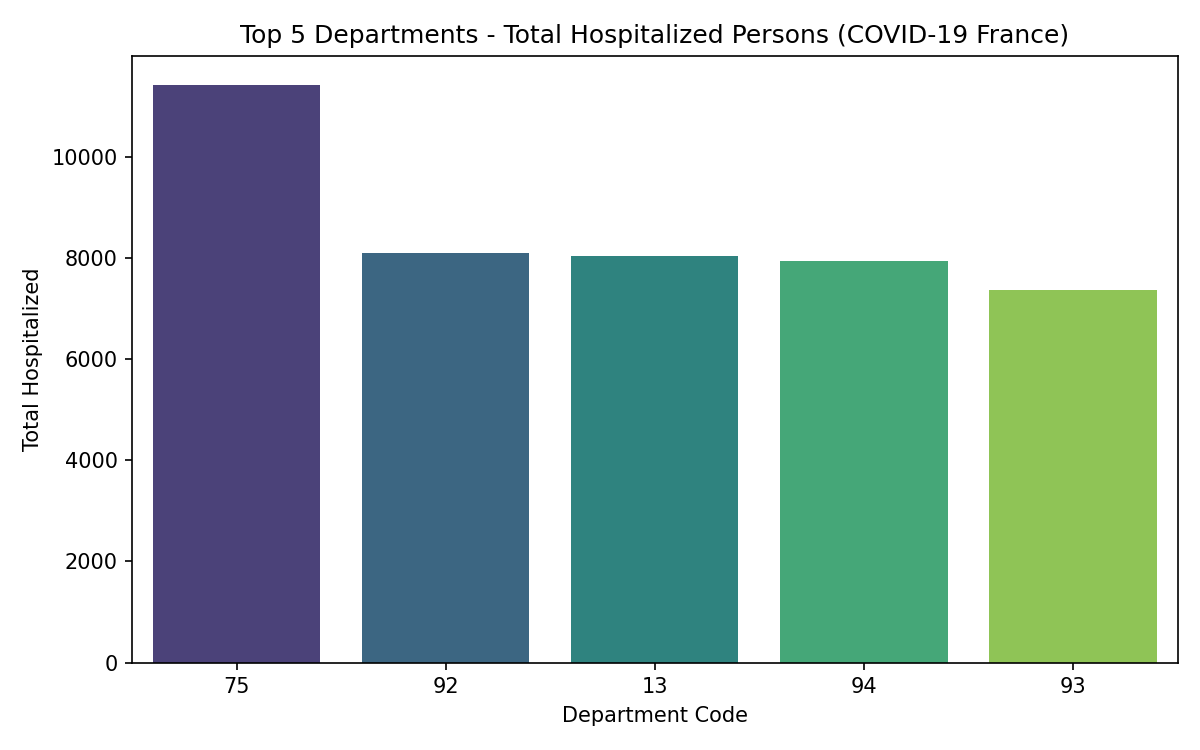
\includegraphics[width=0.85\textwidth]{practice set 01/deps.png}
\end{center}

% --- Q10 ---
\section*{Q10 — Filter Rhône Department / 筛选罗讷省 (69)}
\begin{lstlisting}
df_rhone = df[df['dep'] == 69]         # Department 69 = Rhône
print(f'Rhone data shape: {df_rhone.shape}')
\end{lstlisting}

% --- Q11 ---
\section*{Q11 — Deceased Trend in Rhône / 罗讷省死亡人数趋势}
\begin{lstlisting}
df_rhone = df_rhone.sort_values('date')
sns.lineplot(data=df_rhone, x='date', y='deceased',
             color='crimson', linewidth=1.5)
plt.title('Daily Deceased - Rhône (Department 69)')
plt.xlabel('Date')
plt.ylabel('Number of Deceased')
plt.xticks(rotation=45)
plt.show()
\end{lstlisting}

\begin{center}
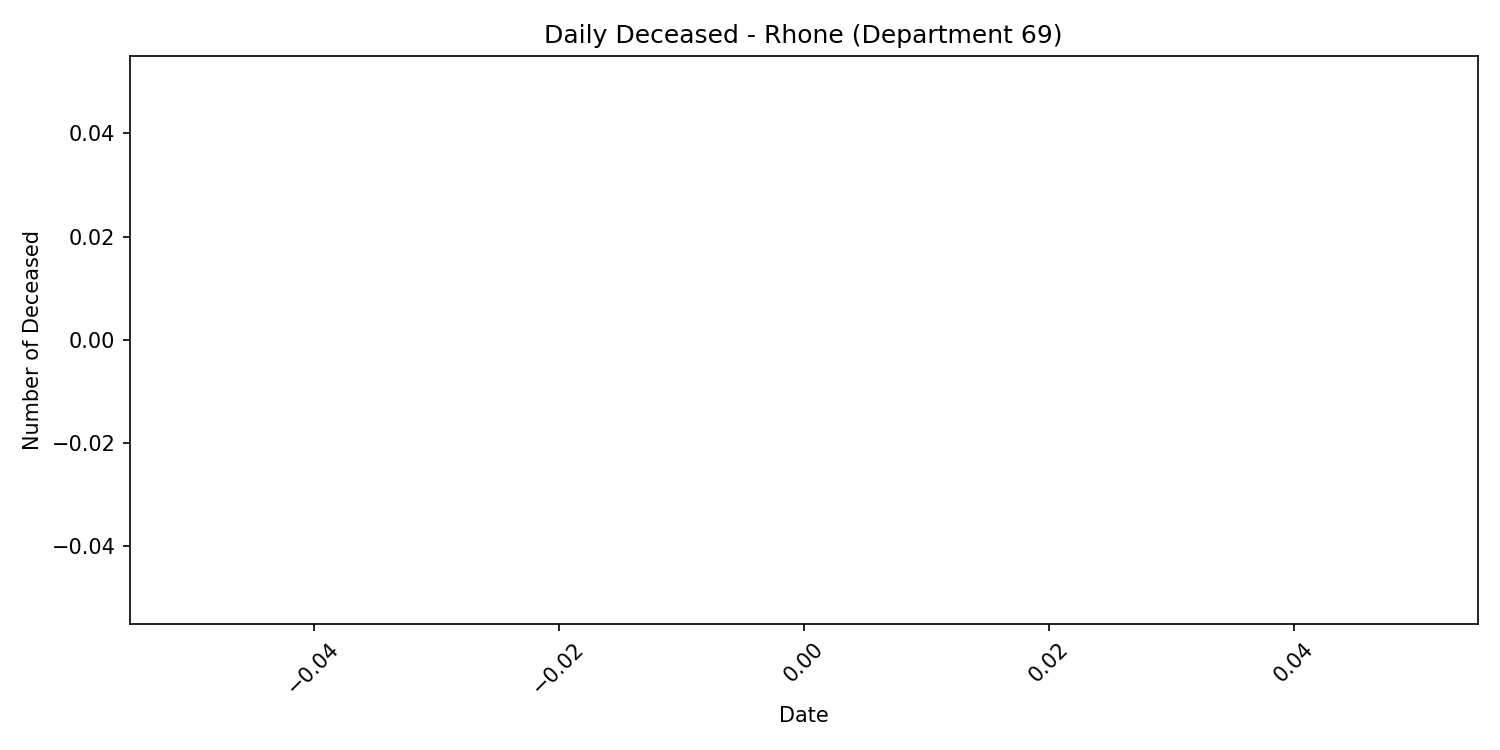
\includegraphics[width=0.95\textwidth]{practice set 01/rhones.png}
\end{center}

\begin{concept}{Key Takeaways / 核心收获}
    \begin{itemize}[itemsep=0.3em]
        \item \texttt{pd.read\_csv()} 读取 CSV → \texttt{.head()} / \texttt{.shape} 初探数据
        \item \texttt{.isnull().sum()} + \texttt{.dropna()} 处理缺失值
        \item \texttt{.rename(columns=\{...\})} 重命名列，使代码更可读
        \item \texttt{pd.to\_datetime()} 将字符串转为日期类型，解锁时间序列操作
        \item \texttt{.groupby('col').sum()} + \texttt{.reset\_index()} 分组聚合的标准套路
        \item \texttt{.sort\_values('col', ascending=False)} 降序排序
        \item \texttt{seaborn.barplot()} / \texttt{seaborn.lineplot()} 快速出图
    \end{itemize}
\end{concept}

\newpage

% ============================================================
\chapter{Practice Set 02 - Netflix Data Analysis / 练习题集 02 - Netflix 影视数据分析}
% ============================================================

\begin{concept}{Dataset Overview / 数据集概览}
    数据集 \texttt{netflix\_titles.csv} 来自 Flixable 提取的 Netflix 报告，共 8,804 条记录，包含电影和电视剧的元数据：
    \begin{itemize}[itemsep=0.2em]
        \item \textbf{type}：Movie or TV Show / 电影或电视剧
        \item \textbf{title}：Title of the content / 片名
        \item \textbf{director}：Director(s) name / 导演
        \item \textbf{cast}：List of actors (comma-separated) / 演员列表（逗号分隔）
        \item \textbf{country}：Production country(ies) / 制作国家
        \item \textbf{date\_added}：Date added to Netflix / 上线日期
        \item \textbf{release\_year}：Year of release / 发行年份
        \item \textbf{rating}：Content rating / 分级（如 PG-13, TV-MA）
        \item \textbf{duration}：Duration in min (Movie) or seasons (TV Show) / 时长
        \item \textbf{listed\_in}：Genre categories / 类型分类
        \item \textbf{description}：Summary text / 简介
    \end{itemize}
\end{concept}

\noindent\textbf{导入库 / Import Libraries：}
\begin{lstlisting}
import numpy as np
import pandas as pd
import matplotlib.pyplot as plt
import seaborn as sns
\end{lstlisting}

% --- Q1 ---
\section*{Q1 — Read File / 读取文件}
\begin{lstlisting}
nf = pd.read_csv('netflix_titles.csv')
print(nf.head(3))
print(f'Shape: {nf.shape}')        # (8804, 12)
\end{lstlisting}

% --- Q2 ---
\section*{Q2 — Data Summary / 数据摘要}
\begin{lstlisting}
print(nf.info())                    # Column types, non-null counts
print(nf.describe())                # Numerical summary
print(nf.describe(include='object')) # Categorical summary
\end{lstlisting}

% --- Q3 ---
\section*{Q3 — Unique Release Years / 唯一发行年份}
\begin{lstlisting}
unique_years = nf['release_year'].unique()
unique_years.sort()
print(unique_years)                 # e.g., [1925 1942 ... 2021]
print(f'Number of unique years: {len(unique_years)}')
\end{lstlisting}

% --- Q4 ---
\section*{Q4 — Time Period / 数据时间范围}
\begin{lstlisting}
print(f"From: {nf['release_year'].min()}")   # 1925
print(f"To:   {nf['release_year'].max()}")   # 2021
\end{lstlisting}

% --- Q5 ---
\section*{Q5 — Unique Movie Release Years / 仅电影的发行年份}
\begin{lstlisting}
movies = nf[nf['type'] == 'Movie']
movie_years = sorted(movies['release_year'].unique())
print(movie_years)
print(f'Movie years count: {len(movie_years)}')
\end{lstlisting}

% --- Q6 ---
\section*{Q6 — Average Movie Duration / 电影平均时长}
\begin{lstlisting}
# Duration column for movies: '90 min' → extract number
movies = nf[nf['type'] == 'Movie'].copy()
movies['duration_min'] = movies['duration'].str.extract(r'(\d+)').astype(float)
avg_duration = movies['duration_min'].mean()
print(f'Average movie duration: {avg_duration:.1f} minutes')
\end{lstlisting}

% --- Q7 ---
\section*{Q7 — Create Title → Cast Dictionary / 构建片名→演员字典}
\begin{lstlisting}
# Drop rows where cast is null / 删除演员为空的记录
nf_clean = nf.dropna(subset=['cast'])
titles_and_cast = dict(zip(nf_clean['title'], nf_clean['cast']))
print(f'Dictionary size: {len(titles_and_cast)} entries')
print(f'Example: {list(titles_and_cast.items())[0]}')
\end{lstlisting}

% --- Q8 ---
\section*{Q8 — Ryan Reynolds Appearances / Ryan Reynolds 出演次数}
\begin{lstlisting}
ryan_titles = [title for title, cast in titles_and_cast.items()
               if 'Ryan Reynolds' in cast]
print(f'Ryan Reynolds appears in {len(ryan_titles)} titles:')
for t in ryan_titles:
    print(f'  - {t}')
\end{lstlisting}

% --- Q9 ---
\section*{Q9 — Ryan Reynolds + Blake Lively Together / 夫妻档合作}
\begin{lstlisting}
together = [title for title, cast in titles_and_cast.items()
            if 'Ryan Reynolds' in cast and 'Blake Lively' in cast]
print(f'They appear together in {len(together)} titles:')
for t in together:
    print(f'  - {t}')
\end{lstlisting}

% --- Q10 ---
\section*{Q10 — Movies per Director / 各导演电影数量}
\begin{lstlisting}
# Filter to movies, drop null directors / 仅电影 + 排除空导演
movies_only = nf[nf['type'] == 'Movie'].copy()
movies_only = movies_only.dropna(subset=['director'])
director_counts = movies_only['director'].value_counts()
print(director_counts.head(15))
\end{lstlisting}

% --- Q11 ---
\section*{Q11 — Top 10 Directors / 前 10 名导演}
\begin{lstlisting}
top10_directors = director_counts.head(10)
print(top10_directors)
\end{lstlisting}

% --- Q12 ---
\section*{Q12 — Top 10 Directors Bar Chart / 前 10 名导演柱状图}
\begin{lstlisting}
sns.barplot(x=top10_directors.values, y=top10_directors.index,
            palette='magma')
plt.title('Top 10 Directors by Number of Movies (Netflix)')
plt.xlabel('Number of Movies')
plt.ylabel('Director')
plt.tight_layout()
plt.show()
\end{lstlisting}

\begin{center}
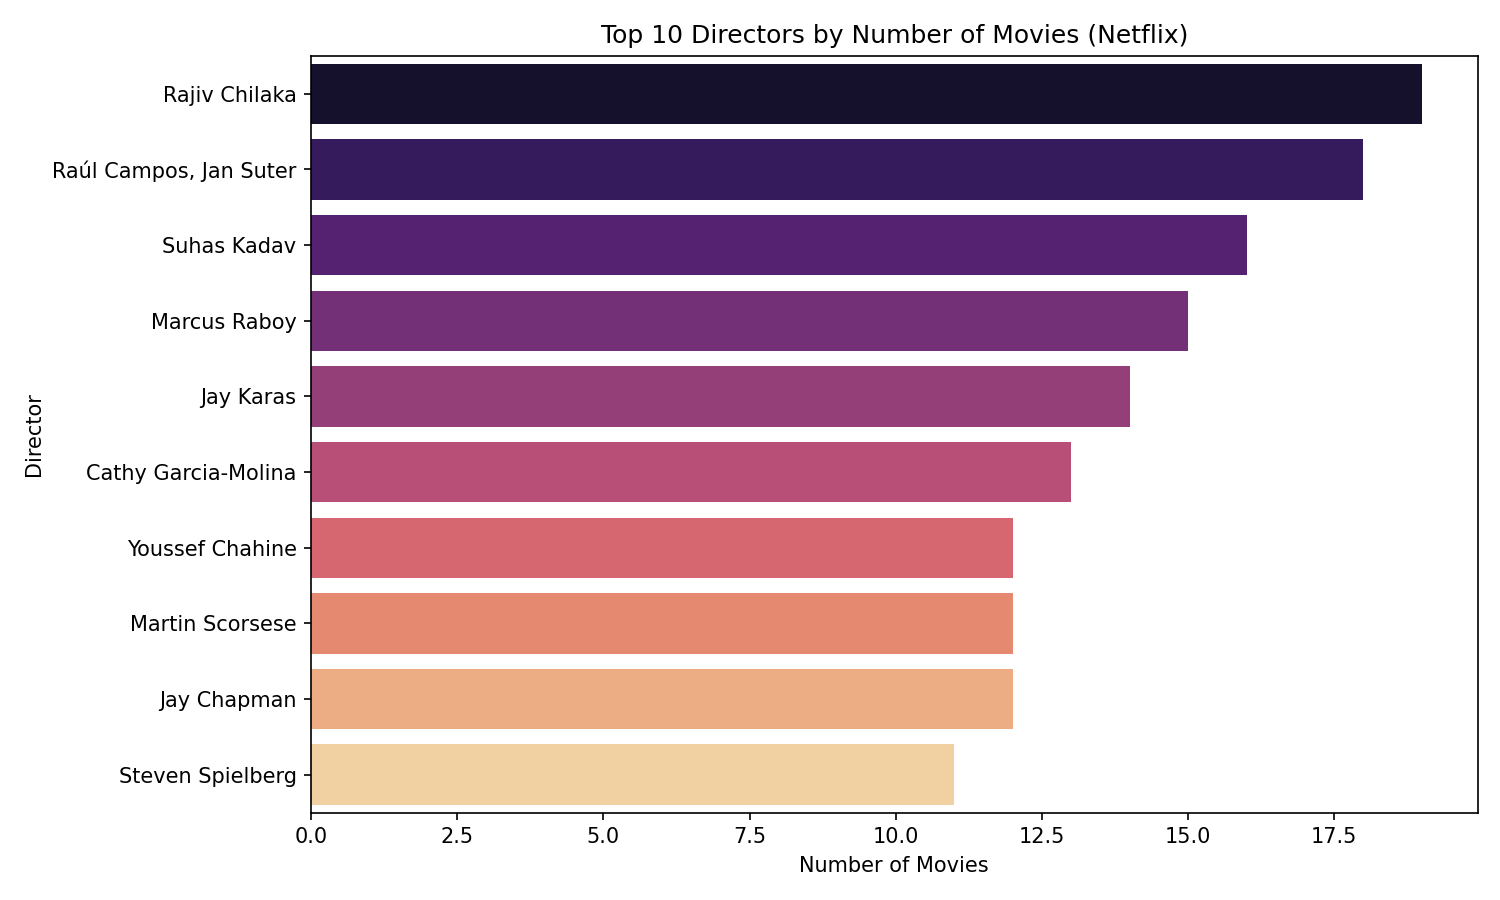
\includegraphics[width=0.95\textwidth]{practice set 02/directors.png}
\end{center}

\begin{concept}{Key Takeaways / 核心收获}
    \begin{itemize}[itemsep=0.3em]
        \item \texttt{.info()} + \texttt{.describe()} 是数据探索的第一步
        \item \texttt{.unique()} 提取唯一值 → \texttt{sorted()} 排序展示
        \item \texttt{.str.extract(r'(\textbackslash d+)')} 正则从字符串中提取数字
        \item \texttt{dict(zip(keys, values))} 两列快速转字典
        \item 字典推导式 + \texttt{if 'name' in cast} 做文本筛选，灵活高效
        \item \texttt{.value\_counts().head(10)} 是"Top-N 排行榜"的标准写法
        \item \texttt{seaborn.barplot()} 横向柱状图适合展示排名（\texttt{y=} 放类别标签）
    \end{itemize}
\end{concept}

\newpage

\appendix
\chapter{Complete Command Reference / 全课程命令速查表}

Below is a consolidated quick reference of all key syntax, functions, and methods covered in Chapters 01--09 plus Practice Sets. Use for exam review.
\vspace{1em}

% ====== 01 ======
\section*{01. Variables, Data Types \& Operators}
\small\renewcommand{\arraystretch}{1.3}
\centering
\begin{tabularx}{\textwidth}{@{}lX@{}}
\toprule
\textbf{Syntax} & \textbf{Description} \\ \midrule
\texttt{x = 10} & Assignment; value on RHS bound to name on LHS \\
\texttt{type(x)} & Return the data type of \texttt{x} \\
\texttt{print(x)} & Output \texttt{x} to console \\
\texttt{\# comment} & Single-line comment, ignored by Python \\
\texttt{None} & Null value (\texttt{NoneType}); not equal to 0, False, or \texttt{""} \\
\texttt{int(x) / float(x) / str(x) / bool(x)} & Type casting; \texttt{int(9.9) → 9} truncates (does not round) \\
\texttt{bool(0) → False} & Truthiness: 0, 0.0, \texttt{""}, \texttt{None}, \texttt{[]}, \texttt{\{\}} are falsy \\
\texttt{input(prompt)} & Read user input; \textbf{always returns str} \\
\texttt{// / ** / \%} & Floor division / exponent / modulo \\
\texttt{==  !=  <  >  <=  >=} & Comparison operators; result is always \texttt{bool} \\
\texttt{and / or / not} & Logical operators \\
\bottomrule
\end{tabularx}
\normalsize

% ====== Strings ======
\section*{Strings}
\small\renewcommand{\arraystretch}{1.3}
\centering
\begin{tabularx}{\textwidth}{@{}lX@{}}
\toprule
\textbf{Syntax} & \textbf{Description} \\ \midrule
\texttt{len(s)} & String length (includes spaces) \\
\texttt{s[i] / s[-i]} & Positive index (0-based) / Negative index (-1 = last char) \\
\texttt{s[start:stop]} & Slice; \textbf{inclusive:exclusive} (left-closed, right-open) \\
\texttt{s.lower() / s.upper()} & Convert to lower/upper case \\
\texttt{s.strip() / .lstrip() / .rstrip()} & Remove leading/trailing whitespace \\
\texttt{s.count(sub) / s.find(sub)} & Count occurrences / Find first index (-1 if not found) \\
\texttt{s.replace(old, new)} & Replace all occurrences; returns new string \\
\texttt{s.startswith(p) / s.endswith(p)} & Check prefix/suffix; returns \texttt{bool} \\
\texttt{s.split(d) / d.join(list)} & Split by delimiter / Join list with delimiter \\
\texttt{f"\{var\}"} & \textbf{f-string} (Python 3.6+); no \texttt{str()} needed \\
\texttt{"\{\} \{\}".format(a,b)} & \texttt{.format()} method \\
\texttt{"\%s" \% v} & Old-style \texttt{\%} formatting (legacy) \\
Escape chars: \texttt{\textbackslash n}, \texttt{\textbackslash t}, \texttt{\textbackslash\textbackslash}, \texttt{\textbackslash"} & Newline, tab, backslash, double-quote \\
\textbf{Immutability} & Strings are \textbf{immutable}; methods return new strings \\
\bottomrule
\end{tabularx}
\normalsize

% ====== 02 ======
\section*{02. Control Structures}
\small\renewcommand{\arraystretch}{1.3}
\centering
\begin{tabularx}{\textwidth}{@{}lX@{}}
\toprule
\textbf{Syntax} & \textbf{Description} \\ \midrule
\texttt{if cond: ... elif cond: ... else: ...} & Conditional branching \\
\texttt{for item in iterable: ...} & Iterate over each element in iterable \\
\texttt{for i in range(start, stop, step):} & Integer sequence loop; \textbf{inclusive:exclusive} \\
\texttt{while cond: ...} & Repeat while condition is True \\
\texttt{break} & Exit the innermost loop immediately \\
\texttt{continue} & Skip remaining code, jump to next iteration \\
\texttt{pass} & Placeholder; does nothing \\
\texttt{for i, val in enumerate(lst):} & Loop with both index and value \\
\texttt{for a, b in zip(l1, l2):} & Parallel iteration over multiple iterables \\
\texttt{[expr for x in lst if cond]} & \textbf{List comprehension} --- one-line list generation \\
\bottomrule
\end{tabularx}
\normalsize

% ====== 03 ======
\section*{03. Data Structures}
\small\renewcommand{\arraystretch}{1.3}
\centering
\begin{tabularx}{\textwidth}{@{}lX@{}}
\toprule
\textbf{Syntax} & \textbf{Description} \\ \midrule
\multicolumn{2}{@{}l@{}}{\textbf{List / 列表}} \\
\hspace{1em}\texttt{lst.append(x) / lst.extend(iter)} & Append element / Extend with all elements from iterable \\
\hspace{1em}\texttt{lst.insert(i, x) / lst.remove(x)} & Insert at index / Remove first match (error if missing) \\
\hspace{1em}\texttt{lst.pop(i) / lst.clear()} & Pop at index (default last) / Clear all elements \\
\hspace{1em}\texttt{lst.index(x) / lst.count(x)} & Find index of first match / Count occurrences \\
\hspace{1em}\texttt{lst.sort() / sorted(lst)} & In-place sort / Return new sorted list \\
\hspace{1em}\texttt{lst.reverse() / lst.copy()} & In-place reverse / Shallow copy \\
\hspace{1em}\texttt{del lst[i] / lst[i:j] = [...]} & Delete by index / Slice assignment \\
\midrule
\multicolumn{2}{@{}l@{}}{\textbf{Tuple / 元组 --- Immutable, hashable}} \\
\hspace{1em}\texttt{tup = (1, 2, 3) / tup = 1, 2, 3} & Create tuple (parentheses optional) \\
\hspace{1em}\texttt{a, b = tup} & Tuple unpacking \\
\midrule
\multicolumn{2}{@{}l@{}}{\textbf{Dictionary / 字典}} \\
\hspace{1em}\texttt{d = \{key: val\}} & Create dictionary \\
\hspace{1em}\texttt{d[key] / d.get(key, default)} & Access (error if key missing) / Safe access with fallback \\
\hspace{1em}\texttt{d.keys() / .values() / .items()} & Views of keys / values / key-value pairs \\
\hspace{1em}\texttt{d.update(\{k:v\}) / d.pop(key) / del d[key]} & Merge dict / Pop key / Delete key \\
\hspace{1em}\texttt{\{k:v for k,v in d.items() if cond\}} & Dict comprehension \\
\midrule
\multicolumn{2}{@{}l@{}}{\textbf{Set / 集合 --- Unordered, unique elements}} \\
\hspace{1em}\texttt{s = \{1,2,3\} / set(lst)} & Create set (auto-deduplicates) \\
\hspace{1em}\texttt{s.add(x) / s.remove(x) / s.discard(x)} & Add / Remove (error if missing) / Safe remove \\
\hspace{1em}\texttt{s | t / s \& t / s - t} & Union / Intersection / Difference \\
\bottomrule
\end{tabularx}
\normalsize

% ====== 04 ======
\section*{04. Functions \& Modules}
\small\renewcommand{\arraystretch}{1.3}
\centering
\begin{tabularx}{\textwidth}{@{}lX@{}}
\toprule
\textbf{Syntax} & \textbf{Description} \\ \midrule
\texttt{def f(a, b=default): ... return x} & Function definition with optional default argument \\
\texttt{lambda x, y: x + y} & Anonymous function; single expression only \\
\texttt{import numpy / import numpy as np} & Import entire module / Import with alias \\
\texttt{from math import sqrt, pi} & Import specific names from module \\
\texttt{from module import *} & Import all public names (discouraged) \\
\texttt{dir(obj) / help(func)} & List attributes and methods / View docstring \\
\texttt{if \_\_name\_\_ == "\_\_main\_\_":} & Script entry-point guard: runs only when executed directly \\
\texttt{pip install package} & Install third-party package via terminal \\
\bottomrule
\end{tabularx}
\normalsize

% ====== 05 ======
\section*{05. Object-Oriented Programming}
\small\renewcommand{\arraystretch}{1.3}
\centering
\begin{tabularx}{\textwidth}{@{}lX@{}}
\toprule
\textbf{Syntax} & \textbf{Description} \\ \midrule
\texttt{class Dog:} & Class definition \\
\texttt{def \_\_init\_\_(self, name):} & Constructor; \texttt{self} refers to the instance \\
\texttt{self.name = name} & Instance attribute; unique to each object \\
\texttt{d = Dog("Buddy")} & Instantiation (automatically calls \texttt{\_\_init\_\_}) \\
\texttt{class Puppy(Dog):} & Inheritance: Puppy inherits all attributes/methods from Dog \\
\texttt{super().\_\_init\_\_(...)} & Call parent constructor from child class \\
\texttt{super().method()} & Call any parent method \\
\texttt{@property} & Decorator: turn method into attribute-like access (getter) \\
\texttt{@staticmethod} & Static method; no \texttt{self} parameter needed \\
\texttt{@classmethod} & Class method; first parameter is \texttt{cls}, not \texttt{self} \\
\texttt{\_\_str\_\_(self)} & String representation; called by \texttt{print(obj)} and \texttt{str(obj)} \\
\texttt{\_\_repr\_\_(self)} & Developer representation; called by \texttt{repr(obj)} \\
\bottomrule
\end{tabularx}
\normalsize

% ====== 06 ======
\section*{06. File I/O \& Error Handling}
\small\renewcommand{\arraystretch}{1.3}
\centering
\begin{tabularx}{\textwidth}{@{}lX@{}}
\toprule
\textbf{Syntax} & \textbf{Description} \\ \midrule
\texttt{open('f.txt', 'r')} & Read mode; file must exist \\
\texttt{open('f.txt', 'w')} & Write mode; \textbf{overwrites existing content}! \\
\texttt{open('f.txt', 'a')} & Append mode; adds content at end of file \\
\texttt{with open('f.txt') as f:} & \textbf{Recommended}: context manager auto-closes file \\
\texttt{f.write(str)} & Write string to file; \textbf{does NOT add newline automatically} \\
\texttt{f.read()} & Read entire file as a single string \\
\texttt{f.readline()} & Read one line (includes trailing newline) \\
\texttt{f.readlines()} & Read all lines into a list of strings \\
\texttt{for line in f:} & Iterate line by line; \textbf{most memory-efficient} \\
\texttt{f.close()} & Manually close file (unnecessary with \texttt{with}) \\
\texttt{csv.reader(f) / csv.DictReader(f)} & CSV reader returning lists / dicts (\textbf{DictReader recommended}) \\
\texttt{csv.writer(f).writerow(row)} & Write one row to CSV file \\
\texttt{try: ... except ErrType: ... else: ... finally:} & Full exception handling structure \\
\texttt{SyntaxError / IndentationError} & Invalid Python syntax / Wrong indentation \\
\texttt{NameError / TypeError / ValueError} & Undefined variable / Wrong type operation / Invalid value \\
\texttt{IndexError / KeyError} & List index out of range / Dictionary key not found \\
\texttt{AttributeError / FileNotFoundError} & Missing attribute/method / File does not exist \\
\texttt{ZeroDivisionError} & Division by zero \\
\bottomrule
\end{tabularx}
\normalsize

% ====== PEP-8 ======
\section*{PEP-8 Quick Reference}
\small\renewcommand{\arraystretch}{1.3}
\centering
\begin{tabularx}{\textwidth}{@{}lX@{}}
\toprule
\textbf{Rule} & \textbf{Convention} \\ \midrule
Variables and functions & \texttt{snake\_case}: lowercase with underscores \\
Constants & \texttt{UPPER\_CASE\_WITH\_UNDERSCORES} \\
Classes & \texttt{UpperCamelCase} (PascalCase) \\
Blank lines & 2 blank lines between functions; 1 between code blocks \\
Operators & Spaces around operators: \texttt{x = a + b} \\
Commas & Space after comma: \texttt{f(a, b, c)} \\
Keyword arguments & No space around \texttt{=}: \texttt{f(n=42)} \\
Function call & No space before \texttt{(}: \texttt{func(x)} \\
Line length & Max 79 characters; break long lines with \texttt{\textbackslash} or parentheses \\
Naming conflicts & Never use \texttt{list}, \texttt{str}, \texttt{int}, \texttt{print} as variable names \\
\bottomrule
\end{tabularx}
\normalsize

% ====== 07 ======
\section*{07. Matplotlib Visualization}
\small\renewcommand{\arraystretch}{1.3}
\centering
\begin{tabularx}{\textwidth}{@{}lX@{}}
\toprule
\textbf{Syntax} & \textbf{Description} \\ \midrule
\texttt{\%matplotlib inline} & Enable inline display in Jupyter Notebook \\
\texttt{import matplotlib.pyplot as plt} & Import matplotlib's pyplot interface \\
\texttt{fig, ax = plt.subplots()} & Create figure and axes objects (\textbf{recommended style}) \\
\texttt{fig, axes = plt.subplots(nrows, ncols)} & Create a grid of subplots \\
\texttt{ax.plot(x, y)} & Line plot \\
\texttt{ax.scatter(x, y)} & Scatter plot \\
\texttt{ax.bar(x, height)} & Vertical bar chart \\
\texttt{ax.hist(data, bins)} & Histogram \\
\texttt{ax.boxplot(data)} & Box plot \\
\texttt{ax.set\_title('title')} & Set chart title \\
\texttt{ax.set\_xlabel('label') / set\_ylabel('label')} & Set axis labels \\
\texttt{ax.set\_xlim(lo, hi) / set\_ylim(lo, hi)} & Set axis range limits \\
\texttt{ax.legend(loc=, frameon=)} & Display legend; \texttt{loc='best'} for automatic placement \\
\texttt{ax.grid(True)} & Add background grid \\
\texttt{ax.axis('off')} & Hide all axis elements \\
\texttt{plt.tight\_layout()} & Auto-adjust spacing between subplots \\
\texttt{plt.savefig('f.png', dpi=300)} & Save current figure to file \\
\texttt{plt.show()} & Display the figure \\
Color specification & \texttt{'r','b','g','k','w'} letters / hex \texttt{\#0000FF} / RGB \texttt{(0,0,1,0.5)} / grayscale \texttt{'0.5'} / cycle \texttt{'C0'--'C9'} \\
Markers & \texttt{'o'} circle, \texttt{'s'} square, \texttt{'D'} diamond, \texttt{'\^'} triangle, \texttt{'*'} star \\
Linestyles & \texttt{'-'} solid, \texttt{'--'} dashed, \texttt{':'} dotted, \texttt{'-.′} dash-dot \\
\bottomrule
\end{tabularx}
\normalsize

% ====== 08 ======
\section*{08. Pandas I --- Data Manipulation}
\small\renewcommand{\arraystretch}{1.3}
\centering
\begin{tabularx}{\textwidth}{@{}lX@{}}
\toprule
\textbf{Syntax} & \textbf{Description} \\ \midrule
\texttt{import pandas as pd} & Import Pandas library \\
\texttt{pd.read\_csv('f.csv')} & Read CSV file into DataFrame \\
\texttt{pd.read\_excel('f.xlsx')} & Read Excel file into DataFrame \\
\texttt{pd.DataFrame(dict)} & Create DataFrame from dictionary \\
\texttt{df.head(n) / df.tail(n)} & View first/last n rows (default: 5) \\
\texttt{df.shape} & Return (rows, columns) tuple \\
\texttt{df.columns / df.index} & Column names / Row index \\
\texttt{df.dtypes / df.info()} & Data types of each column / DataFrame info summary \\
\texttt{df.describe()} & Statistics: count, mean, std, min, 25\%, 50\%, 75\%, max \\
\texttt{df.isna().sum()} & Count missing values per column; \texttt{isnull()} is equivalent \\
\texttt{df.dropna(inplace=True)} & Drop rows containing any NaN \\
\texttt{df.fillna(value)} & Replace all NaN values with \texttt{value} \\
\texttt{df.drop(columns=['c'])} & Drop specified columns \\
\texttt{df.rename(columns=\{old:new\})} & Rename columns \\
\texttt{df.astype('category')} & Convert column type (saves memory for low-cardinality data) \\
\texttt{df.sort\_values('c', ascending=False)} & Sort by column; can pass list for multi-column sort \\
\texttt{df['c'].unique()} & Return array of unique values \\
\texttt{df['c'].value\_counts()} & Return frequency of each unique value \\
\texttt{df.loc[cond, cols]} & \textbf{Label-based indexing}: select by row label and column name \\
\texttt{df.iloc[i, j]} & \textbf{Integer-based indexing}: select by row/column position \\
\texttt{df.at[label, 'col'] / df.iat[i, j]} & Fast access to single scalar value \\
\texttt{df[df['col'] > 100]} & Boolean filtering: select rows meeting condition \\
\bottomrule
\end{tabularx}
\normalsize

% ====== 09 ======
\section*{09. Pandas II --- Feature Engineering \& Aggregation}
\small\renewcommand{\arraystretch}{1.3}
\centering
\begin{tabularx}{\textwidth}{@{}lX@{}}
\toprule
\textbf{Syntax} & \textbf{Description} \\ \midrule
\texttt{df.assign(new=lambda x: expr)} & Create new column using lambda expression \\
\texttt{df.groupby('col').mean()} & Group by column, compute mean (also sum, min, max, count, std) \\
\texttt{df.groupby('col').agg(['mean','std'])} & Apply multiple aggregation functions at once \\
\texttt{df.groupby(['c1','c2']).size()} & Group by multiple columns, count group sizes \\
\texttt{df.pivot\_table(index, columns, values, aggfunc)} & \textbf{Pivot table}: multi-dimensional aggregation \\
\texttt{pd.crosstab(index, columns)} & \textbf{Crosstab}: frequency table of two categorical variables \\
\texttt{pd.cut(data, bins, labels)} & \textbf{Binning}: discretize continuous values into categories \\
\texttt{pd.qcut(data, q)} & Quantile-based binning \\
\texttt{pd.get\_dummies(df, columns=['c'])} & \textbf{One-hot encoding}: create binary indicator columns \\
\texttt{LabelEncoder().fit\_transform(series)} & \textbf{Label encoding}: convert strings to integers (sklearn) \\
\texttt{pd.merge(a, b, on='key', how='left')} & SQL-style merge; how = left/right/inner/outer \\
\texttt{pd.concat([df1, df2], axis=0)} & Concatenate DataFrames along rows (axis=0) or columns (axis=1) \\
\texttt{df.plot(kind='bar', rot, figsize, title)} & Pandas integrated plotting (calls Matplotlib internally) \\
\texttt{pd.set\_option('display.max\_columns', n)} & Configure Pandas display options \\
\bottomrule
\end{tabularx}
\normalsize

\end{document}
